\documentclass[11pt]{article}
\usepackage[a4paper,margin=1in]{geometry}
\usepackage{amsmath,amssymb,amsthm,mathtools,graphicx,booktabs,microtype}
\usepackage[authoryear,round]{natbib}
\usepackage{longtable,array,enumitem,float,needspace,placeins}
\usepackage[hidelinks]{hyperref}
\emergencystretch=1em
\setcounter{topnumber}{5}\setcounter{bottomnumber}{4}\setcounter{totalnumber}{8}
\renewcommand{\topfraction}{0.95}\renewcommand{\bottomfraction}{0.95}
\renewcommand{\textfraction}{0.05}\renewcommand{\floatpagefraction}{0.75}
\setlist{nosep,leftmargin=1.5em}
\newtheorem{theorem}{Theorem}[section]
\newtheorem{proposition}[theorem]{Proposition}
\newtheorem{corollary}[theorem]{Corollary}
\newtheorem{lemma}[theorem]{Lemma}
\theoremstyle{definition}\newtheorem{definition}[theorem]{Definition}
\theoremstyle{remark}\newtheorem{remark}[theorem]{Remark}
\newcommand{\E}{\mathbb E}\newcommand{\Prob}{\mathbb P}\newcommand{\R}{\mathbb R}
\newcommand{\KL}{D_{\mathrm{KL}}}\newcommand{\ES}{\operatorname{ES}}\newcommand{\VaR}{\operatorname{VaR}}
\newcommand{\Wone}{W_1}\newcommand{\ind}{\mathbf 1}\newcommand{\softplus}{\operatorname{softplus}}
\newcommand{\inputrows}[1]{\input{#1}}
\title{Parametric and Nonparametric Models of Joint Returns: Density, Dependence, and Portfolio Tail Risk}
\author{Miquel Noguer i Alonso\\Artificial Intelligence Finance Institute}
\date{November 7, 2026\\[0.4em]\small DOI: \href{https://doi.org/10.5281/zenodo.24024955}{10.5281/zenodo.24024955}}
\begin{document}
\maketitle
\begin{abstract}
We compare parametric, empirical and neural models of joint asset returns to determine whether greater flexibility improves density, dependence and portfolio risk. Gaussian, shrinkage-Gaussian, Student and meta-$t$ laws provide parametric benchmarks; meta-$t$ joins asset-specific Student margins with a Student copula. Filtered historical simulation (FHS) supplies empirical innovations. Normalizing flows learn invertible density transformations, variational autoencoders learn latent-variable distributions, and Wasserstein GANs learn scenario generators. Separate volatility and correlation controls distinguish conditioning from innovation modeling. Ten estimation datasets per Student, meta-$t$ and Heston synthetic law, and 2,514 CRSP test dates in five-basket and 100-stock panels, support paired comparisons with multiplicity control. Meta-$t$ achieves the best observed exact density fit in both CRSP panels. Under common one-percent validation selection, no tested neural model establishes a risk-score improvement over FHS; alternative checkpoint rules change rankings. Student's 100-stock advantage depends on the comparison family. Variance filtering produces the largest point-score gains, with inconclusive adjusted tests. Synthetic results distinguish correct specification from architectural flexibility and separate likelihood quality from expected-shortfall accuracy. A Wishart--CIR extension relaxes a restricted covariance model's dispersion ceiling but fails the conditional numerical-stability gate. The evidence makes conditioning, specification and validation design central to assessing distributional flexibility.

\end{abstract}

\section{Introduction}
A multivariate return model must describe each asset's risk and how assets move together, then translate that joint law into portfolio outcomes. We ask when a structured parametric distribution is sufficient and when empirical or neural flexibility improves this task. The comparison separates three objectives: fitting the joint density, reproducing downside dependence, and forecasting portfolio Value-at-Risk (VaR) and expected shortfall (ES). Density measures the whole distribution, dependence measures joint downside events, and risk forecasts measure losses on fixed portfolio exposures. These objectives can favor different fitted models.

\paragraph{What is compared.}
Gaussian, shrinkage-Gaussian, multivariate Student and meta-$t$ laws provide structured joint distributions. FHS combines empirical innovations with a volatility filter. Normalizing flows learn invertible distributional transformations, VAEs use latent-variable decoders, and Wasserstein GANs learn scenario samplers \citep{papamakarios2021review,kingma2014vae,goodfellow2014gan}. A fixed neural network is itself finitely parameterized; ``neural'' and ``nonparametric'' are therefore distinct classifications. We also examine coordinate- and portfolio-GARCH controls, five-basket dynamic conditional correlation (DCC), a restricted Heston--Wishart stochastic-covariance specification, and an additive Wishart--CIR extension.

The neural comparison concerns static innovation laws fitted annually, and static five-day joint windows in the Heston experiment. Conditional forecasts arise from separately specified filters; the networks do not learn a recursive state-conditioned generator. The bounded flow architectures, their dense-output controls, and training budgets are stated explicitly. The results therefore describe these implementations rather than all possible neural models or conditional time-series generators such as Quant GAN \citep{wiese2020quantgan,buehler2020simulator}.

\paragraph{Main findings.}
Table~\ref{tab:r5-summary} collects the evidence that organizes the paper. Variance conditioning accounts for the largest observed CRSP score gains, although the adjusted tests do not resolve those effects. Within the common primary filter, the Student gain in 100 stocks is sensitive to the comparison family, and no tested neural innovation model establishes an adjusted improvement over FHS. In controlled Heston data, analytic Student ES exposes a clear density--risk discrepancy. Theoretical tail classes explain representation restrictions; finite-level experiments determine whether the tested restrictions have detectable practical consequences.
\begin{table}[htbp]
\centering\footnotesize
\setlength{\tabcolsep}{4pt}
\begin{tabular}{lll}
\toprule
Comparison & Observed result & Scope / reference \\
\midrule
Variance conditioning & $-0.055$ / $-0.115$ & Five / 100; Holm/6 $p=0.072/0.096$ \\
Incremental EVT & $-0.005$ / $+0.002$ & Score unresolved; CM: see caption \\
Student versus FHS & $-0.023$ & 100 stocks; Holm $0.0352$ / $0.0594$ \\
Heston Student fit & NLL 28.480; RMSE 2.841 & Gaussian: 31.500; 1.508 \\
Heston level transfer & Flow-t: 0.243 / 1.635 & ES RMSE at 1\% / 0.1\% \\
\bottomrule
\end{tabular}
\caption{Five comparisons that organize the study. FZ0 differences are negative when the named change improves the point score. Variance-conditioning magnitudes depend on the missing-return convention (Table~\ref{tab:missing100}). The unadjusted conditional-moment (CM) diagnostic rejects GARCH-FHS in both panels ($p<0.001$) but not GARCH-EVT ($p=0.271/0.394$; Table~\ref{tab:r4-calibration}). Student p-values refer to the primary and broader retrospective families. RMSE and NLL are distinct objectives; no row asserts universal model dominance.}\label{tab:r5-summary}
\end{table}


Our contributions are:
\begin{enumerate}
\item An integrated experimental design that separates joint-law specification, predictable filtering, and checkpoint selection through matched data, paired uncertainty and explicit multiplicity families.
\item A one-sided loss-tail result distinguishing elliptical from independent Student latent noise, together with a residual meta-$t$ flow whose marginal indices are controlled.
\item Evidence on where these distinctions matter: favorable parametric specification in synthetic laws, the Heston density--risk discrepancy, selection-sensitive neural rankings, and the separate roles of volatility and dependence.
\item A stochastic-covariance specification study: an admissibility-induced dispersion ceiling, an additive scalar-variance repair, and a frozen-law equivalence showing why static fit alone cannot identify the value of stochastic correlation.
\end{enumerate}
The controlled laws isolate specification and representation; the chronological CRSP panels evaluate conditional forecasting. Matched filter controls attribute changes in point scores, checkpoint alternatives assess selection sensitivity, and paired inference quantifies the resolution of each comparison. Longer derivations, secondary comparisons and numerical audits are in the appendices.

\paragraph{Relation to existing work.}
The meta-elliptical construction and $t$ copula, including heterogeneous Student margins, are the established Fang--Fang--Kotz and Demarta--McNeil object \citep{fang2002meta,demarta2005tcopula}. We use that established distribution; the application and residual-flow construction are the contributions here. Its portfolio application is discussed by \citet{noguer2025metat}. Tail restrictions of Lipschitz flows and adaptive bases are developed by \citet{jaini2020tails,laszkiewicz2022tail}. EV-GAN studies extreme-value parametrizations of ReLU generators \citep{allouche2022evgan}; our noise-law distinction should be read alongside that literature, not as a claim that neural heavy-tail analysis begins here. Tail-GAN directly uses joint VaR--ES elicitability to train risk-sensitive scenario generators \citep{cont2025tailgan}, motivating a common decision-relevant checkpoint criterion. Our validation criterion does not turn the implemented WGAN into Tail-GAN, whose training objective is different. COMET combines copula modeling and extreme-value margins \citep{mcdonald2022comet}; it is closely related in purpose to marginal tail control with flexible dependence.

Expected-shortfall representations, the Wasserstein risk bound, and the forward-KL obstruction are background tools, not new general risk theory \citep{acerbi2002coherence,rockafellar2002cvar,esfahani2018}. Joint VaR--ES scoring follows \citet{fissler2016,patton2019}; conditional-moment backtesting follows \citet{nolde2017}. We use the model confidence set of \citet{hansen2011mcs} for the question of which forecasts can be distinguished from the best. Standard Heston mixture and transform calculations appear in Appendix~\ref{sec:heston}. EVT supplies both the radial-splice diagnostic and the additional conditional tail benchmark \citep{pickands1975,balkema1974,breiman1965,mcneil2000evt}.

\section{Probability, tail classes, and the three objectives}\label{sec:objectives}
For $X\in\R^d$, write $\|X\|$ for its Euclidean norm. For a fixed portfolio vector $w$, the idealized linear loss is $L=-w^\top X$. With $\alpha\in(0,1)$ denoting a tail probability,
\begin{equation}\label{eq:es}
\VaR_\alpha(L)=F_L^{-1}(1-\alpha),\qquad
\ES_\alpha(L)=\alpha^{-1}\int_{1-\alpha}^1F_L^{-1}(u)\,du.
\end{equation}
For an integrable loss, ES also has the dual representation
\begin{equation}\label{eq:dual}
\ES_\alpha(L)=\sup\{\E[\zeta L]:0\le\zeta\le\alpha^{-1},\ \E\zeta=1\}.
\end{equation}
We distinguish a \emph{logarithmic radial index},
$\log\Prob(\|X\|>r)/\log r\to-\nu$, from \emph{regular variation},
$\Prob(\|X\|>r)=r^{-\nu}\ell(r)$ with $\ell$ slowly varying. The former alone neither supplies an exact tail constant nor implies the latter. The CRSP application uses arithmetic returns: a long-only one-day loss is bounded by 100\%, whereas the architectural tail statements concern idealized unbounded laws. The empirical task evaluates finite probability levels, not an infinite-loss tail index. A Gaussian-order tail means $-\log\Prob(\|X\|>r)=\Theta(r^2)$; exponential-order means $\Theta(r)$. A sub-Gaussian upper bound does not assert a matching lower bound.

\subsection{Normalizing flows}
For a differentiable bijection $T_\theta$ with nonsingular Jacobian and a positive base density $p_Z$,
\begin{equation}\label{eq:flow-density}
q_\theta(x)=p_Z(T_\theta^{-1}(x))|\det DT_\theta^{-1}(x)|.
\end{equation}
When the integrals exist, $\E_p[-\log q_\theta(X)]=H(p)+\KL(p\|q_\theta)$. Exact likelihood therefore identifies the population objective, not a finite-sample guarantee for a tail functional. Affine coupling layers use
\begin{equation}\label{eq:coupling}
x_c=z_c,\qquad x_d=z_d\odot\exp(s(z_c))+t(z_c),
\end{equation}
with log Jacobian $\sum_i s_i(z_c)$ \citep{dinh2017realnvp}.

\subsection{Variational autoencoders}
A VAE specifies $Z\sim\pi$, $X\mid Z\sim p_\theta(\cdot\mid Z)$, and an encoder $q_\phi(z\mid x)$. The identity
\begin{equation}\label{eq:elbo}
\log p_\theta(x)=\E_{q_\phi}\log p_\theta(x\mid Z)-\KL(q_\phi(\cdot\mid x)\|\pi)
+\KL(q_\phi(\cdot\mid x)\|p_\theta(\cdot\mid x))
\end{equation}
separates marginal likelihood from the variational gap. The Gaussian decoder is $X=\mu(Z)+\operatorname{diag}(\sigma(Z))C_\varepsilon\varepsilon$, with independent $\varepsilon\sim N(0,I)$ and a fixed nonsingular $C_\varepsilon$. The expectation of the IWAE-$K$ log importance-weight average is a lower bound on log likelihood \citep{burda2016iwae}. A realized Monte Carlo IWAE estimate is not a deterministic bound. Therefore its negative is upward-biased in expectation conditional on the observations and fitted model. If a VAE has a lower estimated NLL than an exact-density competitor, the variational bias works against the VAE: that ordering is conservative with respect to the expected importance-sampling gap. A single realized estimate still has Monte Carlo noise, so it does not certify an ordering. Tables identify this distinction explicitly.

\subsection{GANs and Wasserstein critics}
For the original GAN objective, maximizing over an unrestricted discriminator gives $-\log4+2\operatorname{JS}(p,q_\theta)$ \citep{goodfellow2014gan}. WGAN instead uses the dual formulation
\begin{equation}\label{eq:wgan}
\Wone(p,q)=\sup_{\|f\|_{\rm Lip}\le1}\{\E_pf-\E_qf\}.
\end{equation}
A restricted globally 1-Lipschitz critic provides a lower bound on this supremum. A gradient penalty at sampled interpolants is a training regularizer, not a global Lipschitz certificate \citep{arjovsky2017wgan,gulrajani2017wgangp}. Neither its reported objective nor a neural lower bound is an upper certificate for ES error.

\paragraph{Why separate the objectives?}
For integrable loss laws, $|\ES_\alpha(P)-\ES_\alpha(Q)|\le W_1(P,Q)/\alpha$, while a small forward KL divergence alone gives no unrestricted ES-error bound. Theorem~\ref{thm:w1} and Proposition~\ref{prop:kl} state these standard facts precisely. They motivate measuring density and risk separately; they do not predict a finite-sample ranking.
\section{Architectural tail restrictions}\label{sec:architecture}
\subsection{Flows: radial versus coordinatewise control}
\begin{theorem}[Linear-growth tail bounds]\label{thm:growth}
Let $X=T(Z)$, with constants $C>0$ and $B\ge0$. If $\|T(z)\|\le C\|z\|+B$, then for $r>B$,
$\Prob(\|X\|>r)\le\Prob(\|Z\|>(r-B)/C)$.
If also $\|T(z)\|\ge c\|z\|-b$ for $c>0$ and $b\ge0$, then
\begin{equation}\label{eq:sandwich}
\Prob(\|Z\|>(r+b)/c)\le\Prob(\|X\|>r)
\le\Prob(\|Z\|>(r-B)/C).
\end{equation}
Under these two bounds, $Z$ has a finite logarithmic radial tail index $\nu$ if and only if $X$ does, with the same index. For each $k>0$, their $k$th norm moments are finite simultaneously. For a standard Gaussian $Z$, the output has Gaussian-order radial tails.
\end{theorem}
\noindent\emph{Proof.} See Appendix~\ref{app:proofs}.

\begin{corollary}[Bounded affine coupling]\label{cor:coupling}
If each layer \eqref{eq:coupling} satisfies $|s_i|\le\bar s$ and $|t_i|\le\bar t$, then it satisfies Theorem~\ref{thm:growth} with $c=e^{-\bar s}$, $C=e^{\bar s}$, and $b=B=\sqrt d\bar t$. A finite composition and any invertible affine output map retain two-sided linear norm growth.
\end{corollary}
\noindent\emph{Proof.} See Appendix~\ref{app:proofs}.

\begin{proposition}[Marginal indices require marginal bounds]\label{prop:marginal}
For a finite composition of bounded-scale, bounded-shift coupling layers, coordinate permutations, and nonsingular diagonal affine maps, there is a permutation $\pi$ and constants $c_i,C_i>0$, $b_i,B_i\ge0$ such that
\begin{equation}\label{eq:coordinate}
c_i|Z_{\pi(i)}|-b_i\le |X_i|\le C_i|Z_{\pi(i)}|+B_i.
\end{equation}
Thus each finite logarithmic marginal tail index is preserved, up to permutation. A norm bound alone does not imply this statement, and an arbitrary dense affine mixing layer does not generally preserve heterogeneous marginal indices.
\end{proposition}
\noindent\emph{Proof.} See Appendix~\ref{app:proofs}.

These propositions concern a fixed transformation. They do not imply that a tail parameter in the base law cannot be trained. Nor do they imply that unbounded log scales are the only way to change a tail. The triangular map $(z_1,z_2)\mapsto(z_1,z_2+z_1^3)$ is invertible, has determinant one, and changes the second marginal tail through an unbounded shift. Logarithmic index preservation should not be strengthened silently to regular variation: bounded oscillating scale factors can obstruct a limiting tail ratio.

\subsection{Gaussian decoders}
\begin{proposition}[Bounded decoders]\label{prop:bounded-vae}
Let $X_i=\mu_i(Z)+\sigma_i(Z)\eta_i$, where $\eta_i\sim N(0,s_i^2)$ is independent of $Z$, $|\mu_i|\le M$, and $0\le\sigma_i\le\bar\sigma$. Then for $r>M$,
\begin{equation}
\Prob(|X_i|>r)\le2\exp\{-(r-M)^2/(2s_i^2\bar\sigma^2)\}.
\end{equation}
This upper bound holds for every prior on $Z$. If $s_i>0$ and $\Prob(\sigma_i(Z)\ge a)>0$ for some $a>0$, the tail is Gaussian-order. A union bound gives a corresponding norm bound in finite dimension.
\end{proposition}
\noindent\emph{Proof.} See Appendix~\ref{app:proofs}.

\begin{theorem}[Growth of a Gaussian decoder scale]\label{thm:scale}
Let $Z\sim N(0,I_{m_z})$ and $\eta\sim N(0,s^2)$ be independent, with $s>0$, and $X=\mu(Z)+\sigma(Z)\eta$, $|\mu|\le M$. For $\beta>0$ and constants $C,c>0$, assume $0\le\sigma(z)\le C(1+\|z\|^\beta)$ everywhere and $\sigma(z)\ge c\|z\|^\beta$ for sufficiently large $\|z\|$ on a cone with positive spherical measure. Then
\begin{equation}\label{eq:scale-exponent}
-\log\Prob(|X|>r)=\Theta(r^{2/(\beta+1)}).
\end{equation}
In particular, linear growth on a cone gives exponential-order tails. If instead $\sigma(z)\le\exp(C\|z\|+D)$ everywhere and $\sigma(z)\ge\exp(c\|z\|-D)$ on such a cone for large radius, then $-\log\Prob(|X|>r)=\Theta((\log r)^2)$.
\end{theorem}
\noindent\emph{Proof.} See Appendix~\ref{app:proofs}.

A head $\softplus(a^\top z+g(z))$, with $a\ne0$ and bounded $g$, has a linear lower bound on a positive cone; it does not have a lower bound proportional to $|a^\top z|$ on both sides. An exponential head is not globally linearly growth-bounded. In particular, applying a Lipschitz-generator theorem to a decoder merely because its scale uses softplus or an exponential would be incorrect: the additional multiplicative Gaussian noise matters. In the implementations, a row of $C_\varepsilon\varepsilon$ has fixed positive Gaussian variance, so the marginal theorem applies even though different decoder shocks are correlated.

\subsection{Gaussian and Student GAN noise}
\begin{proposition}[Gaussian-noise concentration]\label{prop:gan}
If $G:\R^m\to\R^d$ is $K_G$-Lipschitz, then $\|G(z)\|\le K_G\|z\|+\|G(0)\|$. For standard Gaussian $Z$ and $L=-w^\top G(Z)$,
\begin{equation}\label{eq:gan-ceiling}
\ES_\alpha(L)\le\E L+K_G\|w\|\sqrt{2\log(1/\alpha)}.
\end{equation}
\end{proposition}
\noindent\emph{Proof.} See Appendix~\ref{app:proofs}.

For a fixed generator, \eqref{eq:gan-ceiling} rules out a power-law ES asymptote in a direction whose target loss is regularly varying. It does not impose a nonzero approximation lower bound at a specified $\alpha$ across generators with unrestricted $K_G$. A global large Lipschitz constant need not imply a large distortion of the high-probability body. Hence a finite 1\% ES miss cannot be assigned to this theorem without a quantitative argument.

\begin{theorem}[One-sided loss tails under elliptical Student noise]\label{thm:shared}
Let $G$ be a finite feed-forward ReLU or leaky-ReLU network with affine layers, $Z\sim t_\nu(0,P)$ with $P$ positive definite, $Z\in\R^m$, and $w\in\R^d$. The Student law uses one common scale variable. Set all biases to zero to obtain $G_0$, write $Z=ARU$ with $AA^\top=P$, $U$ uniform on the sphere and independent of the regularly varying radius $R$, where $R^2/m\sim F_{m,\nu}$ after whitening, and define $h(u)=-w^\top G_0(Au)$. If $\E[h(U)_+^\nu]>0$, then
\begin{equation}\label{eq:one-sided-relu}
\Prob(-w^\top G(Z)>r)\sim\E[h(U)_+^\nu]\Prob(R>r).
\end{equation}
If $h\le0$ everywhere, this loss is bounded above. In particular, every unbounded absolute output coordinate has index $\nu$.
\end{theorem}
\noindent\emph{Proof.} See Appendix~\ref{app:proofs}.

For later use, the standard Student positive-tail constant is
\begin{equation}\label{eq:constant}
k_\nu=\frac{\Gamma((\nu+1)/2)\nu^{\nu/2-1}}{\sqrt\pi\Gamma(\nu/2)},
\end{equation}
so $\Prob(t_\nu>r)\sim k_\nu r^{-\nu}$.

\begin{proposition}[Independent-noise counterexample]\label{prop:independent}
Let $Z_1,Z_2$ be independent $t_\nu$ variables. The finite ReLU-representable map
\begin{equation}
G_1(z)=z_1,\qquad G_2(z)=\min\{(z_1)_+,(z_2)_+\}
\end{equation}
has marginal indices $\nu$ and $2\nu$.
\end{proposition}
\noindent\emph{Proof.} See Appendix~\ref{app:proofs}.\par

The word ``Student'' cannot replace the noise-dependence assumption in Theorem~\ref{thm:shared}. The samplers distinguish the two laws explicitly. A generic Lipschitz generator cannot turn Gaussian noise into polynomial tails, but there is no family-wide prohibition on learning heterogeneous indices when the architecture or joint noise law permits it.

\section{Meta-\texorpdfstring{$t$}{t} distributions and index-preserving flows}\label{sec:metat}
Let $F_\nu,f_\nu$ be the standard Student CDF and density. For $Y\sim t_{\nu_c}(0,P)$ with $P$ a positive-definite correlation matrix ($P_{ii}=1$), $\sigma_i>0$, and $\nu_i>0$, define
\begin{equation}\label{eq:metat}
X_i=\mu_i+\sigma_iT_i(Y_i),\qquad T_i=F_{\nu_i}^{-1}\circ F_{\nu_c}.
\end{equation}
The margins are Student with their specified degrees of freedom and the copula is $C^t_{\nu_c,P}$ \citep{demarta2005tcopula}. This exact baseline separates marginal tails from the copula's common degree-of-freedom parameter.

\begin{proposition}[Jacobian and polynomial growth]\label{prop:meta}
Write $S_i(y)=\mu_i+\sigma_iT_i(y_i)$ for the full map in \eqref{eq:metat}. It is a diagonal diffeomorphism and
\begin{equation}\label{eq:meta-jac}
\log|\det DS(y)|=\sum_i\{\log\sigma_i+\log f_{\nu_c}(y_i)-\log f_{\nu_i}(T_i(y_i))\}.
\end{equation}
With the Student constant defined in \eqref{eq:constant}, the positive-tail coordinate asymptote is
\begin{equation}\label{eq:meta-asymptote}
T_i(y)\sim\left(\frac{k_{\nu_i}}{k_{\nu_c}}\right)^{1/\nu_i}y^{\nu_c/\nu_i}.
\end{equation}
The negative-tail statement follows by oddness. The full diagonal map has two-sided linear norm growth if and only if every $\nu_i=\nu_c$.
\end{proposition}
\noindent\emph{Proof.} See Appendix~\ref{app:proofs}.

For $z_i=(x_i-\mu_i)/\sigma_i$ and $y_i=F_{\nu_c}^{-1}(F_{\nu_i}(z_i))$, the exact density is
\begin{equation}\label{eq:meta-density}
q_X(x)=f_{\nu_c,P}(y)\prod_i\frac{f_{\nu_i}(z_i)}{\sigma_i f_{\nu_c}(y_i)}.
\end{equation}
The constants $k_3=2\sqrt3/\pi$, $k_4=3$, and $k_8=560$ give simple numerical checks.

\begin{proposition}[Residual flow: what remains exact]\label{prop:residual}
Apply a bounded-scale, bounded-shift coupling flow satisfying \eqref{eq:coordinate} with arbitrary coordinate permutations to an elliptical $t_{\nu_c}(0,P)$ vector, where $P$ is a positive-definite correlation matrix, obtaining $\widetilde Y$. Then $X_i=\mu_i+\sigma_iT_i(\widetilde Y_i)$ has logarithmic absolute marginal index $\nu_i$. Its density is tractable by composition. Its marginal distribution is not generally exactly $t_{\nu_i}$, and its copula is not generally $C^t_{\nu_c,P}$. The identity residual recovers the exact meta-$t$ baseline only when the base is the specified correlated elliptical Student law.
\end{proposition}
\noindent\emph{Proof.} See Appendix~\ref{app:proofs}.\par

If exact marginal calibration is required alongside flexible dependence, one must fit a genuine copula density $c_\theta$ with uniform margins, yielding $q(x)=c_\theta(F_1(x_1),\ldots,F_d(x_d))\prod_i f_i(x_i)$, or explicitly recalibrate the residual marginals. A generic invertible map of the unit cube does not automatically have uniform output margins.


\subsection{From representation to finite-level tests}\label{sec:theory-bridge}
The results determine what a fixed architecture can represent asymptotically, not the amount of data required to distinguish two fitted models at one percent. They motivate three concrete checks. Bounded Gaussian decoders and growing-scale decoders are compared on Heston; elliptical and independent Student noise are evaluated at both one percent and 0.1 percent; and meta-$t$ is tested in both correctly specified and misspecified laws. The paired VAE-H/VAE-G comparison does not resolve a finite-level difference on ten datasets of 4,000 observations. This is limited empirical resolution, not a proof that tail class is statistically unidentifiable. The cross-level failures of Flow-t and WGAN-i show why selection at a single level does not establish accuracy deeper in the tail.



\section{Implementation and controlled experimental protocol}\label{sec:practice}
A common protocol fixes training datasets, budgets, validation criteria and scenario counts. All model comparisons use matched estimation datasets; the final candidate grid includes initialization, early checkpoints and admissible nested parametric laws.

\paragraph{Generators and estimation.}
The Gaussian baseline uses a full sample covariance with a $10^{-7}I$ ridge. Student-$t$ MLE estimates the full location $\mu$, scatter $\Sigma$ and common degrees of freedom $\nu\in[2.05,200]$. Three starts, $\nu=3,8,30$, use weighted normal-mixture location/scatter updates and conditional observed-likelihood maximization over $\nu$; the highest converged training likelihood is retained \citep{liu1995t}. This is numerical constrained likelihood estimation, with convergence and boundary diagnostics retained. Scatter differs from covariance, which is $\nu\Sigma/(\nu-2)$. For a linear loss, put $s_w^2=w^\top\Sigma w$ and $z_\alpha=t_\nu^{-1}(1-\alpha)$; then
\[
 q_\alpha=-w^\top\mu+s_wz_\alpha,\qquad
 e_\alpha=-w^\top\mu+s_w\frac{\nu+z_\alpha^2}{\nu-1}\frac{f_\nu(z_\alpha)}{\alpha}.
\]
Gaussian-LW uses the training mean and Ledoit--Wolf shrinkage, $(1-\widehat\lambda)S+\widehat\lambda\operatorname{tr}(S)I/d$, with $S$ normalized by the training sample size \citep{ledoit2004}. It is a regularization benchmark; no quadratic-risk optimality is asserted for the heavy-tailed targets. Student and shrinkage-Gaussian laws have analytic portfolio VaR and ES. The empirical synthetic baseline is evaluated exactly from the training distribution; a million-draw resampling implementation is also reported as a Monte Carlo check. In CRSP, empirical standardized innovations are rescaled by predictable volatility, giving filtered historical simulation (FHS) \citep{baroneadesi1999fhs}. Its portfolio quantiles and ES are evaluated on the full empirical innovation distribution, including fractional tail mass; resampling is unnecessary.

Plain meta-$t$ fits each marginal Student law by numerical likelihood optimization within $1.05\le\nu_i\le200$, estimates $P_{ij}=\sin(\pi\widehat\tau_{ij}/2)$, floors eigenvalues, and renormalizes to unit diagonal. This supplies a positive-definite correlation matrix, not necessarily the nearest correlation matrix in the sense of \citet{higham2002}. It then profiles copula degrees of freedom over $[2.1,50]$. Kendall-tau inversion follows \citet{lindskog2003kendall}; the distinction between staged and joint estimation is discussed by \citet{joe2005}. This is a staged marginal-and-copula estimator, not full joint maximum likelihood. Complete fitted parameters are retained. The bounds are imposed during optimization; no post-estimation clipping defines the reported estimator.

Flows use four coupling layers and hidden width 32 for dimensions two and five, and six layers with width 64 for dimensions 25 and 100. Hidden activations are bounded $\tanh$, log scales and shifts are bounded, and the final affine map is diagonal. Flow-G has an identity-covariance Gaussian base; Flow-t has an elliptical Student base with fixed identity scatter $P=I$ and learned $\nu=1.05+\softplus(a)$; Flow-L uses independent variance-one Laplace coordinates. Flow-meta-$t$ fits a residual map on the transformed copula scale, using the fitted correlated elliptical base and fixed $\nu_c$. Its index guarantees do not assert exact Student margins or an unchanged $t$ copula after the residual transformation.

VAEs have latent dimension $m_z=\min(6,d)$, two bounded hidden layers, and a learned constant Cholesky factor. VAE-G has Gaussian latent noise. VAE-tlatent, whose machine-readable identifier remains VAE-t, has elliptical $t_3$ latent noise. Both use bounded decoder means and scales and hence have Gaussian-order output tails by Proposition~\ref{prop:bounded-vae}. VAE-H uses Gaussian latent noise with
\begin{equation}\label{eq:implemented-scale}
\sigma_i(z)=0.001+\softplus(g_i(z))+
\{0.01+\softplus(a_i)\}|z_{1+(i-1)\bmod m_z}|,
\end{equation}
where $g_i$ is bounded. The positive coefficient enforces the cone growth condition in Theorem~\ref{thm:scale}.

GANs use two leaky-ReLU hidden layers, with width 64 in dimensions up to five and 128 otherwise. WGAN-G uses Gaussian noise. WGAN-t uses elliptical $t_3$ noise with one shared mixing variable per observation; WGAN-i uses independent $t_3$ coordinates. Training has five critic updates per generator update, gradient-penalty coefficient 10, and generator exponential averaging with coefficient 0.995. Recorded products of spectral norms are conservative Lipschitz bounds, not calibrated finite-level ES error estimates.

\paragraph{Common risk-based checkpoint selection.}
Training uses minibatches of 256, global gradient clipping at 100, and 3,000 flow, 4,000 VAE, and 3,000 GAN steps. Learning rates are 0.0015, 0.001, and 0.0002. Coordinate standardization uses the estimation sample only; the correlated meta-$t$ residual base retains its original transformed scale. Training objectives remain likelihood, ELBO, and the Wasserstein critic respectively. At initialization, updates 10, 25, 50 and 100, and every 250 steps thereafter, \emph{all neural families} are selected by the mean validation FZ0 score for the equal-weight loss at $\alpha=1\%$, using 20,000 generated scenarios and a fixed validation random key. For the residual flow, scenarios are mapped back to return units before scoring. For CRSP, the loss projections incorporate each validation date's predictable scale. An invalid nonpositive ES candidate cannot be selected. No test observation selects a checkpoint. Admissible identity and nested parametric flow candidates are included as detailed in Section~\ref{sec:checkpoint-repair}. The selection target is common although estimation objectives and architectures differ. VAE test NLL uses IWAE-64 and remains an upward-biased estimate in expectation with Monte Carlo noise.

\subsection{Controlled laws, replication, and evaluation}
The first target is bivariate $t_3$ with correlation 0.5. Its equal-weight return has scale $\sqrt{0.75}$ and exact one-percent ES 6.06484695. The second target has marginal degrees of freedom $(3,8)$, copula degrees of freedom 4, and correlation 0.5. The third is a five-asset Heston system with $\kappa=3$, $\theta=0.04$, $\xi=0.5$, leverage $-0.7$, variance-shock correlation 0.6, and orthogonal price-shock correlation 0.5. Price-shock correlation is therefore $0.7^2(0.6)+(1-0.7^2)(0.5)=0.549$. Each observation is a five-day window in $\R^{25}$ in units of $\sqrt{0.04/252}$; its equal-portfolio weekly return sums days and averages assets.

Each law has \textbf{ten independent estimation datasets}, each containing 4,000 observations, an independent 1,000-observation validation set, and one optimization seed. All fits use a common independent 20,000-observation test sample for density comparison. The synthetic comparison has 120 Student, 130 heterogeneous meta-$t$, and 170 Heston model/dataset records, including Student and shrinkage-Gaussian laws, twenty dense Heston flows and ten Wishart fits. Exact empirical ES is computed from the same training samples; it requires no extra fit. The Heston comparison includes plain meta-$t$, WGAN-i, and VAE-tlatent under the same data and evaluation design. The residual meta-$t$ flow remains an ablation of heterogeneous-margin control; the Laplace flow and growing-scale VAE additionally test exponential-order tails in Heston.

Each neural model and scenario-based fitted benchmark apart from Wishart generates \textbf{one million evaluation scenarios}, giving about 10,000 and 1,000 tail draws at 1\% and 0.1\%. The Wishart evaluation instead integrates Gaussian tails analytically over 131,072 stationary latent paths on a 32-step-per-day grid, with paired discretization and Monte Carlo checks in Appendix~\ref{sec:wishart-numerics}. The Student and shrinkage-Gaussian benchmarks use analytic linear-projection risk, removing their scenario Monte Carlo component. The Student ES reference is analytic. Meta-$t$ and Heston references use \textbf{four million scenarios}, with forty-batch standard-error diagnostics. Generator evaluation uncertainty is estimated from ten 100,000-draw batches. The one-percent selection target is fixed; the 0.1\% result is a more extreme out-of-selection-level evaluation, not a separately tuned comparison. 

Heston initial states come from a 20,000-particle bank evolved jointly for five years with four variance steps per day. Weekly paths use 20 full-truncation Euler steps per day. The parameters violate the Feller condition slightly. The supplied bank, time-step refinement, and transform checks qualify this numerical target; four million draws from a fixed bank do not remove bank or discretization error. Heston background derivations are in Appendix~\ref{sec:heston}.

\subsection{Paired error accounting and oracle density evaluation}
For dataset $j$, model $m$, and tail level $\alpha$, define
\begin{equation}\label{eq:decomposition}
e_{jm}=\widehat{\ES}_{jm}-\ES_{\rm ref}
=\underbrace{\widehat{\ES}_{jm}-\widehat{\ES}_{{\rm train},j}}_{f_{jm}}
+\underbrace{\widehat{\ES}_{{\rm train},j}-\ES_{\rm ref}}_{s_j}.
\end{equation}
The exact empirical estimator has $f_{j,emp}=0$. Hence its RMSE is precisely the sampling component relative to the stated reference. Resampling that empirical law adds scenario error and is identified separately. We report total RMSE, fit MSE, sampling MSE, and the cross term, satisfying
\begin{equation}
\overline{e_m^2}=\overline{f_m^2}+\overline{s^2}+2\overline{f_ms}.
\end{equation}
The paired skill statistic is $1-\mathrm{RMSE}_m/\mathrm{RMSE}_{emp}$. Paired MSE differences $d_{jm}=e_{jm}^2-s_j^2$ have reported mean and standard error $\operatorname{sd}(d_{1m},\ldots,d_{10m})/\sqrt{10}$. The independent unit is the estimation dataset, not a generated scenario or optimizer seed. These sample standard errors are dispersion diagnostics: a $t_3$ target does not itself ensure finite variance of a squared-error contrast, and no normal-theory confidence interval is inferred from them. Shared reference Monte Carlo error is reported separately.

The true Student and heterogeneous meta-$t$ densities are evaluated on exactly the same test observations as the fitted models. Population entropy and same-sample oracle NLL are distinct: the Student population entropy is 3.36070 nats, while its test-sample oracle NLL is 3.35305. No exact 25-dimensional Heston density is asserted. The IWAE interpretation follows Section~\ref{sec:objectives}.

\subsection{Controlled findings: specification before architecture}
The homogeneous Student target belongs to both fitted Student and meta-$t$ families. Its one-percent RMSEs are 0.227 for Student MLE, 0.251 for meta-$t$, and 0.663 for exact empirical ES. The heterogeneous target belongs to meta-$t$ but generally not to the common-degree-of-freedom Student family. Their RMSEs there are 0.233 and 0.250, against empirical ES 0.456. Favorable results therefore combine specification and estimation effects.
\begin{table}[htbp]
\centering\footnotesize
\setlength{\tabcolsep}{4pt}
\begin{tabular}{lrrrrr}
\toprule
Model & RMSE 1\% & RMSE 0.1\% & $\Delta$ MSE & SE & Skill \\
\midrule
Empirical ES & 0.663 & 3.532 & 0.000 & 0.000 & 0.000 \\
Gaussian & 2.209 & 8.482 & 4.442 & 0.185 & -2.332 \\
Gaussian-LW & 2.238 & 8.511 & 4.570 & 0.172 & -2.376 \\
Student-$t$ MLE & 0.227 & 0.827 & -0.388 & 0.129 & 0.658 \\
Meta-t & 0.251 & 0.985 & -0.377 & 0.126 & 0.622 \\
Flow-G & 0.888 & 4.697 & 0.350 & 0.202 & -0.340 \\
Flow-t & 0.697 & 3.052 & 0.046 & 0.121 & -0.051 \\
VAE-G & 0.713 & 4.410 & 0.069 & 0.150 & -0.075 \\
VAE-tlatent & 0.896 & 4.577 & 0.364 & 0.229 & -0.352 \\
WGAN-G & 1.847 & 7.973 & 2.973 & 0.565 & -1.786 \\
WGAN-t & 0.873 & 1.894 & 0.322 & 0.455 & -0.317 \\
WGAN-i & 0.900 & 2.186 & 0.370 & 0.262 & -0.358 \\
\bottomrule
\end{tabular}
\caption{Bivariate Student target. Ten paired estimation datasets. Neural estimates use one-percent checkpoint selection on the amended candidate grid (Section~\ref{sec:checkpoint-repair}); added Student and shrinkage-Gaussian risks are analytic. Other generators use one million evaluation scenarios. SEs are dataset dispersion estimates, not automatic normal-theory tests under heavy tails.}\label{tab:r4-syn-t}
\end{table}

\begin{table}[htbp]
\centering\footnotesize
\setlength{\tabcolsep}{4pt}
\begin{tabular}{lrrrrr}
\toprule
Model & RMSE 1\% & RMSE 0.1\% & $\Delta$ MSE & SE & Skill \\
\midrule
Empirical ES & 0.456 & 2.836 & 0.000 & 0.000 & 0.000 \\
Gaussian & 1.281 & 5.018 & 1.434 & 0.264 & -1.810 \\
Gaussian-LW & 1.316 & 5.063 & 1.525 & 0.254 & -1.886 \\
Student-$t$ MLE & 0.250 & 1.090 & -0.146 & 0.115 & 0.452 \\
Meta-t & 0.233 & 0.901 & -0.153 & 0.088 & 0.488 \\
Flow-G & 0.591 & 2.987 & 0.141 & 0.185 & -0.295 \\
Flow-t & 0.325 & 1.335 & -0.102 & 0.131 & 0.288 \\
VAE-G & 0.514 & 2.677 & 0.057 & 0.162 & -0.128 \\
VAE-tlatent & 0.641 & 3.165 & 0.203 & 0.210 & -0.405 \\
WGAN-G & 1.496 & 5.309 & 2.029 & 0.489 & -2.280 \\
WGAN-t & 0.583 & 1.457 & 0.132 & 0.145 & -0.279 \\
WGAN-i & 1.005 & 2.126 & 0.802 & 0.536 & -1.204 \\
Flow-meta-t & 0.293 & 0.955 & -0.122 & 0.080 & 0.358 \\
\bottomrule
\end{tabular}
\caption{Heterogeneous meta-$t$ target. Ten paired estimation datasets. Neural estimates use one-percent checkpoint selection on the amended candidate grid (Section~\ref{sec:checkpoint-repair}); added Student and shrinkage-Gaussian risks are analytic. Other generators use one million evaluation scenarios. SEs are dataset dispersion estimates, not automatic normal-theory tests under heavy tails.}\label{tab:r4-syn-metat}
\end{table}

\FloatBarrier
\paragraph{Finding: density fit can improve while tail-risk estimation deteriorates.}
No fitted family is assumed to equal the correlated scalar-Heston target. Empirical ES has RMSE 0.352; meta-$t$ has 1.126, Student MLE 2.841, Gaussian 1.508, and dense Flow-G 0.392. Meta-$t$ is worse than empirical ES but better than Gaussian at one percent; Student MLE is worse than both. The complete comparison is in Table~\ref{tab:r4-syn-heston}.
The lowest observed one-percent Heston RMSE is Flow-t at 0.243. Its paired MSE difference from empirical ES is -0.0653, with dataset dispersion SE 0.0675. This changes the point ranking without establishing a resolved advantage on ten datasets.
VAE-H minus VAE-G has paired MSE difference -0.0166, with dataset SE 0.0448. These ten datasets do not resolve a difference. Flow-t changes from RMSE 0.243 at one percent to 1.635 at 0.1 percent, where empirical ES has 1.009 and VAE-tlatent 0.730. WGAN-i changes from 0.392 to 3.415. Both demonstrate sensitivity across probability levels. The asymptotic results motivate these comparisons; they supply no ordering of finite-level errors. The unresolved VAE comparison is evidence of limited resolution in this design, rather than evidence that the architectures have the same tail class.
\begin{table}[htbp]
\centering\footnotesize
\setlength{\tabcolsep}{4pt}
\begin{tabular}{lrrrrr}
\toprule
Model & RMSE 1\% & RMSE 0.1\% & $\Delta$ MSE & SE & Skill \\
\midrule
Empirical ES & 0.352 & 1.009 & 0.000 & 0.000 & 0.000 \\
Gaussian & 1.508 & 3.018 & 2.150 & 0.136 & -3.279 \\
Gaussian-LW & 1.524 & 3.035 & 2.199 & 0.140 & -3.325 \\
Student-$t$ MLE & 2.841 & 12.332 & 7.947 & 0.868 & -7.061 \\
Meta-t & 1.126 & 6.014 & 1.144 & 0.124 & -2.195 \\
Flow-G & 0.605 & 1.312 & 0.242 & 0.104 & -0.718 \\
Flow-t & 0.243 & 1.635 & -0.065 & 0.068 & 0.311 \\
Flow-L & 0.590 & 1.238 & 0.224 & 0.093 & -0.674 \\
VAE-G & 0.490 & 0.966 & 0.116 & 0.081 & -0.390 \\
VAE-H & 0.473 & 0.967 & 0.099 & 0.081 & -0.341 \\
VAE-tlatent & 0.394 & 0.730 & 0.031 & 0.086 & -0.118 \\
WGAN-G & 0.485 & 1.119 & 0.111 & 0.108 & -0.376 \\
WGAN-t & 1.247 & 7.152 & 1.431 & 0.419 & -2.539 \\
WGAN-i & 0.392 & 3.415 & 0.029 & 0.109 & -0.112 \\
LU-Flow-G & 0.392 & 0.779 & 0.029 & 0.062 & -0.112 \\
LU-Flow-t & 0.706 & 4.050 & 0.375 & 0.129 & -1.004 \\
Heston-Wishart & 0.628 & 1.261 & 0.271 & 0.056 & -0.783 \\
\bottomrule
\end{tabular}
\caption{Correlated scalar-Heston weekly-window target. Ten paired estimation datasets. Neural estimates use one-percent checkpoint selection on the amended candidate grid (Section~\ref{sec:checkpoint-repair}); added Student and shrinkage-Gaussian risks are analytic. Wishart uses 131,072 stationary conditional-Gaussian paths at 32 steps per day; its tail integrals are evaluated analytically. Other generators use one million evaluation scenarios. SEs are dataset dispersion estimates, not automatic normal-theory tests under heavy tails.}\label{tab:r4-syn-heston}
\end{table}

\paragraph{Central fit and extreme moments.}
Appendix~\ref{sec:heston} gives a frozen stationary variance-gamma snapshot with shape $a=0.96$, close to the Laplace case. It suggests a central-peak versus tail compromise for symmetric Student likelihoods, without being the exact dynamic daily law. The unchanged meta-$t$ Heston fits have all 250 marginal degrees of freedom below four, with median 3.15. Their population fourth moments are infinite; generated sample excess kurtosis 153.7 is a finite-sample diagnostic. Its NLL 28.165 and ES RMSE 1.126 show that central density fit can coexist with poor evaluated tail risk. They do not identify the peak as the unique cause.

A centrally symmetric copula with symmetric margins gives $R\overset d=-R$. Hence $\E[R_tg(R_{t+1})]=0$ for centered returns and even $g$, when the expectation exists. This constrains plain Student and meta-$t$ window laws, while a nonlinear residual flow can break the symmetry. A joint distribution on the ordered 25-dimensional window can encode leverage; it need not be a recursive state model.

The added joint Student likelihood fits have $\nu$ between 2.61 and 2.97, also implying infinite fourth moments. Their mean NLL is 28.480, versus Gaussian 31.500, while analytic one-percent ES RMSE is 2.841. This density--risk discrepancy persists for a training-likelihood estimator with analytic risk evaluation.

\paragraph{Restricted stochastic covariance.}
The fitted Wishart specification is misspecified for this target. Its frozen stationary driftless mixture has excess kurtosis $6/b\le1$ for $b\ge6$, whereas the scalar-Heston stationary gamma mixture gives $3/0.96=3.125$. Matching dispersion would require $b=1.92$ outside the fitted class. Fitted reversion is $0.05$--$0.2$ per day, against the target's $3/252\simeq0.012$. These restrictions prevent attributing its error to stochastic correlation alone. The full fitted SDE, estimator and numerical checks are in Appendix~\ref{sec:wishart-fit-details}.

The paired target-law leverage ablation holds total price-shock correlation at 0.549. Removing leverage lowers one-percent weekly ES from 6.176 to 5.785, a 6.33\% reduction with paired-difference SE 0.019. Table~\ref{tab:leverage-ablation} separates it from the alternative ablation that also changes price correlation.
\begin{figure}[htbp]\centering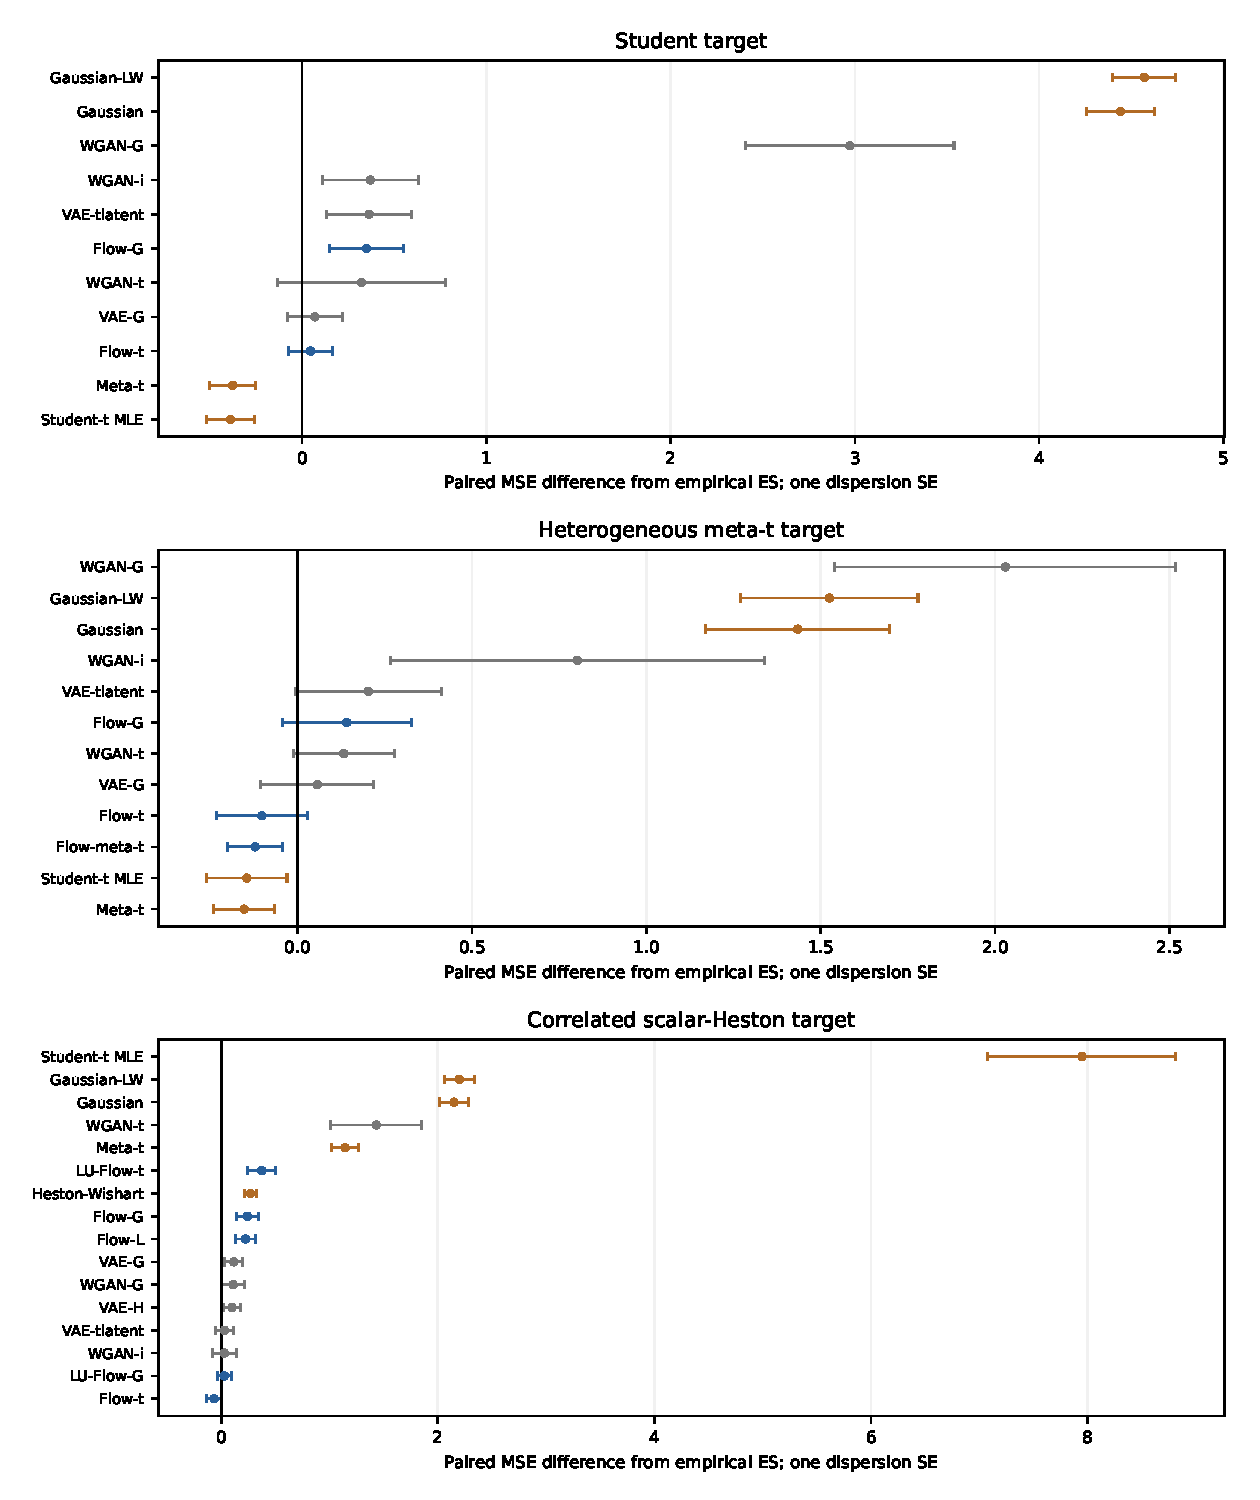
\includegraphics[width=0.98\linewidth]{wishart_paired_mse.pdf}\caption{One-percent ES MSE differences from exact empirical-training ES, with one dataset-level dispersion SE. Structured parametric laws, flows and other neural generators share estimation datasets.}\label{fig:r4-synthetic}\end{figure}
\FloatBarrier

\section{CRSP evidence: chronological tail-risk forecasting}\label{sec:crsp}
\subsection{Source audit and five size baskets}
The authorized CRSP CIZ daily extracts comprise 21 annual files for 2005--2025 and 40,402,817 security-day rows. Source SHA-256 digests are verified before constructing the expanded panel. The original audit checks year boundaries, required fields, and unique $(\mathrm{PERMNO},\mathrm{date})$ keys. It identifies 9,873 eligible historical securities and 5,282 five-basket return dates, January 4, 2005 through December 31, 2025.

Eligibility at formation close $s$ requires ordinary U.S. common equity: share type NS, security type EQTY, subtype COM, U.S.-incorporated flag Y, issuer type CORP or ACOR, primary exchange N/A/Q, regular-way conditional type RW, trading status A/H/S, and positive finite capitalization. Securities are sorted by capitalization, with PERMNO tie-breaking, into five approximately equal-count size baskets. For the immediately following trading date $t$,
\begin{equation}\label{eq:crsp-weights}
w_{i,b,t}=\frac{\operatorname{cap}_{i,s}\ind\{i\in\mathcal I_{b,s}\}}
{\sum_j\operatorname{cap}_{j,s}\ind\{j\in\mathcal I_{b,s}\}}.
\end{equation}
Returns are joined after holdings are formed. No return-date active-trading filter removes observed outcomes; 5,954 held observations with non-active return-date status and observed returns remain. CIZ total returns already incorporate the main-series delisting-return records, so no legacy delisting-return merge is added \citep{wrds2025ciz,crsp2025guide}. The extract lacks a separate daily delisting flag; non-active observations are not all called delistings.

Missing held returns receive an explicit zero-return convention, with a fixed-forecast $-20\%$ sensitivity for the 100-stock panel. In the size baskets, missing capitalization weight averages $5.21\times10^{-5}$ and reaches 0.00853. No return is winsorized. The equal combination of the five baskets is the primary portfolio; smallest- and largest-basket exposures are secondary. These are gross daily risk portfolios, not transaction-cost-adjusted investment strategies.

\subsection{An annually selected 100-stock panel}
For test year $y$, select the 100 largest eligible securities by capitalization at the last trading date of $y-2$, among securities with at least 98\% finite returns during the estimation window and at least 252 finite observations strictly before it. The pre-estimation history requirement prevents an IPO or cold-start return from being divided by an artificial near-zero volatility. The identities are fixed before the validation year $y-1$. No validation- or test-period availability, survival, return, or volatility criterion enters selection. Annual membership may change, but within a fold every model sees the same 100 securities, observations, and evaluation portfolios. The selected universes comprise established large-cap stocks.

Observed subsequent CIZ returns are retained even when trading status changes. Absent or missing entries are set to zero and supplied with a complete missingness mask. Consequently, a slot for a security that disappears can act as a zero-return allocation; the procedure does not retroactively replace it with a surviving security. This zero-return convention removes variation from missing slots and can bias downside-risk estimates downward, especially when missingness represents distress or unrecorded negative returns. The missing-return sensitivity is reported explicitly. The primary portfolio assigns weight $1/100$ to each slot. Secondary portfolios hold the ten largest formation-date stocks equally or the single largest stock. The dimension is 100 at estimation, while the number of active traded securities can subsequently be smaller. This convention makes the selection rule auditable and avoids a future-survivor screen.

\subsection{Predictable filters, annual fitting, and common selection}
Both panels use the predictable coordinate-volatility filter
\begin{equation}\label{eq:ewma-expanded}
\sigma_{i,t}^2=0.94\sigma_{i,t-1}^2+0.06R_{i,t-1}^2,
\qquad Z_{i,t}=R_{i,t}/\sigma_{i,t},
\end{equation}
initialized from the first 252 observations. The fixed daily decay follows \citet{riskmetrics1996}. Returns are in percentage points. Estimation excludes dates before 2006. For test year $y=2016,\ldots,2025$, estimation runs from $y-11$ through $y-2$, subject to that start date; $y-1$ is validation, and $y$ is test. Networks model multivariate innovations. No fitted parameter is updated inside a test year; the volatility state updates using information available at the preceding close.

Every neural family uses the common one-percent validation FZ0 rule in Section~\ref{sec:practice}. The five-basket study has two fresh optimization seeds per annual fold; the 100-stock extension has one. Each fitted generator supplies 100,000 innovation scenarios per fold, rescaled for each test date. The same scenarios are reused across dates to reduce simulation variation, without observing test returns. FHS evaluates the full empirical training innovation law exactly. The added joint Student and shrinkage-Gaussian laws contribute twenty model/fold records to each primary panel. The reproducibility ledger distinguishes records, optimizer seeds and replayed trajectories. Both panels have 2,514 test dates. 

\subsection{Dynamic statistical benchmarks}
In each panel, GARCH(1,1)-t is fitted separately to each evaluated portfolio with a constant mean, positive variance intercept, positive ARCH and GARCH coefficients summing to less than 0.9999, and $2.05\le\nu\le200$. Three numerical starts are used; the converged fit with the largest training likelihood is retained. Student innovations are normalized to variance one. The validation and test periods update states but do not re-estimate parameters. VaR and ES use analytic Student formulas.

The McNeil--Frey-style GARCH-EVT benchmark fits a generalized Pareto law to the upper five percent of training GARCH-standardized losses, then rescales its extrapolated quantile and ES by the predictable GARCH scale \citep{mcneil2000evt}. The specification is fixed across folds; all retained fitted shapes must have a finite mean. The POT implementation uses the fitted Student-GARCH filter.

EWMAcov-FHS updates the full second-moment matrix with decay 0.94, whitens each return by the predictable Cholesky factor, and recolors the empirical training innovations with the forecast-date factor. It therefore permits time-varying correlation. The ridge is $10^{-10}I$ in five dimensions and $10^{-8}I$ in 100 dimensions, in squared percentage-point units. In the 100-stock test states the minimum unregularized eigenvalue reaches $5.44\times10^{-13}$, so the ridge can dominate the weakest directions; the maximum regularized condition number is $4.64\times10^{10}$. This is a numerical floor rather than covariance shrinkage, and the small absolute ridge does not imply negligible whitening effects. With decay 0.94, the asymptotic weighting effective sample size is $(1+0.94)/(1-0.94)\simeq32.3$, so 100-dimensional covariance estimation can be noisy despite a long historical panel. This effective sample size is a weighting diagnostic, not an algebraic rank bound. Shrunk or factor covariance filters, including factor-DCC, remain relevant 100-stock controls beyond the evaluated full EWMA covariance. These diagnostics qualify the worse EWMAcov-FHS point scores; they do not identify their cause or establish a general cost of dynamic correlation. The 100-stock forecast has 14 exceedances (0.56\%), a Kupiec $p$-value of 0.015 and normalized ES moment $+0.156$ (Tables~\ref{tab:r4-crsp100-primary} and~\ref{tab:r4-calibration}); these outcomes do not isolate whitening noise as their cause. The empirical scenario law is enumerated, not resampled. Together these benchmarks distinguish conditional variance and correlation modeling.

An additional five-basket ablation refits the ten original specifications and the two added joint parametric benchmarks after full-covariance whitening, then recolors scenarios with each predictable forecast-date Cholesky factor. It uses seed zero, the same training budgets, validation FZ0, and 100,000 neural scenarios, giving 120 model/fold records. Paired comparisons use the corresponding diagonal-filter seed-zero forecasts. Twelve within-ablation Holm contrasts and a separate 2020 column distinguish conditioning effects from generator choice. 

\paragraph{Separating the variance filter from the residual tail.}
GARCH-FHS uses exactly the fitted portfolio GARCH-t mean, variance recursion, estimation dates, and subsequent predictable states, but replaces its parametric residual law by the full empirical training residual distribution. Portfolio-EWMA-FHS instead applies the zero-mean decay-0.94 filter directly to each portfolio loss and enumerates its empirical standardized residuals. Together with the two added joint parametric benchmarks, the primary comparison contains seventeen models and sixteen FHS contrasts. 

A further diagnostic portfolio-EWMA-FHS uses the fitted GARCH location, so the following daily score differences add exactly: multivariate FHS to portfolio-EWMA-FHS (aggregation and conditioning), introducing the GARCH location, changing only the variance recursion to GARCH, and replacing only the empirical residual tail by EVT. The final step isolates the incremental EVT contribution under a common fitted filter. A separate Student-versus-empirical comparison also holds the GARCH location and scale fixed. These six attribution contrasts have their own exploratory Holm adjustment. 

\paragraph{DCC and constant-correlation controls.}
The five-basket extension fits Gaussian and variance-normalized Student laws under constant correlation (CCC) and DCC, using the same estimated coordinate-GARCH scales \citep{engle2002dcc}. With standardized returns $z_t$, the recursion is
\[
Q_t=(1-a-b)\overline Q+a z_{t-1}z_{t-1}^{\top}+bQ_{t-1},\qquad
R_t=\operatorname{diag}(Q_t)^{-1/2}Q_t\operatorname{diag}(Q_t)^{-1/2}.
\]
Training likelihood estimates $a,b\ge0$, $a+b\le0.999$, and, for Student laws, $2.05\le\nu\le200$. Three DCC starts are used. The training second moment $\overline Q$ has a $10^{-10}I$ ridge; $Q_0=\overline Q$. CCC sets $a=b=0$. Parameters remain fixed during validation and testing; states update only after observations. Analytic portfolio risk eliminates scenario error for these four controls. Their eight contrasts against diagonal-EWMA-FHS and coordinate-GARCH-FHS form a retrospective family; a 21-model, 20-contrast encompassing sensitivity is archived separately. No high-dimensional DCC fit is included.


\subsection{Scores, paired inference, and calibration}
For realized loss $L_t$, VaR $q_t$, positive ES $e_t$, and tail probability $\alpha$, use
\begin{equation}\label{eq:fz}
S_\alpha(q_t,e_t;L_t)=\log e_t+q_t/e_t-1+
\frac{(L_t-q_t)_+}{\alpha e_t}.
\end{equation}
For a common positive unit conversion $c$, $S_\alpha(cq,ce;cL)=S_\alpha(q,e;L)+\log c$. Thus the percentage-point convention shifts all score levels by a common constant; paired score differences are invariant to that conversion. Levels are compared only for the same target and units, not across different portfolio laws. This is the loss-convention FZ0 score; lower is better \citep{fissler2016,patton2019}. Conditional calibration also implies zero conditional mean of
\begin{equation}\label{eq:es-moment}
m_t=e_t-q_t-(L_t-q_t)_+/\alpha,
\qquad \ind\{L_t>q_t\}-\alpha.
\end{equation}
The reported normalized ES moment is mean $m_t$ divided by $\overline e$; formal calibration tests are defined below.

The primary comparison in each panel is the equal-weight portfolio at one percent, with FHS as reference. For the five-basket panel, daily scores are averaged over the two seeds where available before time-series inference; deterministic or singly fitted benchmarks have one series. We use 9,999 paired circular block-bootstrap draws with block length 20 \citep{politis1992circular}. Averaging seed scores assesses typical fitted forecasts; it does not evaluate a mixture-of-scenarios or averaged-forecast ensemble a practitioner might use. For observed mean score difference $\widehat d$ and centered bootstrap error $Z^*=\widehat d^*-\widehat d$, report the basic interval
$[\widehat d-q_{.975}(Z^*),\widehat d-q_{.025}(Z^*)]$
and the matching two-sided, equal-tailed test at $\widehat d$, with a plus-one resampling correction. The primary set has seventeen models and sixteen contrasts against diagonal-EWMA FHS in each panel. Holm adjustment is applied \emph{within each panel} \citep{holm1979}. 

A 95\% model confidence set over seventeen specifications per panel uses the range statistic $T_R$ and elimination rule $e_R$ of \citet{hansen2011mcs}, with shared resamples and monotone elimination $p$-values. Block lengths 10 and 40 are sensitivity checks. Calibration uses integer exceedance sequences separately for each seed: Kupiec unconditional coverage \citep{kupiec1995} and a finite-instrument joint VaR--ES Wald diagnostic following \citet{nolde2017}. The latter stacks the two identification functions with instruments 1 and the previous hit deviation, using Bartlett HAC bandwidth 20 and a chi-square reference with covariance-rank degrees of freedom. 

The 2.5\% level, concentrated portfolios, 2020 exclusion, and exclusion of the 5, 10, or 20 largest realized losses are secondary diagnostics. Crash exclusions remove the same ex-post dates for every model. All bootstrap and calibration calculations condition on the fitted forecasts and do not refit models inside resamples. Interpretive limits are collected in Section~\ref{sec:limitations}.

\subsection{Five-basket results}
The lowest observed mean is GARCH-EVT at 1.3121, versus FHS 1.3700. None of the sixteen FHS contrasts establishes improvement after within-panel Holm adjustment. GARCH-EVT has difference -0.0578, interval $[-0.1090,-0.0037]$, and Holm $p=0.5550$. GARCH-FHS has difference -0.0524, interval $[-0.1031,-0.0008]$, and Holm $p=0.6328$. Student-$t$ MLE has difference -0.0008, interval $[-0.0666,0.0487]$, and Holm $p=1.0000$. The 95\% MCS retains 17 of seventeen models. Membership uses studentized pairwise differences and does not order retained forecasts by their sample means.
\begin{table}[htbp]
\centering\footnotesize
\setlength{\tabcolsep}{4pt}
\begin{tabular}{lrrrrrrr}
\toprule
Model & FZ0 & Hits \% & ES mom. & $\Delta$ FHS & 95\% interval & Holm $p$ & MCS $p$ \\
\midrule
GARCH-EVT & 1.312 & 1.03 & -0.023 & -0.058 & [-0.109, -0.004] & 0.555 & 1.000 \\
GARCH-FHS & 1.318 & 1.11 & -0.023 & -0.052 & [-0.103, -0.001] & 0.633 & 0.685 \\
Flow-meta-t & 1.335 & 1.01 & 0.006 & -0.035 & [-0.066, -0.008] & 0.106 & 0.698 \\
Flow-t & 1.335 & 1.21 & 0.019 & -0.034 & [-0.078, 0.008] & 1.000 & 0.698 \\
Flow-G & 1.346 & 1.27 & -0.112 & -0.024 & [-0.067, 0.012] & 1.000 & 0.698 \\
VAE-G & 1.346 & 1.21 & -0.132 & -0.023 & [-0.066, 0.012] & 1.000 & 0.698 \\
VAE-H & 1.347 & 1.21 & -0.134 & -0.022 & [-0.067, 0.015] & 1.000 & 0.698 \\
GARCH-t & 1.360 & 1.71 & -0.162 & -0.010 & [-0.093, 0.064] & 1.000 & 0.597 \\
Student-$t$ MLE & 1.369 & 1.39 & -0.089 & -0.001 & [-0.067, 0.049] & 1.000 & 0.685 \\
FHS & 1.370 & 0.95 & 0.026 & 0.000 & [0.000, 0.000] & 1.000 & 0.193 \\
WGAN-t & 1.373 & 1.33 & 0.171 & 0.003 & [-0.033, 0.041] & 1.000 & 0.209 \\
Port.-EWMA-FHS & 1.378 & 0.99 & 0.024 & 0.008 & [-0.004, 0.020] & 1.000 & 0.071 \\
EWMAcov-FHS & 1.379 & 0.91 & 0.024 & 0.009 & [-0.004, 0.023] & 1.000 & 0.076 \\
WGAN-G & 1.386 & 1.63 & -0.222 & 0.016 & [-0.076, 0.087] & 1.000 & 0.620 \\
Meta-t & 1.387 & 1.41 & -0.119 & 0.017 & [-0.058, 0.078] & 1.000 & 0.193 \\
Gaussian & 1.460 & 1.87 & -0.348 & 0.090 & [-0.057, 0.208] & 1.000 & 0.193 \\
Gaussian-LW & 1.460 & 1.83 & -0.347 & 0.090 & [-0.057, 0.209] & 1.000 & 0.193 \\
\bottomrule
\end{tabular}
\caption{5-coordinate equal-portfolio 1\% forecasts on 2,514 dates. Seventeen models, sixteen within-panel FHS contrasts. Neural candidates include initialization and early updates; Wishart CRSP is excluded. Basic intervals and matching tests use 9,999 circular resamples with 20-day blocks. MCS membership is not a ranking of retained models.}\label{tab:r4-crsp5-primary}
\end{table}

\subsection{100-stock results}
The lowest observed mean is GARCH-FHS at 1.1547, versus FHS 1.2692. Within-panel Holm adjustment detects an improvement only for Student-$t$ MLE. GARCH-EVT has difference -0.1120, interval $[-0.2259,0.0147]$, and Holm $p=1.0000$. GARCH-FHS has difference -0.1145, interval $[-0.2291,0.0124]$, and Holm $p=1.0000$. Student-$t$ MLE has difference -0.0230, interval $[-0.0410,-0.0077]$, and Holm $p=0.0352$. The 95\% MCS retains 17 of seventeen models. Membership uses studentized pairwise differences and does not order retained forecasts by their sample means.
The MCS uses an all-pairs statistic and sequential elimination rule, so it can retain FHS despite a significant contrast in the separately defined Holm family against that benchmark.
\begin{table}[htbp]
\centering\footnotesize
\setlength{\tabcolsep}{4pt}
\begin{tabular}{lrrrrrrr}
\toprule
Model & FZ0 & Hits \% & ES mom. & $\Delta$ FHS & 95\% interval & Holm $p$ & MCS $p$ \\
\midrule
GARCH-FHS & 1.155 & 0.91 & 0.013 & -0.115 & [-0.229, 0.012] & 1.000 & 1.000 \\
GARCH-EVT & 1.157 & 0.99 & 0.013 & -0.112 & [-0.226, 0.015] & 1.000 & 0.548 \\
GARCH-t & 1.184 & 1.43 & -0.082 & -0.085 & [-0.224, 0.054] & 1.000 & 0.548 \\
Student-$t$ MLE & 1.246 & 0.84 & -0.052 & -0.023 & [-0.041, -0.008] & 0.035 & 0.548 \\
Meta-t & 1.249 & 0.95 & -0.110 & -0.020 & [-0.070, 0.018] & 1.000 & 0.548 \\
FHS & 1.269 & 0.91 & -0.041 & 0.000 & [0.000, 0.000] & 1.000 & 0.113 \\
Port.-EWMA-FHS & 1.271 & 1.15 & 0.018 & 0.002 & [-0.134, 0.134] & 1.000 & 0.083 \\
EWMAcov-FHS & 1.285 & 0.56 & 0.156 & 0.016 & [-0.061, 0.126] & 1.000 & 0.131 \\
Flow-meta-t & 1.313 & 0.91 & -0.081 & 0.044 & [-0.029, 0.108] & 1.000 & 0.075 \\
WGAN-t & 1.314 & 1.23 & -0.032 & 0.045 & [-0.050, 0.127] & 1.000 & 0.400 \\
Gaussian-LW & 1.322 & 1.59 & -0.473 & 0.053 & [-0.125, 0.196] & 1.000 & 0.548 \\
Gaussian & 1.324 & 1.55 & -0.473 & 0.055 & [-0.124, 0.198] & 1.000 & 0.504 \\
Flow-t & 1.339 & 1.47 & -0.456 & 0.070 & [-0.112, 0.219] & 1.000 & 0.548 \\
VAE-H & 1.354 & 1.47 & -0.507 & 0.085 & [-0.148, 0.264] & 1.000 & 0.548 \\
Flow-G & 1.367 & 1.55 & -0.513 & 0.098 & [-0.126, 0.277] & 1.000 & 0.548 \\
WGAN-G & 1.373 & 1.75 & -0.571 & 0.104 & [-0.131, 0.299] & 1.000 & 0.548 \\
VAE-G & 1.377 & 1.51 & -0.524 & 0.107 & [-0.127, 0.297] & 1.000 & 0.548 \\
\bottomrule
\end{tabular}
\caption{100-coordinate equal-portfolio 1\% forecasts on 2,514 dates. Seventeen models, sixteen within-panel FHS contrasts. Neural candidates include initialization and early updates; Wishart CRSP is excluded. Basic intervals and matching tests use 9,999 circular resamples with 20-day blocks. MCS membership is not a ranking of retained models.}\label{tab:r4-crsp100-primary}
\end{table}

\paragraph{Conditioning and resolution.}
The portfolio-level decomposition holds location and residual scenarios fixed when changing the variance recursion. Its components still add exactly on each date. The incremental EVT effect is level-specific: the one-percent quantile lies inside an approximately 2,500-point innovation sample, where empirical interpolation remains possible. Undetected incremental EVT value here does not assess its extrapolation value at more extreme levels.
\begin{table}[htbp]
\centering\footnotesize
\setlength{\tabcolsep}{4pt}
\begin{tabular}{llrrr}
\toprule
Panel & Component & $\Delta$ FZ0 & 95\% interval & Holm/6 $p$ \\
\midrule
5 & Aggregation & 0.008 & [-0.004, 0.020] & 0.578 \\
5 & Location & -0.006 & [-0.017, 0.008] & 0.578 \\
5 & Variance filter & -0.055 & [-0.098, -0.013] & 0.072 \\
5 & EVT tail & -0.005 & [-0.013, 0.003] & 0.578 \\
5 & Total & -0.058 & [-0.109, -0.004] & 0.185 \\
5 & Student vs empirical & 0.043 & [-0.015, 0.095] & 0.578 \\
100 & Aggregation & 0.002 & [-0.134, 0.134] & 1.000 \\
100 & Location & -0.001 & [-0.018, 0.017] & 1.000 \\
100 & Variance filter & -0.115 & [-0.194, -0.025] & 0.096 \\
100 & EVT tail & 0.002 & [-0.002, 0.007] & 1.000 \\
100 & Total & -0.112 & [-0.226, 0.015] & 0.390 \\
100 & Student vs empirical & 0.029 & [-0.024, 0.077] & 1.000 \\
\bottomrule
\end{tabular}
\caption{Portfolio-filter attribution at one percent. The first four components sum exactly to Total on every date. Each panel has six exploratory contrasts. Student versus empirical holds the same fitted portfolio mean and GARCH variance fixed.}\label{tab:r4-filter}
\end{table}

The unadjusted interval half-widths for the GARCH/FHS contrasts are about 0.05 in five baskets and 0.12 in 100 stocks. Table~\ref{tab:r4-power} distinguishes this precision from conditional 80\%-power effects. Economically relevant differences can remain unresolved. The 2.5\% results are secondary; a future co-primary design requires advance specification.
\begin{table}[htbp]
\centering\footnotesize
\setlength{\tabcolsep}{4pt}
\begin{tabular}{llrrr}
\toprule
Panel & Contrast & CI half-width & MDE 80\% & MDE/16 \\
\midrule
5 & GARCH-FHS & 0.051 & 0.074 & 0.100 \\
5 & GARCH-EVT & 0.053 & 0.077 & 0.106 \\
100 & GARCH-FHS & 0.121 & 0.178 & 0.257 \\
100 & GARCH-EVT & 0.120 & 0.177 & 0.257 \\
\bottomrule
\end{tabular}
\caption{Conditional resolution diagnostic at one percent. MDE is the location shift giving 80\% power under retained bootstrap noise, with unadjusted 5\% or conservative sixteen-contrast Bonferroni thresholds. It does not simulate refitting or provide prospective power.}\label{tab:r4-power}
\end{table}

\begin{figure}[htbp]\centering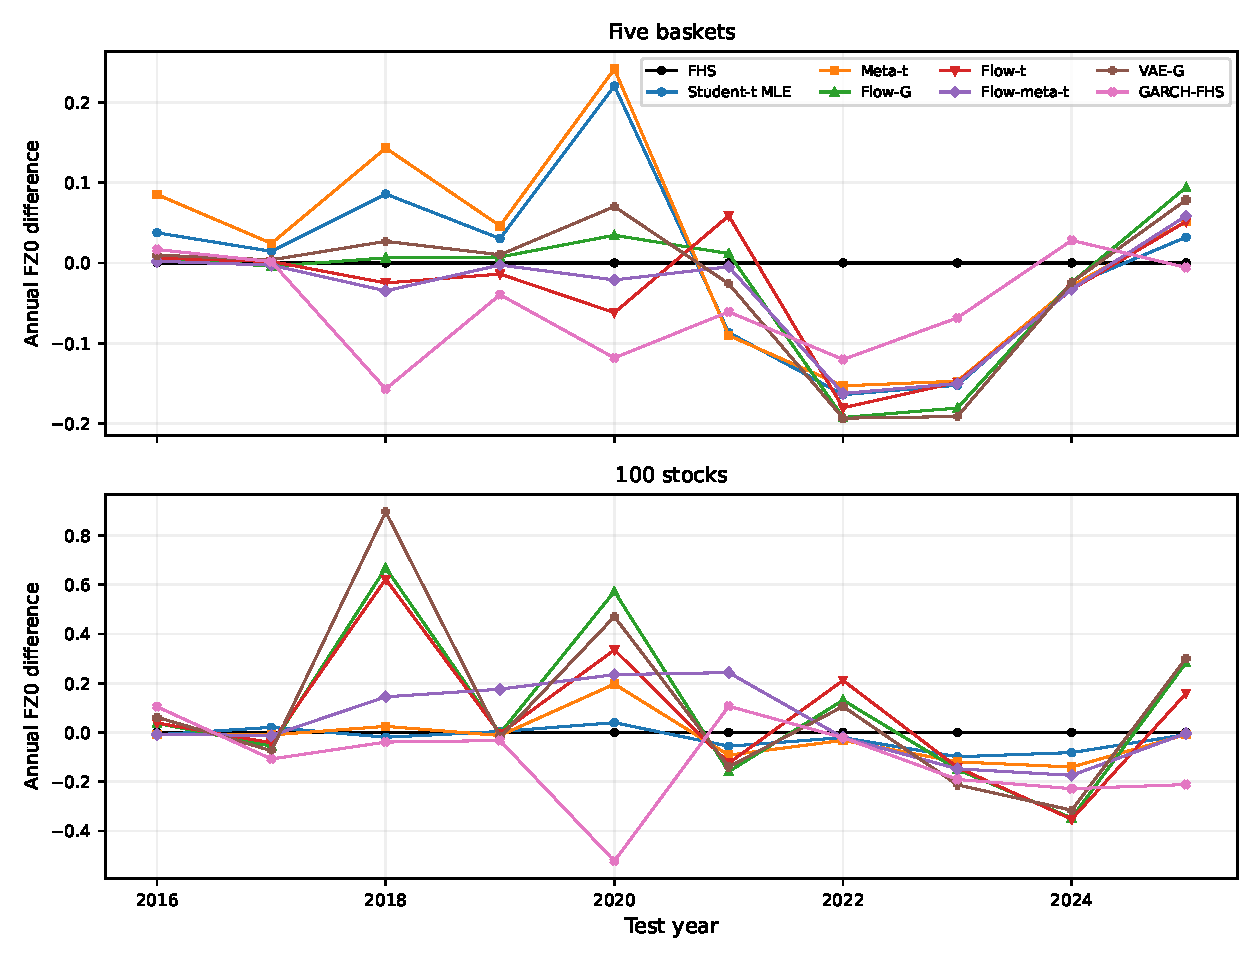
\includegraphics[width=0.98\linewidth]{round2_annual.pdf}\caption{Annual one-percent score differences from FHS under the stated selection. FHS is the zero reference. All model histories and primary seed conventions are retained in the accompanying records.}\label{fig:r4-annual}\end{figure}
\FloatBarrier

\section{Density, selection, and multivariate controls}\label{sec:checkpoint-results}
\subsection{Checkpoint selection and its sensitivity}\label{sec:checkpoint-repair}
The candidate grid contains initialization, updates $10,25,50,100$, and each 250th update thereafter. Flows also admit an identity coupling map; meta-$t$ residual flows admit the exact fitted base, and dense Gaussian and Student flows admit their fitted full-scatter parametric benchmarks. Every candidate is evaluated on the same validation observations and fixed scenario draws. Alternative rules use portfolio FZ0 at 2.5\% or 5\%, pooled-portfolio FZ0 at 1\%, likelihood, or the final state. Flows use exact validation NLL; VAEs use IWAE-8 for validation and IWAE-64 for testing. Table~\ref{tab:r4-selection} reports the matched comparison. The grid was amended during review to include omitted early and nested candidates before the new evaluations; replay and the excluded earlier comparisons are documented in the reproducibility audit. Test-period performance never selects a candidate under an individual rule.

Forty neural rule/model forecasts form one FHS comparison family per panel; the 33 alternatives against their own model's primary rule form another. The sensitivity uses seed zero, while the primary five-basket comparison averages two seed scores. A validation year contains only about 2.5 nominal one-percent exceedances.

\subsection{Paired density uncertainty}\label{sec:density-uncertainty}
Density tables evaluate the validation-likelihood-selected state on common test observations, including the initial and nested candidates. For CRSP, let $d_t=-\log q_m(X_t)+\log q_G(X_t)$, where $q_G$ is the full-covariance Gaussian under the same filter. We retain the pointwise differences, use the same 20-day circular bootstrap and basic intervals as for risk scores, and adjust the eight comparisons with Gaussian within each panel. The predictable filter Jacobian is included in every reported NLL and cancels in a same-filter paired difference. These calculations condition on the fitted forecasts and the realized sequence; they do not resample model estimation.

For synthetic law $p$, let $d_{ji}$ be the log-density difference for fitted dataset $j$ and common test observation $i$. We separately report
\[
 \mathrm{SE}_{\rm fit}=\frac{\operatorname{sd}_j(\overline d_{j\cdot})}{\sqrt{10}},
 \qquad
 \mathrm{SE}_{\rm test}=\frac{\operatorname{sd}_i(\overline d_{\cdot i})}{\sqrt{20{,}000}}.
\]
The first conditions on the shared test sample; the second conditions on the fitted models. They are descriptive components, not independent errors to add mechanically. In particular, quadratic log-density contrasts under a $t_3$ target can have infinite variance. The displayed empirical dispersion is therefore not promoted to a normal-theory confidence interval. VAE comparisons additionally retain the IWAE bias and Monte Carlo qualification from Section~\ref{sec:objectives}.

\subsection{Dense dependence and coordinate-filter controls}\label{sec:lu-controls}
Original Flow-G and Flow-t use identity base scatter and a diagonal output map; only Flow-t's degrees of freedom are learned. Bounded shifts exclude a general dense affine Gaussian map from that implementation. Flow-meta-$t$ instead starts with a fitted correlation matrix. These restrictions support the coordinate-index guarantee in Proposition~\ref{prop:marginal}, while limiting dependence representation. A dense map retains radial growth bounds but can mix heterogeneous marginal indices: dependence capacity and coordinate-level tail guarantees are different requirements.

The dense control appends $A=L_AU_A$, with a unit lower triangle and an upper triangle with positive exponential diagonal. Triangular solves give the inverse and the log determinant is the sum of the upper log diagonal \citep{kingma2018glow}. Its initial covariance factor is estimated from training observations. For a fixed nonsingular $A$, the radial bounds survive; arbitrary mixing can change heterogeneous coordinate indices. The diagonal and dense controls use matched training budgets and validation rules, with the nested candidates described above. This comparison changes capacity, initialization and available nested laws together. It evaluates the resulting specification rather than isolating one architectural coefficient.

For conditioning, a constant-mean GARCH(1,1)-$t$ is fitted to every coordinate using training data only. FHS, Gaussian, shrinkage Gaussian, multivariate Student, meta-$t$, and the three flows are fitted to the resulting joint innovations. A second FHS control estimates coordinate EWMA decay in $[0.8,0.9995]$ by training Gaussian quasi-likelihood. There are 1,050 GARCH and 1,050 EWMA scalar fits. Coordinate-GARCH with meta-$t$ innovations is a copula-GARCH benchmark: coordinate scales are dynamic, while its fitted Student margins and t copula are fixed within the year. Location and innovation estimation change along with filtering, so these comparisons complement the exact portfolio-level variance decomposition.

Nine original-filter/refit contrasts and seven innovation contrasts against coordinate-GARCH-FHS are adjusted separately within each panel. The dense head/rule study has six contrasts. A broader retrospective sensitivity combines the seventeen primary forecasts, two risk-selected dense flows, eight coordinate-GARCH models, and fitted-EWMA-FHS: 28 forecasts and 27 FHS contrasts. Its larger family is reported alongside the targeted comparisons.

\subsection{A joint downside-event diagnostic}\label{sec:joint-event}
To examine a feature of the joint law beyond the evaluated portfolios, each fold fixes the fifth percentile of each coordinate's training innovations. The held-out event is that at least two of five coordinates, or at least five of 100 coordinates, fall below those thresholds on the same date. Under the predictable diagonal filter, these define date-specific physical-return thresholds without using future observations.

Twelve innovation laws under the common diagonal-EWMA filter forecast this same event. FHS evaluates its probability exactly from the empirical innovation distribution. Scenario-based models reuse their 100,000 risk-evaluation scenarios; the two added analytic-risk benchmarks generate 100,000 draws for this diagnostic. With event indicator $Y_t$ and probability $p_t$, the Brier score is $(Y_t-p_t)^2$. Eleven FHS contrasts per panel use paired date-block inference. Full-covariance and GARCH conditioning remain separate controls; portfolio-specific GARCH benchmarks also provide no competing joint law. The event definition was fixed before computing these new scores, but the addition is retrospective relative to the main study. Because both the innovation law and innovation thresholds are fixed within a fold, $p_t$ is constant within that fold. This is a fold-level calibration check, not a test of within-year timing or dynamic discrimination. Appendix~\ref{app:dependence} retains it alongside the more direct pairwise check below.

\subsection{Finite-level pairwise downside calibration}\label{sec:pair-tail}
For each fitted t copula and pair $(i,j)$, compute
\[
\lambda_{L,ij}=2t_{\nu_c+1}\!\left(-\sqrt{\frac{(\nu_c+1)(1-P_{ij})}{1+P_{ij}}}\right),\qquad
\lambda_{ij}(u)=\frac{C_{ij}(u,u)}u,\quad u\in\{0.01,0.05\}.
\]
The first is the limiting tail coefficient \citep{demarta2005tcopula}; the second is a finite-level conditional exceedance probability. Numerical one-dimensional quadrature evaluates the latter, with a refinement check. Held-out indicators use training-fitted marginal quantiles. We average equally over pairs within each fold and then over dates, and bootstrap dates jointly across all pairs. This avoids treating 4,950 pairs as independent observations. We also report marginal exceedance rates: deviations in the joint statistic can reflect both copula and marginal error. The fitted model probabilities are also constant within each fold. Their additional value is pairwise calibration at a stated tail level, not within-year timing resolution; fitted marginal quantiles prevent a pure isolation of copula error. These descriptive intervals do not estimate a limiting coefficient from one-percent data.


\subsection{Results}\label{sec:control-results}
\paragraph{Selection sensitivity.}
Final states have lower observed one-percent scores than risk-selected states for 0 of seven models in 5 dimensions; final-minus-selected differences range from 0.0103 to 0.0577 (computed before rounding). Final states have lower observed one-percent scores than risk-selected states for 6 of seven models in 100 dimensions; final-minus-selected differences range from -0.107 to 0.063. For 100-stock Flow-meta-$t$, the mean is 1.3127 under risk selection and 1.2476 under likelihood selection, versus FHS 1.2692. The forty-contrast FHS and 33-contrast within-model adjustments are retained in the sensitivity records. These test-period comparisons diagnose rule sensitivity; they cannot choose a new primary rule without another evaluation sample.

\begin{table}[htbp]
\centering\footnotesize
\setlength{\tabcolsep}{4pt}
\begin{tabular}{llrrrr}
\toprule
Panel & Model & NLL & $\Delta$ Gaussian & 95\% interval & Holm $p$ \\
\midrule
5 & Meta-t & 3.863 & -0.201 & [-0.271, -0.113] & 0.002 \\
5 & Flow-meta-t & 3.874 & -0.190 & [-0.261, -0.102] & 0.002 \\
5 & Student-$t$ MLE & 3.877 & -0.186 & [-0.253, -0.103] & 0.002 \\
5 & Flow-t & 3.918 & -0.146 & [-0.219, -0.056] & 0.015 \\
5 & VAE-H & 3.961 & -0.103 & [-0.150, -0.043] & 0.015 \\
5 & VAE-G & 3.966 & -0.098 & [-0.144, -0.037] & 0.015 \\
5 & Flow-G & 3.977 & -0.086 & [-0.144, -0.018] & 0.030 \\
5 & Gaussian-LW & 4.057 & -0.007 & [-0.017, 0.004] & 0.189 \\
5 & Gaussian & 4.064 & 0.000 & [0.000, 0.000] & 1.000 \\
100 & Meta-t & 137.981 & -18.135 & [-20.025, -16.075] & 0.002 \\
100 & Flow-meta-t & 137.981 & -18.135 & [-20.025, -16.075] & 0.002 \\
100 & Student-$t$ MLE & 145.087 & -11.029 & [-12.504, -9.450] & 0.002 \\
100 & VAE-H & 147.407 & -8.709 & [-9.997, -7.332] & 0.002 \\
100 & VAE-G & 147.445 & -8.671 & [-9.963, -7.297] & 0.002 \\
100 & Flow-t & 152.854 & -3.262 & [-4.850, -1.548] & 0.002 \\
100 & Gaussian-LW & 155.999 & -0.117 & [-0.162, -0.069] & 0.002 \\
100 & Gaussian & 156.116 & 0.000 & [0.000, 0.000] & 1.000 \\
100 & Flow-G & 164.863 & 8.747 & [7.311, 10.152] & 0.002 \\
\bottomrule
\end{tabular}
\caption{Joint density comparison on common CRSP dates under likelihood selection, seed zero. Differences are from the full-covariance Gaussian. Basic intervals use 20-day paired blocks; eight comparisons with Gaussian are Holm-adjusted within each panel. VAE values are IWAE-64 estimates. These conditional intervals do not include retraining uncertainty.}\label{tab:r4-density}
\end{table}

\paragraph{Density results.}
In 5 dimensions, the lowest observed exact NLL is Meta-t at 3.863. In 100 dimensions, the lowest observed exact NLL is Meta-t at 137.981. The paired intervals quantify test-period precision conditional on fitted states. A low NLL does not select a calibrated portfolio forecast automatically. The identity and nested candidates make a failure to improve the base visible as a selection outcome.
In the 100-stock panel, likelihood validation selects the exact meta-$t$ identity residual in 10 of ten folds. Its NLL therefore reflects the fitted parametric base, not a learned residual improvement. The original Flow-t base has identity scatter; its likelihood-selected NLL is 152.854, versus Gaussian 156.116. Table~\ref{tab:r4-dense} separately reports dense-head likelihood levels and risk scores.

\FloatBarrier



\paragraph{Matched conditioning controls.}
In 5 dimensions, the targeted adjustments detect 0 improvements among nine filter/refit contrasts and 0 among seven innovation contrasts against common coordinate-GARCH-FHS. The broader 27-contrast comparison establishes 0 improvements over the original FHS. In 100 dimensions, the targeted adjustments detect 0 improvements among nine filter/refit contrasts and 0 among seven innovation contrasts against common coordinate-GARCH-FHS. The broader 27-contrast comparison establishes 0 improvements over the original FHS. These separately adjusted comparisons answer different questions; targeted significance does not transfer automatically to the broader family. Full-covariance conditioning, alternative rules and comparisons with portfolio-GARCH-FHS remain in the machine-readable sensitivity records.

\paragraph{Conventional dynamic-correlation controls.}
The observed means favor constant-correlation counterparts in all three five-basket comparisons: EWMAcov-FHS versus FHS (1.379 versus 1.370), DCC-G versus CCC-G (1.435 versus 1.423), and DCC-t versus CCC-t (1.349 versus 1.330). This point-score pattern does not establish a significant or general disadvantage of dynamic correlation. No improvement survives the eight-contrast adjustment against the two FHS filters. The primary-plus-DCC 21-model sensitivity likewise detects no improvement over FHS. These controls fill the conventional dynamic-correlation comparison in five dimensions; they do not identify all possible benefits of dynamic correlation. See Table~\ref{tab:r5-dcc}.

\FloatBarrier

\paragraph{Coverage and conditional calibration.}
Table~\ref{tab:r4-calibration} separates two diagnostics from the FZ0 comparisons. With the same portfolio-GARCH filter, the joint conditional-moment (CM) diagnostic rejects GARCH-FHS in both panels ($p<0.001$), whereas GARCH-EVT is not rejected ($p=0.271$ and $0.394$). This contrast accompanies no detectable incremental FZ0 gain from EVT. It suggests a role for residual-tail modeling in the tested calibration moments even when mean scores are unresolved. These are unadjusted, finite-instrument tests with sparse tail observations; different rejection outcomes neither establish full conditional calibration nor constitute a paired test that EVT improves it.

At the unadjusted 5\% threshold, Kupiec coverage rejects Gaussian, Gaussian-LW, GARCH-t and WGAN-G in both panels; GARCH-t has 1.71\% and 1.43\% exceedances. In five baskets, meta-$t$ is also rejected for one seed. In 100 stocks, Flow-G, Flow-t, VAE-G, VAE-H and EWMAcov-FHS are additionally rejected; EWMAcov-FHS has only 14 exceedances (0.56\%), against 25.14 expected. CM additionally rejects WGAN-t in both panels; VAE-G and VAE-H for seed zero and Gaussian for seed one in five baskets (the latter $p=0.0496$ before rounding); and EWMAcov-FHS, Flow-meta-$t$ and VAE-G in 100 stocks. FHS and GARCH-EVT are not rejected by either diagnostic in either panel. These calibration checks complement density and mean-score comparisons without changing their multiplicity-adjusted conclusions.


\paragraph{Finite-level dependence and fold-level calibration.}
The original co-exceedance probability is constant within each annual fold, so its Brier score assesses fold-level calibration rather than within-year timing. The pairwise model probabilities are likewise fold-constant; their different perspective is a pair-specific event at an explicit tail level. In 100 stocks the mean fitted limiting coefficient is 0.0027, while the mean model value $C_{ij}(0.05,0.05)/0.05$ is 0.212; the observed value is 0.240, with marginal exceedance rate 5.18\%. The observed-minus-model interval is $[-0.052,0.093]$. Thus a small limiting coefficient does not imply negligible finite-level joint downside risk. At 1\% in five baskets, the observed pairwise statistic is 0.859 versus 0.531 under the model, with a difference interval $[-0.134,0.704]$. There are 183 coordinate exceedances on 79 dates, including 41 dates with at least two; the average is 36.6 per coordinate, against 25.14 expected under nominal marginal calibration. The 1.46\% marginal exceedance rate can contribute to the joint discrepancy, so it cannot be attributed solely to the copula. All four pair-averaged difference intervals include zero; this limited resolution does not establish correct copula specification. Table~\ref{tab:r5-tail} reports both levels and panels, and Table~\ref{tab:r4-joint} retains the original event diagnostic.

\FloatBarrier
\section{Stochastic covariance: specification and numerical evidence}\label{sec:wc-results}
The restricted Wishart benchmark couples matrix admissibility to a narrow range of marginal dispersion. We test a constructive repair: $\Sigma_t=\eta W_t+(1-\eta)v_t C$, with an independent mean-one CIR variance factor $v$ and a Wishart matrix factor $W$. The matrix component permits correlation variation; the scalar factor supplies extra common variance dispersion. A market leverage channel preserves instantaneous covariance when switched off. Proposition~\ref{prop:wc-dispersion} proves the frozen-mixture kurtosis formula $6\eta^2/b+3(1-\eta)^2/a$, which can match the Heston reference without violating the matrix condition. Appendix~\ref{app:wishart-cir} states the dynamics, estimator, simulation and filter. This retrospective specification experiment uses the same Heston estimation datasets. Its synthetic results and numerical diagnostics are reported separately from the primary conditional comparisons and their multiplicity families.

\paragraph{Tail dispersion is repaired; portfolio specification remains important.}
Across the ten Heston training datasets, mean fitted marginal excess kurtosis is 3.169 against 3.168 observed. The full extension's one-percent ES RMSE is 0.597, compared with 0.628 for restricted Wishart and 0.352 for empirical ES. The paired MSE change from restricted Wishart is $-0.038$ with dataset SE 0.083, so that improvement is unresolved. At 0.1\%, its RMSE rises to 1.543, versus 1.261 and 1.009 respectively. Matching marginal dispersion therefore does not establish better portfolio-tail estimation. Proposition~\ref{prop:wc-equivalence} strengthens this point: the frozen stationary return law is exactly a scalar Gaussian variance mixture, so static density or marginal-tail fit cannot identify the benefit of stochastic correlation. Every frozen portfolio has the same normalized kurtosis, and the frozen cross-asset squared-return moment is constrained by correlation and kurtosis alone (\ref{eq:wc-cross-moment}). The finite-day fitted cross-asset moment averages 2.069 against 1.535 observed. This supports excessive common variance concentration as a remaining specification problem, without uniquely attributing the finite-horizon ES error to it.
\begin{table}[htbp]
\centering\small
\begin{tabular}{lrrrr}
\toprule
 & \multicolumn{2}{c}{1\% weekly ES} & \multicolumn{2}{c}{0.1\% weekly ES} \\
Model/intervention & RMSE & $\Delta$MSE (SE) & RMSE & $\Delta$MSE (SE) \\
\midrule
Empirical & 0.352 & +0.000 (0.000) & 1.009 & +0.000 (0.000) \\
Restricted Wishart & 0.628 & +0.271 (0.056) & 1.261 & +0.573 (0.288) \\
Wishart--CIR & 0.597 & +0.233 (0.054) & 1.543 & +1.364 (0.368) \\
Same fit, no scalar leverage & 0.136 & -0.106 (0.050) & 0.385 & -0.869 (0.295) \\
Same fit, fixed component correlation & 0.572 & +0.203 (0.053) & 1.522 & +1.301 (0.364) \\
\bottomrule
\end{tabular}
\caption{Retrospective Wishart--CIR extension on the same ten Heston estimation datasets. $\Delta$MSE is paired against the empirical estimator; SE reflects variation across the ten datasets, conditional on the shared reference sample. The two interventions reuse the fitted parameters and paths and are not separately selected models. All stochastic-covariance rows use 32 substeps and 131,072 conditional Gaussian paths per fit.}\label{tab:wc-synthetic}
\end{table}


\paragraph{Matched interventions identify the model's sensitivities.}
Removing scalar leverage from the same fitted paths reduces mean one-percent ES by 0.670 and RMSE to 0.136. At 0.1\%, RMSE becomes 0.385. These are useful mechanism diagnostics, not a new validation-selected winner: the Heston target itself has leverage, and the smaller error can compensate for other misspecification. By comparison, fixing only the Wishart component's correlation reduces mean one-percent ES by 0.026 and leaves RMSE at 0.572. Of these interventions, the common leverage channel has the larger effect. The correlation intervention preserves marginal variance paths, but changes mean off-diagonal covariance and leaves total correlation variable. It therefore does not isolate stochastic correlation at fixed average covariance or establish a forecasting benefit. Table~\ref{tab:wc-synthetic} reports paired errors, including the favorable ablation, without selecting a model after observing those errors.

\paragraph{Numerical eligibility for conditional comparison.}
The completed audit retains thirty filter runs. Finer 2020 checks pass, but the 2025 fold fails: at 32,768 particles the guided filter has 4.40\% independent-bank ES discrepancy, and the final 16,384-particle resample-move control has 6.13\% against a 2\% tolerance. Appendix~\ref{app:wishart-cir} reports the proposal correction, invariant refresh and failed refinements. The numerical gate excludes Wishart--CIR from the conditional CRSP comparison and from its Holm and MCS families. Its evidence consists of the stated mathematical results, synthetic specification experiment and numerical failure diagnostics. A full-panel forecast score or an allocation claim would exceed that evidence.

\FloatBarrier

\section{Implications and limitations}\label{sec:limitations}
The strongest observed filter effects prioritize volatility conditioning in this design, but their adjusted tests remain inconclusive. The neural conclusion concerns small bounded architectures for static innovations and a fixed training budget. Dense-output controls admit their nested parametric laws; they do not exhaust wider networks, unbounded shifts, alternate objectives or recursive conditional generators. The five-basket DCC extension supplies a conventional dynamic-correlation control; no 100-stock DCC evaluation is claimed. Coordinate-GARCH/meta-$t$ supplies a static-copula GARCH control in both panels.

Each checkpoint rule uses validation observations only. The candidate grid was amended retrospectively, before the associated new evaluations, to include initialization, early states and admissible nested laws. Selecting a different rule after inspecting its test performance still requires independent confirmation. One-percent validation contains about 2.5 nominal exceedances per CRSP year; pooled portfolios add exposures rather than independent dates. The 100-stock panel has one optimization seed, so its between-seed training variation is unmeasured.

Inference conditions on retained forecasts. Date-block resampling preserves cross-model pairing but does not refit models, regenerate scenarios, or establish equivalence. The Holm families in Table~\ref{tab:r4-families} have separate scopes; there is no global error guarantee over the retrospective research exercise. MCS membership depends on studentized pairwise precision and the candidate set, rather than ordering every retained model above every excluded one. Seed-score averaging measures typical fitted forecasts; an ensemble of forecasts would need its own evaluation.

Established large-cap universes, zero-filled missing allocations and a small set of portfolio exposures limit external validity. Missing distress returns can suppress measured downside risk. The partial fixed-forecast stress and complete-date diagnostics cannot recover those outcomes. In 100 stocks, GARCH-FHS minus FHS is $-0.115$ at baseline, $-0.023$ under the 20\% missing-return stress and $-0.163$ on complete dates; its sign persists in these diagnostics, but its magnitude depends on the convention. Portfolio-EWMA-FHS moves from $+0.002$ to $+0.289$ under the same stress (Table~\ref{tab:missing100}). The original co-exceedance score measures fold-level joint-event calibration, with constant probabilities inside a fold. Pairwise model probabilities are also fold-constant; these diagnostics separate asymptotic tail coefficients from finite-level joint exceedances, without adding timing resolution; their uncertainty still includes marginal-calibration error and only 2,514 dates.

Synthetic results condition on ten estimation datasets, and Heston on a finite joint variance bank and time discretization. Heavy tails limit normal-theory interpretations of squared-error SEs. The restricted Wishart fit understates synthetic risk; its CRSP filter fails the declared numerical tolerance and remains excluded from primary scores, Holm families and MCS. Neither finding rejects the general Wishart family or identifies the incremental benefit of stochastic correlation. The additive extension relaxes the dispersion restriction, but its synthetic results remain sensitive to the common leverage specification (Section~\ref{sec:wc-results}).

% BEGIN allocation-scope
\paragraph{Implications for portfolio modeling.}
These experiments evaluate predeclared portfolios, not weights optimized against each fitted law. Parametric meta-$t$ and its residual flow are tractable candidates for joint scenario modeling, but the likelihood-selected residual is the exact parametric identity in every 100-stock fold. The present evidence therefore establishes no advantage from that learned residual. For allocation, a separate chronological experiment must estimate weights using past information, impose common constraints and costs, and compare realized portfolio outcomes. Density or fixed-portfolio ES rankings alone do not validate an optimization policy.
% END allocation-scope

\section{Conclusion}
The comparison yields different answers for density estimation and portfolio forecasting. Meta-$t$ has the best observed exact density fit in both CRSP panels. In 100 stocks, likelihood validation selects the parametric identity in all ten residual-flow folds, so that result supplies no evidence of improvement from the learned residual. Under the common one-percent checkpoint rule, none of the tested neural innovation models establishes an adjusted FZ0 improvement over FHS. Student improves in the primary 100-stock family (Holm $p=0.0352$), while its broader-family result ($p=0.0594$) shows the sensitivity to the inferential scope. Checkpoint alternatives materially change rankings.

Changing the portfolio variance recursion accounts for the largest observed score gains: approximately $-0.055$ in five baskets and $-0.115$ in 100 stocks. Their adjusted tests remain inconclusive. EVT supplies no detectable incremental FZ0 gain at one percent; the differing conditional-moment outcomes for GARCH-FHS and GARCH-EVT concern the tested calibration restrictions and do not establish a significant paired improvement. Thus conditioning is the leading point-score explanation in this design, with finite-sample uncertainty applying equally to statistical and neural models.

The synthetic experiments show why specification and the evaluation level matter. Parametric models benefit when their family contains the target. Under Heston misspecification, a better fitted density can accompany substantially worse ES, and favorable one-percent errors can deteriorate at 0.1 percent. The Wishart--CIR construction removes the restricted model's marginal-dispersion ceiling, yet matching kurtosis leaves joint-risk errors and leverage sensitivity. Its frozen-law equivalence also prevents static density fit from identifying a benefit of stochastic correlation. Both evaluated Wishart filters fail their numerical gates and are excluded from conditional ranking.

These findings apply to the stated architectures, samples, portfolios and retrospective comparison design. They support a practical order of assessment: establish numerically stable forecasts, compare predictable conditioning, then test whether a more flexible joint law improves the specified density, dependence or risk objective under a fixed validation procedure. A model's likelihood ranking alone cannot answer the portfolio-risk question, and fixed-exposure forecasts do not validate optimized portfolio weights.

\appendix
\section{Proofs of the architectural results}\label{app:proofs}
\paragraph{Proof of result~\ref{thm:growth}.}
\begin{proof}
The upper and lower bounds follow from event inclusions. Dividing logarithms in \eqref{eq:sandwich} by $\log r$ proves preservation of the logarithmic index. To obtain the converse, invert the argument changes in the same inequalities to sandwich $\Prob(\|Z\|>r)$ between two affine rescalings of the output survival function. The moment equivalence follows directly from the two growth inequalities and $(a+b)^k\le C_k(a^k+b^k)$ for nonnegative $a,b$. For Gaussian $Z\in\R^m$, $\log\Prob(\|Z\|>r)=-r^2/2+O(\log r)$. Substitution gives two strictly negative finite quadratic-rate bounds.
\end{proof}

\paragraph{Proof of result~\ref{cor:coupling}.}
\begin{proof}
For each input, write the map as $A(z)z+b(z)$, where $A(z)$ is diagonal with entries in $[e^{-\bar s},e^{\bar s}]$ (including unchanged entries equal to 1), and $\|b(z)\|\le\sqrt d\bar t$. Upper and reverse triangle inequalities give the result. Composition preserves the inequalities, and an invertible affine map has positive minimum and finite maximum singular values.
\end{proof}

\paragraph{Proof of result~\ref{prop:marginal}.}
\begin{proof}
For an updated coordinate, $e^{-\bar s}|z_i|-\bar t\le|x_i|\le e^{\bar s}|z_i|+\bar t$; other coordinates are unchanged. Compose these coordinatewise inequalities and track permutations. The scalar version of the proof of Theorem~\ref{thm:growth} applies. To see why norm control is insufficient, let $H$ and $K$ be independent heavy-tailed variables of distinct indices and use the invertible linear map $(H,K)\mapsto(H,H+K)$. The norm index is preserved while the lighter coordinate can inherit the heavier index.
\end{proof}

\paragraph{Proof of result~\ref{prop:bounded-vae}.}
\begin{proof}
The event $|X_i|>r$ requires $\bar\sigma|\eta_i|>r-M$. For a lower bound, intersect $\{\sigma_i\ge a\}$ with $\{|\eta_i|>(r+M)/a\}$; the events are independent and imply $|X_i|>r$. Gaussian upper and lower logarithmic asymptotics complete the proof. Without nondegeneracy, for example $\sigma_i\equiv0$, the output can instead be bounded.
\end{proof}

\paragraph{Proof of result~\ref{thm:scale}.}
\begin{proof}
Put $t=r^{1/(\beta+1)}$. If $\|Z\|\le at$ and $|\eta|\le bt$, then for suitably small fixed positive $a,b$ and large $r$, $|X|\le r$. Thus the survival probability is bounded above by a sum of two Gaussian tails at thresholds proportional to $t$, giving $\log\Prob(|X|>r)\le-c_1t^2$. For a lower bound, restrict $Z$ to a fixed smaller cone and to $at\le\|Z\|\le2at$, and require $|\eta|>bt$, with $ca^\beta b>1$ and enough slack for $M$. The bounded location $\mu$ cannot cancel this growing scale-noise product on the cone. Independence and Gaussian shell probabilities give $\log\Prob(|X|>r)\ge-c_2t^2$. For the exponential scale upper bound, split at $\|Z\|=(\log r)/(2C)$ and $|\eta|$ proportional to $\sqrt r$. For the lower bound, restrict $Z$ to a cone and a shell at radius proportional to $\log r$ and take $|\eta|$ in a fixed interval bounded away from zero.
\end{proof}

\paragraph{Proof of result~\ref{prop:gan}.}
\begin{proof}
The growth bound follows from Lipschitz continuity at zero. Gaussian concentration gives
$\log\E e^{\lambda(L-\E L)}\le\lambda^2K_G^2\|w\|^2/2$ \citep{boucheron2013}. Each admissible density $\zeta$ in \eqref{eq:dual} defines $Q$ with $\KL(Q\|P)\le\log(1/\alpha)$. The entropy variational inequality gives
$\E_Q L-\E L\le\lambda K_G^2\|w\|^2/2+\log(1/\alpha)/\lambda$.
Minimize over $\lambda>0$ and take the supremum over $Q$.
\end{proof}

\paragraph{Proof of result~\ref{thm:shared}.}
\begin{proof}
Lipschitz continuity and positive homogeneity of the activations imply, by induction over layers, a finite $B$ with $\sup_z\|G(z)-G_0(z)\|\le B$ and $G_0(rz)=rG_0(z)$ for $r\ge0$. Thus the loss differs from $Rh(U)$ by at most $\|w\|B$. Continuity and compactness make $h(U)_+$ bounded. When its $\nu$th moment is positive, Breiman's lemma gives \eqref{eq:one-sided-relu}; bounded additive perturbations leave a regularly varying survival asymptote unchanged. If the moment is zero, continuity and the full spherical support imply $h\le0$, so the loss is bounded above by $\|w\|B$. Applying the argument to both signs of a coordinate gives the last statement.
\end{proof}

\paragraph{Proof of result~\ref{prop:independent}.}
\begin{proof}
Use $\min(a,b)=a-(a-b)_+$ for nonnegative $a,b$; an identity coordinate is the difference of two ReLUs. Independence gives $\Prob(G_2(Z)>r)=\Prob(Z_1>r)\Prob(Z_2>r)\sim k_\nu^2r^{-2\nu}$. The first coordinate has its original index.
\end{proof}

\paragraph{Proof of result~\ref{prop:meta}.}
\begin{proof}
Differentiate $F_{\nu_i}(T_i(y))=F_{\nu_c}(y)$ to obtain $T_i'=f_{\nu_c}/(f_{\nu_i}\circ T_i)$. The Student density satisfies
$f_\nu(y)\sim\Gamma((\nu+1)/2)\nu^{\nu/2}y^{-\nu-1}/(\sqrt\pi\Gamma(\nu/2))$.
Integrating divides the leading constant by $\nu$, giving \eqref{eq:constant}. Equate $k_{\nu_i}T_i(y)^{-\nu_i}$ with $k_{\nu_c}y^{-\nu_c}$ to obtain \eqref{eq:meta-asymptote}. Along each coordinate axis, an exponent above one violates a linear upper bound and an exponent below one violates a positive linear lower bound. If every exponent equals one, $T_i$ is the identity and the remaining scaling and translation are affine.
\end{proof}

\paragraph{Proof of result~\ref{prop:residual}.}
\begin{proof}
Proposition~\ref{prop:marginal} gives marginal index $\nu_c$ for every $\widetilde Y_i$, regardless of a final permutation because all base-coordinate indices coincide. The inverse of the regularly growing map in \eqref{eq:meta-asymptote} grows with exponent $\nu_i/\nu_c$, so substitution in the logarithmic survival limit yields index $\nu_i$. Change of variables gives the composed density. Exact marginal quantile calibration would require $F_{\nu_c}(\widetilde Y_i)$ to be uniform, which arbitrary residual coupling does not enforce. Coordinatewise monotone output maps preserve the residual's copula, not necessarily the original base copula.
\end{proof}
\section{Objective bounds and radial tail calibration}\label{sec:certificates}
\begin{theorem}[Sharp Wasserstein--ES continuity]\label{thm:w1}
For integrable real loss laws $P,Q$,
\begin{equation}\label{eq:w1-es}
|\ES_\alpha(P)-\ES_\alpha(Q)|\le\Wone(P,Q)/\alpha.
\end{equation}
For any integrable $P$, $\alpha\in(0,1)$, and $\varepsilon>0$, equality is attainable with $\Wone(P,Q)=\varepsilon$. For vector returns, the right-hand side is at most $\|w\|\Wone(P_X,Q_X)/\alpha$.
\end{theorem}
\begin{proof}
Apply the triangle inequality to \eqref{eq:es}, extend the resulting absolute-quantile integral to $[0,1]$, and use the one-dimensional Wasserstein identity. For sharpness, set $F_Q^{-1}(u)=F_P^{-1}(u)+(\varepsilon/\alpha)\ind\{u>1-\alpha\}$. This is nondecreasing and has the asserted transport cost and ES change. The portfolio bound follows by pushing a coupling through the $\|w\|$-Lipschitz projection.
\end{proof}
This is a standard Wasserstein risk-continuity fact, consistent with the distributionally robust formulation of \citet{esfahani2018}; it is included with a sharp construction for completeness. A certified upper bound on $\Wone$ can certify ES, but a bound large relative to $\alpha$ is uninformative. A trained critic value is not such an upper bound.

\begin{proposition}[Forward KL has no unrestricted ES modulus]\label{prop:kl}
For any integrable $P$, $\alpha\in(0,1)$, $\varepsilon>0$, and $K>0$, there is an integrable $Q$ with $\KL(P\|Q)\le\varepsilon$ and $\ES_\alpha(Q)\ge\ES_\alpha(P)+K$.
\end{proposition}
\begin{proof}
Choose $0<\omega\le\min(\alpha/2,1-e^{-\varepsilon})$ and $Q=(1-\omega)P+\omega\delta_M$. Since $Q\ge(1-\omega)P$, $\KL(P\|Q)\le-\log(1-\omega)$. On the mixture probability space, choose $\zeta=1/\alpha$ on the added component and $\zeta=(\alpha-\omega)/(\alpha(1-\omega))$ on the original component. This is feasible in \eqref{eq:dual}, so
$\ES_\alpha(Q)\ge\omega M/\alpha+(\alpha-\omega)\E_P L/\alpha$.
Let $M$ be sufficiently large. The same obstruction can be made absolutely continuous by replacing the atom with a bounded-width density translated to $M$.
\end{proof}

\begin{proposition}[Finite likelihood cost and a slowly varying factor]\label{prop:finite-kl}
Suppose $p\le p_{\max}$, $\E_p\|X\|^2<\infty$, and $q(x)\ge c_0e^{-b\|x\|^2}$ for positive constants. Then $\KL(p\|q)<\infty$ and
\begin{equation}\label{eq:kl-tail}
\int_{\|x\|>r}p\log(p/q)\,dx
\le A\Prob_p(\|X\|>r)+b\E_p[\|X\|^2\ind\{\|X\|>r\}],
\end{equation}
where $A=\log^+(p_{\max}/c_0)$. If $\Prob(\|X\|>r)=r^{-\nu}\ell(r)$ with $\nu>2$, the upper bound is $O(r^{2-\nu}\ell(r))$.
\end{proposition}
\begin{proof}
The pointwise upper bound is $\log(p/q)\le\log(p_{\max}/c_0)+b\|x\|^2$. Integrating gives \eqref{eq:kl-tail} and integrability of the positive part. The negative part of relative entropy is integrable, using $t\log(1/t)\le1/e$ under $q$. Karamata's theorem gives
$\E[\|X\|^2\ind\{\|X\|>r\}]\sim\nu r^2\Prob(\|X\|>r)/(\nu-2)$ \citep{embrechts1997}.
\end{proof}
The slowly varying factor cannot generally be omitted. The lower bound on $q$ does not prove divergence when the second moment is infinite: a heavy-tailed $q=p$ can satisfy that lower bound and have zero KL. If instead $q\le Ce^{-b\|x\|^2}$ and $\int p|\log p|<\infty$, an infinite second moment does imply infinite KL. At index $\nu=2$, moment existence depends on $\ell$. These are population statements. Finite-sample Gaussian likelihoods remain finite, and finite population KL does not make likelihood intrinsically unable to estimate a tail parameter in a suitably specified family.

\subsection{Radial EVT calibration with angular conditions}\label{sec:repair}
Let $\widetilde X=\widetilde R\widetilde\Theta$ be generated samples with a continuous radius law and negligible mass at the origin. Set $U=F_{\widetilde R}(\widetilde R)$. A radial transplant defines
\begin{equation}\label{eq:transplant}
X'=H(U)\widetilde\Theta,
\end{equation}
where $H$ is the quantile function of an empirical body up to threshold $u$ and a generalized Pareto excess law above it. With tail mass $q_0$, the upper branch is
$H(v)=u+G^{-1}_{\xi,\beta}((v-1+q_0)/q_0)$ for $v>1-q_0$.
Finite samples use mid-ranks; this discretized sampler approximates the population construction.

\begin{proposition}[Radial calibration and portfolio tails]\label{prop:transplant}
The radius of \eqref{eq:transplant} has quantile function $H$, and the direction and its association with the original rank $U$ are unchanged. Suppose $\xi>0$, $\kappa=1/\xi$, and, conditionally on $A=\{U>1-q_0\}$, direction is independent of $U$. If $\Prob(-w^\top\widetilde\Theta>\eta\mid A)>0$ for some $\eta>0$, then
\begin{equation}\label{eq:breiman}
\Prob(-w^\top X'>x)\sim
\E[((-w^\top\widetilde\Theta)_+)^\kappa\mid A]\Prob(H(U)>x).
\end{equation}
The portfolio upper tail has index $\kappa$; finite upper-tail ES requires $\kappa>1$, equivalently $\xi<1$.
\end{proposition}
\begin{proof}
The probability integral transform makes $U$ uniform. Equation~\eqref{eq:transplant} changes radius but retains $(U,\widetilde\Theta)$, which establishes the first claims. For sufficiently large losses only $A$ contributes. Conditional independence on $A$, boundedness of $(-w^\top\widetilde\Theta)_+$ by $\|w\|$, and Breiman's lemma give the conditional tail equivalence. Multiplying by $\Prob(A)=q_0$ converts the conditional radial survival function into the unconditional one. The angular coefficient is positive by hypothesis. GPD moment existence gives the ES condition.
\end{proof}
The expectation in \eqref{eq:breiman} is conditional on the tail region. An empirical-body quantile map need not be strictly increasing, so a claim of exact preservation of a continuous radius-direction copula after introducing atoms would be too strong. Asset-coordinate copulas are not generally preserved. Moreover, Euclidean radius and direction are not independent for a general elliptical law; whitening gives the spherical representation where independence is exact, while asymptotic angular convergence can justify separate extreme-limit statements. Heterogeneous margins can induce radius-dependent angular concentration. A radial repair can then improve one portfolio and worsen another. It calibrates a radial distribution; it does not universally remove architecture or angular error.

\section{Stochastic volatility and the Heston distinction}\label{sec:heston}
For scalar Heston log returns,
\begin{equation}\label{eq:heston}
dV_t=\kappa(\theta-V_t)dt+\xi\sqrt{V_t}\,dB_t,\quad
dR_t=-\tfrac12V_tdt+\sqrt{V_t}\,dW_t,\quad d\langle B,W\rangle_t=\rho\,dt.
\end{equation}
The CIR stationary variance margin is gamma with shape $a=2\kappa\theta/\xi^2$ and scale $b=\theta/a$. All parameters are positive and $|\rho|<1$ below.

\begin{proposition}[Frozen-variance snapshot]\label{prop:frozen}
Let $V\sim\Gamma(a,b)$ be independent of $N\sim N(0,1)$. For $R_0=\sqrt{V\Delta}N$,
\begin{equation}
M_{R_0}(u)=(1-b\Delta u^2/2)^{-a},\quad
\lim_{r\to\infty}-r^{-1}\log\Prob(|R_0|>r)=\sqrt{2/(b\Delta)}.
\end{equation}
For $R_d=-V\Delta/2+\sqrt{V\Delta}N$, the MGF is $[1-b\Delta(u^2-u)/2]^{-a}$, with endpoints
$u_\pm=(1\pm\sqrt{1+8/(b\Delta)})/2$. Its right and left logarithmic tail rates are $u_+$ and $-u_-$.
\end{proposition}
\begin{proof}
Condition on $V$ and use the gamma Laplace transform. For $R_0$, integrating the normal density against the gamma density gives a constant multiple of
$|r|^{a-1/2}K_{a-1/2}(|r|\sqrt{2/(b\Delta)})$.
The asymptote $K_\eta(x)\sim\sqrt{\pi/(2x)}e^{-x}$ gives the stated rate and a density prefactor proportional to $|r|^{a-1}$. For $R_d$, completing the square in the normal-gamma integral adds the exponential tilt $e^{-r/2}$ and changes the Bessel rate to $\sqrt{1/4+2/(b\Delta)}$, giving the two roots. These are variance-gamma mixtures \citep{madan1990vg}, not the full Heston transition law.
\end{proof}

\begin{proposition}[Exact Heston mixture and transform]\label{prop:heston-transform}
Put $I_T=\int_0^TV_sds$. There is $N\sim N(0,1)$ independent of the variance path such that, in distribution jointly with that path,
\begin{equation}\label{eq:heston-mixture}
R_T=-\tfrac12I_T+\frac{\rho}{\xi}(V_T-V_0-\kappa\theta T+\kappa I_T)
+\sqrt{1-\rho^2}\sqrt{I_T}N.
\end{equation}
For deterministic $V_0=v$, the MGF on its domain of finiteness is $e^{C(T,u)+D(T,u)v}$, with
\begin{equation}\label{eq:riccati}
\partial_tD=\tfrac12\xi^2D^2+(\rho\xi u-\kappa)D+\tfrac12(u^2-u),\qquad
\partial_tC=\kappa\theta D,\quad C(0,u)=D(0,u)=0.
\end{equation}
If $V_0\sim\Gamma(a,b)$ independently of future Brownian increments, then
$M_R(u)=e^{C(T,u)}(1-bD(T,u))^{-a}$ whenever the Riccati solution remains finite and $bD(T,u)<1$.
\end{proposition}
\begin{proof}
Decompose $W=\rho B+\sqrt{1-\rho^2}B^\perp$ and integrate the CIR equation to replace $\int\sqrt V\,dB$. Conditional on the variance path, the independent integral against $B^\perp$ is Gaussian with variance $I_T$, proving \eqref{eq:heston-mixture}. For the transform, apply the joint generator to the exponential-affine ansatz and equate constant and $v$ coefficients, obtaining \eqref{eq:riccati}. Finally integrate over the gamma initial law.
\end{proof}

Full Heston tail asymptotics involve moment boundaries, leverage, horizon, and initial conditions; refined results are available in \citet{friz2011heston}. A frozen-variance theorem should not be presented as their proof. Equation~\eqref{eq:heston-mixture} motivates a conditional Gaussian latent model, but its conditional mean contains unbounded endpoint and integrated-variance terms. A bounded-mean, static VAE with a fixed correlation matrix is therefore not an exact encoding of Heston dynamics. Exponential tails are not unique to VAEs: a linearly growth-bounded invertible flow with an exponential-tailed base has exponential-order radial tails by Theorem~\ref{thm:growth}.

For correlated CIR factors with equal parameters, It\^o's formula gives
\begin{equation}\label{eq:variance-cov}
\frac{d}{dt}\operatorname{Cov}(V_i,V_j)
=-2\kappa\operatorname{Cov}(V_i,V_j)
+\xi^2\rho_V\E\sqrt{V_iV_j}
\end{equation}
when the marginal means are stationary. Independent gamma initialization has zero covariance but a positive derivative when $\rho_V>0$; it is not joint stationary initialization. The numerical study uses a jointly evolved initial-state bank and reports its limitations.


\section{Inference, construction, and multiplicity audit}
\paragraph{Inference and data protocol.}
All displayed primary intervals use 9,999 circular block-bootstrap draws and basic equal-tailed intervals with matching centered tests. The 100-stock universe requires 252 finite pre-estimation observations. Every retained fit uses this eligibility rule and the complete annual inputs. The source audit verifies the annual panels and missingness masks across all 2,514 test dates. Earlier pilot evaluations, data amendments and inference corrections are documented in the research archive; they do not enter the reported comparisons.

\paragraph{Conditional-moment calculation.}
For each seed, use $v_t=(\ind\{L_t>q_t\}-\alpha,m_t/e_t)$ and instruments 1 and $\ind\{L_{t-1}>q_{t-1}\}-\alpha$. Stacking their products gives $z_t$. The statistic is $n\bar z^\top\widehat\Omega^+\bar z$, with Bartlett HAC bandwidth 20 and a chi-square reference using $\operatorname{rank}(\widehat\Omega)$. These are necessary finite-instrument conditional restrictions, separate from unconditional coverage; rare events and dependence limit the asymptotic approximation.

\paragraph{Implementation checks.}
Fitted copula correlation matrices are positive definite with unit diagonal. Degrees of freedom are optimized within their bounds. The empirical ES implementation includes fractional tail mass; the total-error decomposition retains its signed cross term. Full parameter records, candidate selection, covariance-filter identities and data checks are supplied with the source. The added CCC/DCC and pairwise-tail checks are described in the reproducibility ledger.

\begin{table}[htbp]
\centering\footnotesize
\setlength{\tabcolsep}{4pt}
\begin{tabular}{lll}
\toprule
Comparison & Contrasts & Target \\
\midrule
Primary FHS comparisons & 16 per panel & 1\% portfolio FZ0 \\
Secondary level & 16 per panel & 2.5\% portfolio FZ0 \\
Checkpoint forecasts / FHS & 40 per panel & 1\% FZ0, seed zero \\
Alternative rule / primary rule & 33 per panel & Paired 1\% FZ0 \\
Portfolio-filter attribution & 6 per panel & 1\% FZ0 \\
Dense head / diagonal head & 6 per panel and level & Paired FZ0 \\
Coordinate filter / original & 9 per panel and level & Paired FZ0 \\
Innovation / coordinate-GARCH-FHS & 7 per panel and level & Paired FZ0 \\
Broad retrospective set / FHS & 27 per panel & 1\% FZ0 \\
Joint NLL / Gaussian & 8 per panel & Paired log density \\
Joint downside event / FHS & 11 per panel & Brier score \\
Full-covariance filter / diagonal & 12, five baskets & 1\% FZ0 \\
DCC / two FHS filters & 8, five baskets & 1\% FZ0 \\
Primary plus DCC / FHS & 20, five baskets & 1\% FZ0 \\
\bottomrule
\end{tabular}
\caption{Declared multiplicity families. Holm controls each displayed family, conditional on the test construction; the study makes no global error-control claim across its retrospective analyses.}\label{tab:r4-families}
\end{table}

\FloatBarrier
\section{Selection and conditioning sensitivity}\label{app:controls}
\begin{table}[htbp]
\centering\footnotesize
\setlength{\tabcolsep}{4pt}
\begin{tabular}{llrrrr}
\toprule
Panel & Model & Risk & Likelihood & Final & $\Delta$ final \\
\midrule
5 & Flow-G & 1.3534 & 1.4002 & 1.3637 & 0.0103 \\
5 & Flow-t & 1.3362 & 1.3738 & 1.3678 & 0.0316 \\
5 & Flow-meta-t & 1.3355 & 1.3788 & 1.3617 & 0.0262 \\
5 & VAE-G & 1.3453 & 1.3677 & 1.3740 & 0.0288 \\
5 & VAE-H & 1.3460 & 1.3733 & 1.3746 & 0.0286 \\
5 & WGAN-G & 1.3958 & -- & 1.4144 & 0.0186 \\
5 & WGAN-t & 1.3814 & -- & 1.4391 & 0.0577 \\
100 & Flow-G & 1.3670 & 2.4332 & 1.3197 & -0.0473 \\
100 & Flow-t & 1.3392 & 1.9387 & 1.2898 & -0.0493 \\
100 & Flow-meta-t & 1.3127 & 1.2476 & 1.3760 & 0.0632 \\
100 & VAE-G & 1.3766 & 1.3177 & 1.2837 & -0.0930 \\
100 & VAE-H & 1.3542 & 1.3032 & 1.2859 & -0.0683 \\
100 & WGAN-G & 1.3730 & -- & 1.2663 & -0.1066 \\
100 & WGAN-t & 1.3143 & -- & 1.2966 & -0.0177 \\
\bottomrule
\end{tabular}
\caption{Matched checkpoint rules, seed zero. Values are one-percent equal-portfolio FZ0; the difference column is computed before rounding. All candidates use the common training trajectory for that architecture. The forty FHS contrasts and 33 alternatives against their own primary rule are exported separately.}\label{tab:r4-selection}
\end{table}

\begin{table}[htbp]
\centering\footnotesize
\setlength{\tabcolsep}{4pt}
\begin{tabular}{lllrrrr}
\toprule
Panel & Model & Rule & FZ0 diag./dense & $\Delta$ & Holm $p$ & NLL diag./dense \\
\midrule
5 & Flow-G & Risk & 1.353/1.335 & -0.018 & 1.000 & 4.21/4.12 \\
5 & Flow-G & Likelihood & 1.400/1.388 & -0.012 & 1.000 & 3.98/4.00 \\
5 & Flow-G & Final & 1.364/1.357 & -0.006 & 1.000 & 4.03/4.22 \\
5 & Flow-t & Risk & 1.336/1.353 & 0.016 & 1.000 & 5.09/3.96 \\
5 & Flow-t & Likelihood & 1.374/1.376 & 0.002 & 1.000 & 3.92/3.89 \\
5 & Flow-t & Final & 1.368/1.362 & -0.006 & 1.000 & 3.97/4.10 \\
100 & Flow-G & Risk & 1.367/1.296 & -0.071 & 0.762 & 204.16/273.86 \\
100 & Flow-G & Likelihood & 2.433/1.322 & -1.111 & 0.014 & 164.86/156.12 \\
100 & Flow-G & Final & 1.320/1.250 & -0.070 & 0.762 & 398.55/445.08 \\
100 & Flow-t & Risk & 1.339/1.309 & -0.030 & 1.000 & 165.13/154.64 \\
100 & Flow-t & Likelihood & 1.939/1.248 & -0.691 & 0.072 & 152.85/145.09 \\
100 & Flow-t & Final & 1.290/1.260 & -0.029 & 1.000 & 194.41/191.82 \\
\bottomrule
\end{tabular}
\caption{Dense versus diagonal output with the common candidate grids. FZ0 is at one percent; six head/rule risk contrasts are Holm-adjusted within each panel. NLL columns are descriptive same-date means. Dense models additionally admit their exact fitted Gaussian or multivariate Student nested state; capacity, initialization and candidate availability therefore change together.}\label{tab:r4-dense}
\end{table}

\begin{table}[htbp]
\centering\footnotesize
\setlength{\tabcolsep}{4pt}
\begin{tabular}{llrrrr}
\toprule
Model & Rule & RMSE diagonal/dense & $\Delta$ MSE & SE & NLL diagonal/dense \\
\midrule
Flow-G & Risk & 0.605/0.392 & -0.213 & 0.085 & 42.52/36.06 \\
Flow-G & Likelihood & 0.856/0.468 & -0.514 & 0.148 & 29.61/29.40 \\
Flow-G & Final & 0.606/0.313 & -0.269 & 0.093 & 58.37/60.78 \\
Flow-t & Risk & 0.243/0.706 & 0.440 & 0.119 & 30.56/32.31 \\
Flow-t & Likelihood & 0.760/2.859 & 7.593 & 0.977 & 29.17/28.48 \\
Flow-t & Final & 0.982/0.752 & -0.399 & 0.171 & 38.52/38.38 \\
\bottomrule
\end{tabular}
\caption{Heston dense-output controls with the common candidate grid. RMSE and paired MSE dispersion use ten matched estimation datasets at one percent. Neither the density criterion nor dense mixing is assumed to improve risk.}\label{tab:r4-dense-heston}
\end{table}

\begin{table}[htbp]
\centering\footnotesize
\setlength{\tabcolsep}{4pt}
\begin{tabular}{llrrrr}
\toprule
Panel & Innovation & FZ0 & $\Delta$ original & Holm/9 & Within Holm/7 \\
\midrule
5 & FHS & 1.301 & -0.069 & 0.054 & -- \\
5 & Gaussian & 1.398 & -0.060 & 0.978 & 0.416 \\
5 & Gaussian-LW & 1.399 & -0.061 & 0.978 & 0.416 \\
5 & Student-$t$ MLE & 1.323 & -0.046 & 0.978 & 1.000 \\
5 & Meta-t & 1.334 & -0.054 & 0.815 & 1.000 \\
5 & Flow-G & 1.305 & -0.048 & 0.650 & 1.000 \\
5 & Flow-t & 1.317 & -0.019 & 0.978 & 1.000 \\
5 & Flow-meta-t & 1.306 & -0.029 & 0.978 & 1.000 \\
5 & Fitted-EWMA-FHS & 1.362 & -0.008 & 0.978 & -- \\
100 & FHS & 1.240 & -0.029 & 0.311 & -- \\
100 & Gaussian & 1.323 & -0.001 & 1.000 & 1.000 \\
100 & Gaussian-LW & 1.320 & -0.002 & 1.000 & 1.000 \\
100 & Student-$t$ MLE & 1.224 & -0.022 & 1.000 & 1.000 \\
100 & Meta-t & 1.233 & -0.016 & 1.000 & 1.000 \\
100 & Flow-G & 1.399 & 0.032 & 1.000 & 0.895 \\
100 & Flow-t & 1.403 & 0.063 & 0.877 & 0.895 \\
100 & Flow-meta-t & 1.311 & -0.002 & 1.000 & 0.189 \\
100 & Fitted-EWMA-FHS & 1.308 & 0.039 & 1.000 & -- \\
\bottomrule
\end{tabular}
\caption{Coordinate-GARCH refits and fitted-EWMA-FHS with the common candidate grid, seed zero. $\Delta$ compares the corresponding fixed-decay EWMA model, with nine-contrast Holm correction. The last column tests the innovation law against coordinate-GARCH-FHS under a common filter, with seven contrasts. Filtering, location and innovation refitting change together in the original-filter comparison.}\label{tab:r4-coordinate}
\end{table}

\begin{table}[htbp]
\centering\footnotesize
\setlength{\tabcolsep}{4pt}
\begin{tabular}{llrrlr}
\toprule
Model & Reference & FZ0 & $\Delta$ & 95\% interval & Holm/8 \\
\midrule
CCC-G & EWMA-FHS & 1.423 & 0.053 & [-0.064, 0.158] & 1.000 \\
CCC-t & EWMA-FHS & 1.330 & -0.040 & [-0.107, 0.022] & 1.000 \\
DCC-G & EWMA-FHS & 1.435 & 0.065 & [-0.058, 0.175] & 1.000 \\
DCC-t & EWMA-FHS & 1.349 & -0.021 & [-0.098, 0.050] & 1.000 \\
CCC-G & GARCH-FHS & 1.423 & 0.122 & [0.007, 0.225] & 0.269 \\
CCC-t & GARCH-FHS & 1.330 & 0.029 & [-0.027, 0.078] & 1.000 \\
DCC-G & GARCH-FHS & 1.435 & 0.134 & [0.015, 0.242] & 0.221 \\
DCC-t & GARCH-FHS & 1.349 & 0.048 & [-0.019, 0.109] & 0.941 \\
\bottomrule
\end{tabular}
\caption{Five-basket correlation controls, 2,514 dates, one-percent equal-portfolio FZ0. CCC and DCC share coordinate-GARCH scales; G and t denote Gaussian and variance-normalized Student laws. The second reference is coordinate-GARCH-FHS. Eight contrasts are Holm-adjusted together. Fits and this diagnostic family are retrospective; the original primary family is unchanged.}\label{tab:r5-dcc}
\end{table}

\FloatBarrier
\section{Dependence diagnostics}\label{app:dependence}
\begin{table}[htbp]
\centering\footnotesize
\setlength{\tabcolsep}{4pt}
\begin{tabular}{lrrrrrl}
\toprule
Panel & $u$ (\%) & $\overline\lambda_L$ & Model & Observed & Marg. \% & 95\% difference \\
\midrule
100 & 1 & 0.003 & 0.117 & 0.156 & 1.23 & [-0.056, 0.117] \\
100 & 5 & 0.003 & 0.212 & 0.240 & 5.18 & [-0.052, 0.093] \\
5 & 1 & 0.443 & 0.531 & 0.859 & 1.46 & [-0.134, 0.704] \\
5 & 5 & 0.443 & 0.593 & 0.702 & 5.77 & [-0.071, 0.268] \\
\bottomrule
\end{tabular}
\caption{Meta-t pairwise downside calibration. The model column is the pair-averaged finite-level $C_{ij}(u,u)/u$, not the asymptotic limit. Observed uses held-out returns and training-fitted marginal quantiles; marginal exceedance rates diagnose their calibration. Intervals concern observed minus predicted, using paired 20-day blocks and no refitting. Dates, not pairs, are the resampling units. These four intervals are descriptive and unadjusted.}\label{tab:r5-tail}
\end{table}

\begin{table}[htbp]
\centering\footnotesize
\setlength{\tabcolsep}{4pt}
\begin{tabular}{llrrrr}
\toprule
Panel & Model & Brier & $\Delta$ FHS & 95\% interval & Holm $p$ \\
\midrule
5 & Gaussian-LW & 0.0501 & -0.0001 & [-0.0002, 0.0001] & 1.000 \\
5 & Gaussian & 0.0501 & -0.0001 & [-0.0002, 0.0001] & 1.000 \\
5 & Student-$t$ MLE & 0.0501 & -0.0000 & [-0.0003, 0.0002] & 1.000 \\
5 & Meta-t & 0.0501 & -0.0000 & [-0.0003, 0.0002] & 1.000 \\
5 & Flow-meta-t & 0.0501 & -0.0000 & [-0.0001, 0.0001] & 1.000 \\
5 & FHS & 0.0502 & 0.0000 & [0.0000, 0.0000] & 1.000 \\
5 & WGAN-t & 0.0503 & 0.0001 & [-0.0003, 0.0005] & 1.000 \\
5 & VAE-G & 0.0503 & 0.0001 & [-0.0000, 0.0003] & 0.777 \\
5 & VAE-H & 0.0503 & 0.0002 & [-0.0000, 0.0003] & 0.702 \\
5 & WGAN-G & 0.0503 & 0.0002 & [0.0000, 0.0003] & 0.164 \\
5 & Flow-G & 0.0510 & 0.0009 & [-0.0001, 0.0018] & 0.702 \\
5 & Flow-t & 0.0558 & 0.0056 & [0.0035, 0.0077] & 0.002 \\
100 & Meta-t & 0.2066 & -0.0021 & [-0.0039, -0.0003] & 0.232 \\
100 & Flow-G & 0.2076 & -0.0011 & [-0.0046, 0.0022] & 1.000 \\
100 & Student-$t$ MLE & 0.2081 & -0.0006 & [-0.0048, 0.0035] & 1.000 \\
100 & WGAN-t & 0.2086 & -0.0001 & [-0.0016, 0.0014] & 1.000 \\
100 & FHS & 0.2087 & 0.0000 & [0.0000, 0.0000] & 1.000 \\
100 & VAE-G & 0.2096 & 0.0009 & [-0.0042, 0.0060] & 1.000 \\
100 & Flow-meta-t & 0.2099 & 0.0012 & [-0.0014, 0.0037] & 1.000 \\
100 & VAE-H & 0.2129 & 0.0042 & [-0.0018, 0.0102] & 1.000 \\
100 & Gaussian & 0.2157 & 0.0070 & [0.0002, 0.0139] & 0.326 \\
100 & Gaussian-LW & 0.2159 & 0.0072 & [0.0003, 0.0141] & 0.326 \\
100 & WGAN-G & 0.2169 & 0.0082 & [0.0012, 0.0152] & 0.232 \\
100 & Flow-t & 0.2390 & 0.0303 & [0.0183, 0.0418] & 0.002 \\
\bottomrule
\end{tabular}
\caption{Joint downside-event Brier scores under the common diagonal-EWMA filter: at least two of five, or five of 100, innovations below coordinate training fifth percentiles. Eleven paired FHS contrasts are Holm-adjusted per panel. Event frequencies and predicted probabilities are exported. This retrospective joint-tail diagnostic has a separate comparison family from portfolio risk.}\label{tab:r4-joint}
\end{table}

\paragraph{Joint-event results.}
The observed event frequency is 0.053 in 5 dimensions. Gaussian-LW has the lowest mean Brier score (0.0501); adjustment detects 0 improvements among eleven FHS contrasts. Adjusted deterioration is detected for Flow-t ($p=0.0022$). The observed event frequency is 0.291 in 100 dimensions. Meta-t has the lowest mean Brier score (0.2066); adjustment detects 0 improvements among eleven FHS contrasts. Adjusted deterioration is detected for Flow-t ($p=0.0022$). These results concern the declared co-exceedance event under the common filter, complementing density and portfolio-risk comparisons.

\FloatBarrier
\section{Synthetic density uncertainty}
The following tables separate fitting-dataset dispersion from uncertainty in the shared test sample. Their construction and heavy-tail qualification are in Section~\ref{sec:density-uncertainty}. Same-sample oracle densities remain distinct from population entropy; the Student target has population entropy 3.36070 and test-sample oracle NLL 3.35305.
\begin{table}[htbp]
\centering\footnotesize
\setlength{\tabcolsep}{4pt}
\begin{tabular}{lrrrr}
\toprule
Model & NLL & $\Delta$ Gaussian & Dataset SE & Test SE \\
\midrule
True density & 3.353 & -- & -- & 0.0119 \\
Student-$t$ MLE & 3.354 & -0.528 & 0.0035 & 0.0848 \\
Meta-t & 3.354 & -0.528 & 0.0035 & 0.0848 \\
Flow-t & 3.361 & -0.521 & 0.0035 & 0.0846 \\
VAE-G & 3.373 & -0.510 & 0.0058 & 0.0792 \\
VAE-tlatent & 3.399 & -0.483 & 0.0050 & 0.0792 \\
Flow-G & 3.481 & -0.401 & 0.0252 & 0.0402 \\
Gaussian & 3.882 & 0.000 & 0.0000 & 0.0000 \\
Gaussian-LW & 3.883 & 0.001 & 0.0007 & 0.0020 \\
\bottomrule
\end{tabular}
\caption{t synthetic matched likelihood-selected NLL. Paired differences use the same ten fits and shared 20,000 test observations. Dataset SE conditions on the test sample; shared-test SE conditions on the fitted models. They are separate empirical dispersion estimates and are not added as independent errors. A Student-$t_3$ target can give infinite variance to quadratic log-density contrasts, so these columns are not calibrated Gaussian confidence intervals. The true-density row reports its own same-sample NLL and test SE, rather than a Gaussian contrast.}\label{tab:r4-density-t}
\end{table}

\begin{table}[htbp]
\centering\footnotesize
\setlength{\tabcolsep}{4pt}
\begin{tabular}{lrrrr}
\toprule
Model & NLL & $\Delta$ Gaussian & Dataset SE & Test SE \\
\midrule
True density & 3.140 & -- & -- & 0.0103 \\
Meta-t & 3.142 & -0.214 & 0.0097 & 0.0107 \\
Flow-meta-t & 3.143 & -0.212 & 0.0098 & 0.0107 \\
VAE-G & 3.149 & -0.206 & 0.0108 & 0.0102 \\
Flow-t & 3.150 & -0.206 & 0.0092 & 0.0106 \\
Student-$t$ MLE & 3.155 & -0.200 & 0.0097 & 0.0103 \\
Flow-G & 3.165 & -0.190 & 0.0095 & 0.0094 \\
VAE-tlatent & 3.176 & -0.179 & 0.0097 & 0.0104 \\
Gaussian & 3.355 & 0.000 & 0.0000 & 0.0000 \\
Gaussian-LW & 3.363 & 0.007 & 0.0037 & 0.0007 \\
\bottomrule
\end{tabular}
\caption{metat synthetic matched likelihood-selected NLL. Paired differences use the same ten fits and shared 20,000 test observations. Dataset SE conditions on the test sample; shared-test SE conditions on the fitted models. They are separate empirical dispersion estimates and are not added as independent errors. A Student-$t_3$ target can give infinite variance to quadratic log-density contrasts, so these columns are not calibrated Gaussian confidence intervals. The true-density row reports its own same-sample NLL and test SE, rather than a Gaussian contrast.}\label{tab:r4-density-metat}
\end{table}

\begin{table}[htbp]
\centering\footnotesize
\setlength{\tabcolsep}{4pt}
\begin{tabular}{lrrrr}
\toprule
Model & NLL & $\Delta$ Gaussian & Dataset SE & Test SE \\
\midrule
Meta-t & 28.165 & -3.336 & 0.0036 & 0.0378 \\
VAE-G & 28.380 & -3.121 & 0.0023 & 0.0401 \\
VAE-H & 28.380 & -3.120 & 0.0052 & 0.0398 \\
LU-Flow-t & 28.480 & -3.021 & 0.0015 & 0.0404 \\
Student-$t$ MLE & 28.480 & -3.021 & 0.0015 & 0.0404 \\
VAE-tlatent & 28.509 & -2.991 & 0.0045 & 0.0399 \\
Flow-L & 29.154 & -2.347 & 0.0084 & 0.0394 \\
Flow-t & 29.168 & -2.332 & 0.0086 & 0.0397 \\
LU-Flow-G & 29.403 & -2.097 & 0.0193 & 0.0357 \\
Flow-G & 29.607 & -1.894 & 0.0134 & 0.0348 \\
Gaussian-LW & 31.497 & -0.003 & 0.0003 & 0.0006 \\
Gaussian & 31.500 & 0.000 & 0.0000 & 0.0000 \\
\bottomrule
\end{tabular}
\caption{heston synthetic matched likelihood-selected NLL. Paired differences use the same ten fits and shared 20,000 test observations. Dataset SE conditions on the test sample; shared-test SE conditions on the fitted models. They are separate empirical dispersion estimates and are not added as independent errors. A Student-$t_3$ target can give infinite variance to quadratic log-density contrasts, so these columns are not calibrated Gaussian confidence intervals.}\label{tab:r4-density-heston}
\end{table}

\FloatBarrier
\section{Paired error accounting and fitted parameters}
\begin{table}[htbp]
\centering\footnotesize
\setlength{\tabcolsep}{4pt}
\begin{tabular}{lrrrr}
\toprule
Model & Total MSE & Fit MSE & Sampling MSE & Cross term \\
\midrule
Empirical ES & 0.440 & 0.000 & 0.440 & 0.000 \\
Gaussian & 4.881 & 4.069 & 0.440 & 0.372 \\
Gaussian-LW & 5.010 & 4.187 & 0.440 & 0.383 \\
Student-$t$ MLE & 0.051 & 0.367 & 0.440 & -0.755 \\
Meta-t & 0.063 & 0.372 & 0.440 & -0.749 \\
Flow-G & 0.789 & 0.599 & 0.440 & -0.249 \\
Flow-t & 0.485 & 0.707 & 0.440 & -0.661 \\
VAE-G & 0.508 & 0.625 & 0.440 & -0.556 \\
VAE-tlatent & 0.803 & 1.191 & 0.440 & -0.827 \\
WGAN-G & 3.412 & 3.073 & 0.440 & -0.100 \\
WGAN-t & 0.762 & 1.701 & 0.440 & -1.379 \\
WGAN-i & 0.810 & 1.004 & 0.440 & -0.633 \\
\bottomrule
\end{tabular}
\caption{One-percent paired ES error accounting for the Student target. Total MSE equals fit MSE plus sampling MSE plus the signed cross term. The exact empirical estimator has zero fit error. Scenario noise is included in fitted estimates and separately retained in the numerical records.}\label{tab:r4-decomp-t}
\end{table}

\begin{table}[htbp]
\centering\footnotesize
\setlength{\tabcolsep}{4pt}
\begin{tabular}{lrrrr}
\toprule
Model & Total MSE & Fit MSE & Sampling MSE & Cross term \\
\midrule
Empirical ES & 0.208 & 0.000 & 0.208 & 0.000 \\
Gaussian & 1.642 & 2.239 & 0.208 & -0.806 \\
Gaussian-LW & 1.733 & 2.361 & 0.208 & -0.837 \\
Student-$t$ MLE & 0.062 & 0.240 & 0.208 & -0.385 \\
Meta-t & 0.054 & 0.106 & 0.208 & -0.259 \\
Flow-G & 0.349 & 0.501 & 0.208 & -0.360 \\
Flow-t & 0.106 & 0.348 & 0.208 & -0.451 \\
VAE-G & 0.264 & 0.421 & 0.208 & -0.365 \\
VAE-tlatent & 0.411 & 0.706 & 0.208 & -0.503 \\
WGAN-G & 2.237 & 2.877 & 0.208 & -0.847 \\
WGAN-t & 0.340 & 0.568 & 0.208 & -0.436 \\
WGAN-i & 1.010 & 0.805 & 0.208 & -0.002 \\
Flow-meta-t & 0.086 & 0.133 & 0.208 & -0.255 \\
\bottomrule
\end{tabular}
\caption{One-percent paired ES error accounting for the heterogeneous meta-t target. Total MSE equals fit MSE plus sampling MSE plus the signed cross term. The exact empirical estimator has zero fit error. Scenario noise is included in fitted estimates and separately retained in the numerical records.}\label{tab:r4-decomp-metat}
\end{table}

\begin{table}[htbp]
\centering\footnotesize
\setlength{\tabcolsep}{4pt}
\begin{tabular}{lrrrr}
\toprule
Model & Total MSE & Fit MSE & Sampling MSE & Cross term \\
\midrule
Empirical ES & 0.124 & 0.000 & 0.124 & 0.000 \\
Gaussian & 2.274 & 2.609 & 0.124 & -0.459 \\
Gaussian-LW & 2.323 & 2.661 & 0.124 & -0.462 \\
Student-$t$ MLE & 8.071 & 7.491 & 0.124 & 0.456 \\
Meta-t & 1.268 & 1.117 & 0.124 & 0.027 \\
Flow-G & 0.367 & 0.518 & 0.124 & -0.276 \\
Flow-t & 0.059 & 0.148 & 0.124 & -0.213 \\
Flow-L & 0.348 & 0.541 & 0.124 & -0.317 \\
VAE-G & 0.240 & 0.434 & 0.124 & -0.319 \\
VAE-H & 0.223 & 0.363 & 0.124 & -0.263 \\
VAE-tlatent & 0.155 & 0.360 & 0.124 & -0.329 \\
WGAN-G & 0.235 & 0.456 & 0.124 & -0.345 \\
WGAN-t & 1.556 & 1.513 & 0.124 & -0.082 \\
WGAN-i & 0.154 & 0.207 & 0.124 & -0.177 \\
LU-Flow-G & 0.154 & 0.372 & 0.124 & -0.343 \\
LU-Flow-t & 0.499 & 0.521 & 0.124 & -0.147 \\
Heston-Wishart & 0.395 & 0.615 & 0.124 & -0.344 \\
\bottomrule
\end{tabular}
\caption{One-percent paired ES error accounting for the Heston target. Total MSE equals fit MSE plus sampling MSE plus the signed cross term. The exact empirical estimator has zero fit error. Scenario noise is included in fitted estimates and separately retained in the numerical records.}\label{tab:r4-decomp-heston}
\end{table}

\FloatBarrier
\begin{table}[htbp]
\centering\footnotesize
\setlength{\tabcolsep}{4pt}
\begin{tabular}{llrrrr}
\toprule
Panel & Year & Meta marginal min/med/max & $\nu_c$ & Student $\nu$ & LW intensity \\
\midrule
5 & 2016 & 5.07/9.31/11.66 & 7.04 & 6.85 & 0.0026 \\
5 & 2017 & 5.32/9.24/11.68 & 7.03 & 6.98 & 0.0023 \\
5 & 2018 & 5.09/9.30/10.83 & 6.91 & 6.67 & 0.0024 \\
5 & 2019 & 4.78/10.25/11.85 & 7.76 & 7.05 & 0.0020 \\
5 & 2020 & 4.53/8.35/9.90 & 7.24 & 7.10 & 0.0021 \\
5 & 2021 & 4.31/7.61/9.01 & 7.03 & 7.19 & 0.0022 \\
5 & 2022 & 4.21/6.99/8.08 & 6.52 & 6.77 & 0.0024 \\
5 & 2023 & 4.19/7.36/9.30 & 7.36 & 7.41 & 0.0023 \\
5 & 2024 & 4.56/8.11/10.26 & 7.76 & 7.39 & 0.0022 \\
5 & 2025 & 4.88/9.69/13.66 & 8.84 & 7.87 & 0.0021 \\
100 & 2016 & 3.40/5.13/9.79 & 29.79 & 7.45 & 0.0050 \\
100 & 2017 & 2.80/5.19/10.30 & 29.72 & 7.24 & 0.0045 \\
100 & 2018 & 2.77/5.05/9.44 & 28.73 & 7.04 & 0.0043 \\
100 & 2019 & 2.76/4.83/8.47 & 29.33 & 6.78 & 0.0048 \\
100 & 2020 & 2.79/4.67/7.84 & 30.35 & 6.81 & 0.0056 \\
100 & 2021 & 2.84/4.46/7.21 & 29.69 & 6.60 & 0.0058 \\
100 & 2022 & 2.91/4.24/6.01 & 28.47 & 6.05 & 0.0059 \\
100 & 2023 & 2.92/4.20/6.83 & 29.32 & 6.32 & 0.0063 \\
100 & 2024 & 3.07/4.19/6.56 & 28.33 & 5.99 & 0.0063 \\
100 & 2025 & 3.02/4.14/6.49 & 28.96 & 5.82 & 0.0062 \\
\bottomrule
\end{tabular}
\caption{Training-only primary-panel parameter summaries. Meta-t uses staged marginal and copula estimation; Student MLE estimates one common degree of freedom jointly with location and scatter. Gaussian-LW estimates shrinkage intensity. Full locations, scales, scatter/correlation matrices and optimization diagnostics are archived. WGAN-t and WGAN-i keep input degrees of freedom three.}\label{tab:r4-parameters}
\end{table}

The meta-$t$ copula degrees of freedom average 7.35 in five dimensions and 29.27 in 100 dimensions. The 100-dimensional value profiles $\nu_c$ over a Kendall-tau-fixed correlation matrix $P$ after marginal fitting. This staged estimator differs from the low-dimensional fit, so the values are not directly comparable as structural tail parameters. The finite-level checks in Appendix~\ref{app:dependence} assess their downside implications. Flow-t's original base scatter is identity, with learned degrees of freedom supplied in each selected checkpoint. Dense Flow-t additionally admits the fitted Student benchmark.
\FloatBarrier
\section{Secondary portfolio and calibration results}
\begin{table}[htbp]
\centering\footnotesize
\setlength{\tabcolsep}{4pt}
\begin{tabular}{lrrrrrrr}
\toprule
Model & FZ0 & Hits \% & ES mom. & $\Delta$ FHS & 95\% interval & Holm $p$ & MCS $p$ \\
\midrule
GARCH-EVT & 1.110 & 2.35 & -0.002 & -0.042 & [-0.076, -0.008] & 0.310 & 1.000 \\
GARCH-FHS & 1.110 & 2.51 & -0.004 & -0.042 & [-0.077, -0.007] & 0.327 & 0.789 \\
Flow-meta-t & 1.139 & 2.67 & -0.014 & -0.013 & [-0.038, 0.010] & 1.000 & 0.406 \\
VAE-G & 1.143 & 2.39 & -0.073 & -0.009 & [-0.028, 0.009] & 1.000 & 0.406 \\
GARCH-t & 1.143 & 3.54 & -0.150 & -0.009 & [-0.066, 0.043] & 1.000 & 0.406 \\
VAE-H & 1.144 & 2.39 & -0.075 & -0.008 & [-0.028, 0.010] & 1.000 & 0.406 \\
Flow-G & 1.144 & 2.29 & -0.064 & -0.007 & [-0.029, 0.012] & 1.000 & 0.361 \\
Flow-t & 1.146 & 2.49 & -0.004 & -0.006 & [-0.044, 0.029] & 1.000 & 0.366 \\
FHS & 1.152 & 2.03 & 0.039 & 0.000 & [0.000, 0.000] & 1.000 & 0.167 \\
Student-$t$ MLE & 1.154 & 3.06 & -0.083 & 0.003 & [-0.044, 0.043] & 1.000 & 0.406 \\
WGAN-G & 1.156 & 2.74 & -0.132 & 0.004 & [-0.037, 0.039] & 1.000 & 0.406 \\
Port.-EWMA-FHS & 1.158 & 2.23 & 0.036 & 0.007 & [-0.003, 0.016] & 1.000 & 0.070 \\
Meta-t & 1.159 & 3.30 & -0.102 & 0.007 & [-0.044, 0.053] & 1.000 & 0.406 \\
EWMAcov-FHS & 1.160 & 2.19 & 0.043 & 0.008 & [-0.002, 0.018] & 1.000 & 0.056 \\
Gaussian & 1.173 & 3.32 & -0.205 & 0.022 & [-0.044, 0.077] & 1.000 & 0.257 \\
Gaussian-LW & 1.174 & 3.30 & -0.205 & 0.022 & [-0.044, 0.078] & 1.000 & 0.257 \\
WGAN-t & 1.194 & 3.82 & 0.033 & 0.042 & [-0.008, 0.088] & 1.000 & 0.056 \\
\bottomrule
\end{tabular}
\caption{5-coordinate equal-portfolio 2.5\% forecasts on 2,514 dates. Seventeen models, sixteen within-panel FHS contrasts. Neural candidates include initialization and early updates; Wishart CRSP is excluded. Basic intervals and matching tests use 9,999 circular resamples with 20-day blocks. MCS membership is not a ranking of retained models.}\label{tab:r4-crsp5-secondary}
\end{table}

\begin{table}[htbp]
\centering\footnotesize
\setlength{\tabcolsep}{4pt}
\begin{tabular}{lrrrrrrr}
\toprule
Model & FZ0 & Hits \% & ES mom. & $\Delta$ FHS & 95\% interval & Holm $p$ & MCS $p$ \\
\midrule
GARCH-EVT & 0.906 & 2.43 & 0.030 & -0.107 & [-0.182, -0.024] & 0.204 & 1.000 \\
GARCH-FHS & 0.907 & 2.39 & 0.025 & -0.107 & [-0.182, -0.023] & 0.210 & 0.816 \\
GARCH-t & 0.929 & 3.42 & -0.093 & -0.084 & [-0.178, 0.008] & 0.905 & 0.525 \\
Port.-EWMA-FHS & 0.991 & 2.47 & 0.006 & -0.023 & [-0.110, 0.060] & 1.000 & 0.095 \\
Meta-t & 0.991 & 2.11 & -0.048 & -0.022 & [-0.051, 0.001] & 0.754 & 0.449 \\
Student-$t$ MLE & 0.998 & 1.75 & -0.004 & -0.015 & [-0.025, -0.006] & 0.016 & 0.286 \\
VAE-H & 0.999 & 2.63 & -0.256 & -0.014 & [-0.110, 0.063] & 1.000 & 0.525 \\
Gaussian-LW & 1.003 & 2.70 & -0.252 & -0.010 & [-0.088, 0.052] & 1.000 & 0.525 \\
Gaussian & 1.004 & 2.70 & -0.250 & -0.009 & [-0.086, 0.052] & 1.000 & 0.525 \\
VAE-G & 1.007 & 2.70 & -0.271 & -0.006 & [-0.104, 0.076] & 1.000 & 0.525 \\
Flow-t & 1.009 & 2.43 & -0.231 & -0.004 & [-0.078, 0.059] & 1.000 & 0.412 \\
WGAN-G & 1.010 & 3.26 & -0.327 & -0.004 & [-0.113, 0.088] & 1.000 & 0.525 \\
FHS & 1.013 & 1.63 & 0.020 & 0.000 & [0.000, 0.000] & 1.000 & 0.046 \\
Flow-G & 1.013 & 2.70 & -0.268 & 0.000 & [-0.094, 0.076] & 1.000 & 0.509 \\
Flow-meta-t & 1.041 & 1.87 & -0.020 & 0.027 & [-0.014, 0.066] & 1.000 & 0.043 \\
EWMAcov-FHS & 1.048 & 1.39 & 0.142 & 0.035 & [-0.007, 0.090] & 1.000 & 0.002 \\
WGAN-t & 1.051 & 3.66 & -0.094 & 0.037 & [-0.062, 0.123] & 1.000 & 0.287 \\
\bottomrule
\end{tabular}
\caption{100-coordinate equal-portfolio 2.5\% forecasts on 2,514 dates. Seventeen models, sixteen within-panel FHS contrasts. Neural candidates include initialization and early updates; Wishart CRSP is excluded. Basic intervals and matching tests use 9,999 circular resamples with 20-day blocks. MCS membership is not a ranking of retained models.}\label{tab:r4-crsp100-secondary}
\end{table}

\begin{table}[htbp]
\centering\footnotesize
\setlength{\tabcolsep}{4pt}
\begin{tabular}{llrrr}
\toprule
Panel & Model & Hits & UC $p$ & CM $p$ \\
\midrule
5 & EWMAcov-FHS & 23 & 0.663 & 0.256 \\
5 & Flow-G & 31/33 & 0.257/0.133 & 0.262/0.266 \\
5 & Flow-meta-t & 25/26 & 0.978/0.864 & 0.549/0.727 \\
5 & Flow-t & 32/29 & 0.187/0.450 & 0.422/0.666 \\
5 & GARCH-EVT & 26 & 0.864 & 0.271 \\
5 & GARCH-FHS & 28 & 0.573 & $<0.001$ \\
5 & GARCH-t & 43 & 0.001 & 0.109 \\
5 & Gaussian & 46/48 & $<0.001$/$<0.001$ & 0.054/0.050 \\
5 & Gaussian-LW & 46 & $<0.001$ & 0.054 \\
5 & FHS & 24/24 & 0.818/0.818 & 0.558/0.558 \\
5 & Meta-t & 35/36 & 0.062/0.041 & 0.525/0.520 \\
5 & Port.-EWMA-FHS & 25 & 0.978 & 0.609 \\
5 & Student-$t$ MLE & 35 & 0.062 & 0.581 \\
5 & VAE-G & 29/32 & 0.450/0.187 & 0.014/0.105 \\
5 & VAE-H & 29/32 & 0.450/0.187 & 0.014/0.113 \\
5 & WGAN-G & 43/39 & 0.001/0.010 & 0.216/0.120 \\
5 & WGAN-t & 34/33 & 0.092/0.133 & $<0.001$/$<0.001$ \\
100 & EWMAcov-FHS & 14 & 0.015 & $<0.001$ \\
100 & Flow-G & 39 & 0.010 & 0.113 \\
100 & Flow-meta-t & 23 & 0.663 & 0.041 \\
100 & Flow-t & 37 & 0.026 & 0.067 \\
100 & GARCH-EVT & 25 & 0.978 & 0.394 \\
100 & GARCH-FHS & 23 & 0.663 & $<0.001$ \\
100 & GARCH-t & 36 & 0.041 & 0.376 \\
100 & Gaussian & 39 & 0.010 & 0.156 \\
100 & Gaussian-LW & 40 & 0.006 & 0.177 \\
100 & FHS & 23 & 0.663 & 0.117 \\
100 & Meta-t & 24 & 0.818 & 0.082 \\
100 & Port.-EWMA-FHS & 29 & 0.450 & 0.340 \\
100 & Student-$t$ MLE & 21 & 0.393 & 0.145 \\
100 & VAE-G & 38 & 0.017 & 0.047 \\
100 & VAE-H & 37 & 0.026 & 0.055 \\
100 & WGAN-G & 44 & $<0.001$ & 0.058 \\
100 & WGAN-t & 31 & 0.257 & 0.002 \\
\bottomrule
\end{tabular}
\caption{One-percent calibration diagnostics for the primary forecasts. Slash-separated values identify optimization seeds. UC is Kupiec coverage; CM is the four-moment joint VaR--ES Wald diagnostic with lagged-hit instruments and Bartlett HAC bandwidth 20. Rare exceptions and conditioning on fitted forecasts limit the chi-square approximation. These are unadjusted diagnostics.}\label{tab:r4-calibration}
\end{table}

The source archive retains the full concentrated-portfolio, crash-exclusion, covariance-filter, checkpoint-rule and broad-family tables, as well as every underlying date-level record. The missing-return stress and complete-date calculations use unchanged portfolios and source masks; they qualify the construction rather than imputing unobserved returns.
\begin{table}[htbp]
\centering\footnotesize
\setlength{\tabcolsep}{4pt}
\begin{tabular}{lrrr}
\toprule
Model & Baseline & 20\% stress & Complete dates \\
\midrule
EWMAcov-FHS & 0.016 & -0.048 & 0.075 \\
Flow-G & 0.098 & 0.327 & -0.021 \\
Flow-meta-t & 0.044 & 0.051 & -0.087 \\
Flow-t & 0.070 & 0.261 & -0.032 \\
GARCH-EVT & -0.112 & -0.020 & -0.155 \\
GARCH-FHS & -0.115 & -0.023 & -0.163 \\
GARCH-t & -0.085 & 0.148 & -0.154 \\
Gaussian & 0.055 & 0.261 & -0.107 \\
Gaussian-LW & 0.053 & 0.260 & -0.109 \\
FHS & 0.000 & 0.000 & 0.000 \\
Meta-t & -0.020 & 0.005 & -0.075 \\
Portfolio-EWMA-FHS & 0.002 & 0.289 & -0.066 \\
Student-MLE & -0.023 & -0.028 & -0.053 \\
VAE-G & 0.107 & 0.385 & -0.031 \\
VAE-H & 0.085 & 0.267 & -0.004 \\
WGAN-G & 0.104 & 0.446 & -0.044 \\
WGAN-t & 0.045 & 0.121 & -0.081 \\
\bottomrule
\end{tabular}
\caption{100-stock construction sensitivity using current primary forecasts. Columns give one-percent FZ0 differences from FHS. The partial stress assigns a 20 percent loss to each missing security-day while holding forecasts fixed; it is a scoring perturbation, not a reconstructed trading or liquidation path. The complete-date column uses the same 1,003 dates for every model. Neither diagnostic identifies missing returns.}\label{tab:missing100}
\end{table}

\FloatBarrier
\section{Fitted Wishart specification}\label{sec:wishart-fit-details}
\subsection{A fitted Heston--Wishart benchmark}\label{sec:wishart-fit}
The Heston--Wishart benchmark uses the explicitly specified matrix covariance SDE below, within the established Wishart-process and multivariate-volatility literature \citep{bru1991,gourieroux2006,dafonseca2008wishart}. The related portfolio formulation is discussed by \citet{noguer2025wishart}; all equations used for this benchmark are given here, independently of its transform system. It is fitted to the same ten five-asset Heston estimation datasets and the same ten five-basket CRSP estimation folds. The 100-stock experiment is unchanged; no high-dimensional Wishart fit is claimed.

The fitted restriction uses a full positive-definite long-run covariance $C$, scalar reversion $\kappa$, integer shape $b\ge d+1$, diagonal leverage $\rho$, and $Q=\sqrt{\kappa/b}\,C^{1/2}$:
\begin{align}
d\Sigma_t&=\kappa(C-\Sigma_t)\,dt+\sqrt{\Sigma_t}\,dW_tQ+Q^\top dW_t^\top\sqrt{\Sigma_t},\label{eq:wishart-fit}\\
dR_t&=\left(\mu-\tfrac12 c\operatorname{diag}\Sigma_t\right)dt+\sqrt{\Sigma_t}\,dZ_t,\nonumber\\
dZ_t^i&=\rho\,dW_t^{ii}+\sqrt{1-\rho^2}\,dB_t^i.\nonumber
\end{align}
Time is measured in trading days; $W$ is a matrix Brownian motion and $B$ an independent vector Brownian motion. All square roots are symmetric. Synthetic normalized log returns use $c=\sqrt{0.04/252}$; CRSP uses the physical arithmetic-return formulation with $c=0$ and percentage-point returns. Thus the historical-return drift is estimated rather than imposed from a risk-neutral pricing measure. Both variances and correlations are stochastic. The restriction $M=-\kappa I/2$ and $Q^\top Q=\kappa C/b$ reduces the calibration burden; this is not unrestricted estimation of all matrix coefficients.

\paragraph{Estimation from training observations.}
The first stage estimates the daily mean and covariance, shrinking the latter by 1\% toward its diagonal. The second stage minimizes a simulated-moment discrepancy over the prespecified grid $b\in\{6,10,20\}$, $\kappa\in\{0.002,0.01,0.05,0.2\}$, and $\rho\in\{-0.7,0,0.7\}$. Each candidate uses 10,000 stationary five-day windows with common random drivers within each value of $b$. The ten matched statistics are pooled marginal excess kurtosis, squared-return dependence at lags one through four, return--future-squared-return dependence at those lags, and cross-asset squared-return dependence. Squared discrepancies are divided by the fixed scales $(3,1,1,1,1,0.1,0.1,0.1,0.1,1)^2$ and averaged. CRSP moments use overlapping training windows, while means and covariances use each training day once. This is a fixed-grid simulated method of moments, not constrained maximum likelihood. Validation and test scores do not choose the fitted parameters.

\paragraph{Simulation and conditional forecasts.}
The integer-shape construction writes $\Sigma_t=Y_t^\top Y_t$, with independent Gaussian Ornstein--Uhlenbeck rows and stationary row covariance $C/b$ \citep{gauthier2009wishart}. Exact OU transitions preserve positive definiteness without an eigenvalue projection. Their driving integrals are sampled jointly with the Brownian increments used for leverage. The current synthetic evaluation uses 131,072 independent stationary five-day covariance/leverage paths per fit, 32 return-integration steps per day, and analytic integration of the remaining Gaussian return noise. Portfolio VaR solves the conditional-mixture tail equation and ES uses its truncated-normal integral. Paired 4/8/16/32-step refinements share exact OU endpoints. The earlier million-scenario four-step estimates are retained in the archive; no parameter is refitted for this numerical refinement. The four-million-path scalar-Heston reference is unchanged, so Wishart remains a misspecified fitted family for that target.

For CRSP, parameters stay fixed within each fold and observations update the latent state only after the day's forecasts. The original guided particle filter retained 512 covariance-factor states and propagated 4,096 predictive paths. Its subsequent numerical audit adds adaptive correction tempering, Gaussian-reference posterior moves, overlapping observation blocks, antithetic prediction, moment-based auxiliary covariances and orthogonal factor representations. These changes target the same fitted SDE and discretized filtering posterior. The loss definitions, dates, portfolios, tail probabilities and FZ0 convention remain fixed. The state-space forecast combines covariance conditioning with a return law, so its score cannot isolate a pure distribution-family effect.

Appendix~\ref{sec:wishart-numerics} separates the completed synthetic refinements from the CRSP convergence audit. Numerical refinements reuse the same twenty training-only parameter fits and do not create new independent estimation datasets. The CRSP particle results remain appendix diagnostics, excluded from the primary scores, Holm families and MCS membership.

\paragraph{Structural dispersion restriction.}
For a frozen, driftless stationary variance mixture $R=\sqrt V Z$, with independent $Z\sim N(0,1)$, the restricted Wishart marginal has
\[
\frac{\E R^4}{(\E R^2)^2}-3
=3\frac{\operatorname{Var}V}{(\E V)^2}=\frac6b\le1,
\qquad b\ge d+1=6.
\]
The scalar-Heston stationary gamma shape is $a=2\kappa\theta/\xi^2=0.96$, giving frozen-mixture excess $3/a=3.125$. Matching its variance coefficient of variation $1/a=1.0417$ would require $2/b=1/a$, or $b=1.92$, outside the fitted admissible class. The fitted synthetic kurtosis gap (observed 2.9--3.6 versus simulated 0.9--1.1) is consistent with this structural restriction. The upper CRSP observed range, roughly 7--14, would require $b=6/K<1$ under this same frozen approximation. The bound is not a theorem about finite-horizon leveraged returns; it diagnoses a restriction in stationary covariance dispersion. All fitted $b$ equal six, and fitted $\kappa=0.05$--$0.2$ per day contrasts with the known target's $3/252=0.0119$ per day. Consequently, this misspecified comparison cannot identify an effect attributable to stochastic correlation alone.

\section{Heston--Wishart implementation and numerical checks}\label{sec:wishart-numerics}
\paragraph{Covariance construction.}
Let $Y$ be $b\times d$ and satisfy $dY=-\kappa Y\,dt/2+dUQ$, where $U$ has independent Brownian entries and $Q$ is as in \eqref{eq:wishart-fit}. It\^o's formula gives
\[
d(Y^\top Y)=\kappa(C-Y^\top Y)\,dt+Y^\top dUQ+Q^\top dU^\top Y.
\]
With $dW=\Sigma^{-1/2}Y^\top dU$, the rows of $\Sigma^{-1/2}Y^\top$ are orthonormal, so $W$ is a matrix Brownian motion. This proves the implemented covariance SDE and permits exactly stationary initialization from independent $N(0,C/b)$ rows. In particular,
\[
\mathbb E\Sigma=C,\qquad
\operatorname{Cov}(\Sigma_{ij},\Sigma_{k\ell})=
\frac{C_{ik}C_{j\ell}+C_{i\ell}C_{jk}}{b},\qquad
\mathbb E(\Sigma_{t+h}\mid\Sigma_t)=C+e^{-\kappa h}(\Sigma_t-C).
\]
The scalar case has stationary variance $\operatorname{Gamma}(b/2,2C/b)$. Under zero leverage and frozen stationary covariance, a one-day return has characteristic function $(1+u^\top Cu/b)^{-b/2}$; its marginal excess kurtosis is $6/b$. This last identity is a frozen-covariance check, not the finite-horizon law of the dynamic leverage model. It also illustrates how the admissibility and parameter restrictions can limit marginal dispersion.

\paragraph{Transform scope.}
The implementation uses the companion paper's stochastic equations directly. Its printed Riccati system, transform-based likelihood, and numerical risk premium are not used here. The present SDE simulation and covariance filter are assessed independently through the checks below.

\paragraph{Conditional mixture calculation.}
Given simulated covariance and leverage paths, a portfolio loss is Gaussian with conditional mean $a_j$ and standard deviation $s_j$. The equally weighted predictive mixture solves
\[
\frac1N\sum_{j=1}^N\overline\Phi\!\left(\frac{q-a_j}{s_j}\right)=\alpha,
\qquad
e=\frac1{N\alpha}\sum_{j=1}^N\left[a_j\overline\Phi\!\left(\frac{q-a_j}{s_j}\right)+s_j\phi\!\left(\frac{q-a_j}{s_j}\right)\right].
\]
Only after this forecast does the observation guide the state update. The mixture tail integrals are exact conditional on the simulated paths; the remaining numerical errors concern the finite latent-path sample and return-integration grid.

\paragraph{Synthetic refinement.}
For each fixed fit, a finest-grid Brownian increment and OU driving integral are aggregated to the coarser grids. If $J_j$ is a fine-interval OU integral, the coarse integral is $\sum_j e^{-\kappa(t_{\rm end}-t_{j+1})/2}J_j$, while Brownian increments add directly. Covariance factors therefore agree at every common endpoint. For mixture component $(a_j,s_j)$, the ES influence value is
\[
 \psi_j=q-e+\alpha^{-1}\left[(a_j-q)\bar\Phi((q-a_j)/s_j)+s_j\phi((q-a_j)/s_j)\right].
\]
A paired grid-difference SE is the sample standard deviation of the difference of these influence values divided by the square root of the number of independent paths. This isolates integration changes from the larger level uncertainty of separate scenario samples.
All ten fixed fits are evaluated on the 32-step grid. Common-endpoint factor discrepancies are at most 8.9e-15. The largest absolute 16-to-32-step ES change is 0.0035 at one percent and 0.0087 at 0.1\%; the largest corresponding paired MC SEs are 0.0017 and 0.0049. The fine-grid ES level MC SE ranges from 0.017 to 0.019 at one percent and 0.038 to 0.051 at 0.1\%. These are numerical uncertainty scales, separate from the variation across estimation datasets.

Fine-grid Wishart ES remains below the target for all ten fits; the smallest shortfalls are 0.503 and 1.065 at the two levels. Its updated RMSEs are 0.628 and 1.261. Thus refining the numerical integration preserves the synthetic underestimation finding. The frozen-mixture dispersion bound diagnoses the fitted restriction; it is not asserted as a finite-horizon leveraged-return kurtosis bound.

\begin{table}[htbp]
\centering\footnotesize
\setlength{\tabcolsep}{5pt}
\begin{tabular}{lrrrr}
\toprule
Dataset & $4\to32$, 1\% & $16\to32$, 1\% & $4\to32$, 0.1\% & $16\to32$, 0.1\% \\
\midrule
0 & 0.0166 (0.0039) & 0.0010 (0.0016) & 0.0252 (0.0098) & 0.0018 (0.0039) \\
1 & 0.0109 (0.0021) & 0.0010 (0.0009) & 0.0160 (0.0061) & 0.0015 (0.0028) \\
2 & 0.0113 (0.0021) & 0.0015 (0.0008) & 0.0190 (0.0054) & 0.0048 (0.0024) \\
3 & 0.0098 (0.0022) & 0.0003 (0.0009) & 0.0217 (0.0062) & 0.0005 (0.0024) \\
4 & 0.0122 (0.0041) & 0.0027 (0.0017) & 0.0148 (0.0107) & 0.0055 (0.0049) \\
5 & 0.0201 (0.0040) & 0.0035 (0.0017) & 0.0305 (0.0106) & 0.0087 (0.0044) \\
6 & 0.0116 (0.0039) & 0.0024 (0.0015) & 0.0112 (0.0100) & 0.0017 (0.0033) \\
7 & 0.0121 (0.0022) & 0.0022 (0.0009) & 0.0179 (0.0059) & 0.0031 (0.0022) \\
8 & 0.0232 (0.0041) & 0.0027 (0.0017) & 0.0349 (0.0107) & 0.0033 (0.0044) \\
9 & 0.0172 (0.0040) & 0.0028 (0.0017) & 0.0193 (0.0102) & 0.0011 (0.0044) \\
\bottomrule
\end{tabular}
\caption{Wishart weekly-ES grid audit on all ten fixed synthetic fits. Entries are fine-minus-coarse ES with paired Monte Carlo SE in parentheses. Each fit uses 131,072 common stationary paths and conditional Gaussian integration; exact OU factors coincide at shared grid endpoints. These are numerical refinements, not additional estimation datasets. The original million-scenario four-step evaluations remain separately archived.}\label{tab:wishart-coupled-grid}
\end{table}


\paragraph{Filtering algorithms audited.}
The frozen auxiliary selects an incoming state with weight $L_0(r\mid Y)$ and conditions Gaussian drivers on the frozen observation. Its correction is $R=L(r\mid Y,U)/L_0(r\mid Y,U)$. We also bridge through $q_0R^\gamma$, with adaptive temperature increments targeting effective sample size (ESS) $0.7N$, systematic resampling and Gaussian-reference preconditioned Crank--Nicolson (pCN) moves \citep{herbst2019tempered,cotter2013pcn}. These moves preserve each tempered target. The ESS threshold is enforced by construction and cannot establish convergence.

The moment auxiliary uses the exact mean integrated covariance for the left-point grid,
\[
 \bar\Sigma_s=C+a_s(\Sigma_0-C),\qquad
 a_s=\frac{1-e^{-\kappa}}{s(1-e^{-\kappa/s})},
\]
with Gaussian residual covariance $\bar\Sigma_s-\rho^2\Sigma_0$. All fitted parameters satisfy $a_s>\rho^2$. Flattening ancestor weights to $L_0^\tau$ adds $(1-\tau)\log L_0$ to the correction. Replacing a factor by $[\Sigma^{1/2};0]$ at a grid boundary preserves the covariance/return transition law: $(Y,dU)\mapsto(OY,O\,dU)$ leaves $Y^\top Y$ and $Y^\top dU$ unchanged for orthogonal $O$. This removes a redundant factor orientation without changing the model.

Overlapping blocks begin from the saved filtering cloud before their first observation. Their correction is
\[
 R_{1:\ell}=\prod_{j=1}^{\ell}\frac{L(r_j\mid Y_j,U_j)}{L_0(r_j\mid Y_j,U_j)}
             \prod_{j=2}^{\ell}L_0(r_j\mid Y_j).
\]
The later marginal factors cancel the sequential proposal normalizers. Earlier observations already represented by the initial cloud are not counted again. Block normalizers are joint likelihoods, not daily NLLs. Independent banks issue each forecast before observing the date's return; their VaR and ES forecasts are averaged before scoring.

\paragraph{CRSP convergence decision.}
The earlier ten-fold guided pilot had FZ0 1.520 against FHS 1.370 on 2,514 dates, but its 2025 refinement shifted FZ0 by $-0.097$ and up to 16.6\% of dates had one-stage correction ESS below ten. It remains an archived numerical pilot. The new stress audit targets 2020 and preserves every fitted parameter. Analytic normalizer, orthogonal-invariance, Gaussian-risk and forecast-timing checks pass; these establish kernel consistency, not finite-particle accuracy.

The numerical protocol requires annual FZ0 changes no greater than 0.02 and relative daily ES RMS changes no greater than 2\%, alongside full-panel and seed-error checks. The final method uses two-day blocks, moment-auxiliary ancestor probabilities raised to the one-quarter power, three pCN moves per temperature and canonical factors at every integration step. Doubling particles from 1,024 to 2,048 at eight steps produces a 4.04\% relative ES RMS discrepancy over 148 matched dates, 2020-01-02 to 2020-08-03. For nonnegative squared discrepancies $d_t^2$,
\[\left(253^{-1}\sum_{t=1}^{253}d_t^2\right)^{1/2}\ge\left(253^{-1}\sum_{t\in\mathcal O}d_t^2\right)^{1/2},\qquad d_t=\frac{\widehat e_t^{\rm fine}-\widehat e_t^{\rm coarse}}{\widehat e_t^{\rm fine}}.\]
The right side is already 3.09\%, above the declared 2\% limit. Even exact agreement on every remaining date could not reverse this failure. The outstanding runs were therefore stopped; the time-grid comparison had 48 matched dates and does not establish convergence. The stopping rule uses the numerical tolerance, not a favorable score level.

The archive retains 30 completed 2020 pilot runs, other-year pilots, and immutable snapshots of the stopped refinements. No new 2,514-date converged Wishart forecast sequence is claimed. The CRSP implementation remains excluded from primary scores, Holm families and MCS membership. These results identify unresolved numerical error in the tested filtering implementations and do not rank the Wishart model family.

\begin{table}[htbp]
\centering\footnotesize
\setlength{\tabcolsep}{5pt}
\begin{tabular}{lrrrr}
\toprule
Refinement & Matched days & ES RMS \% & Annual lower bound \% & Decision \\
\midrule
Particles: 1,024 to 2,048 & 148 & 4.04 & 3.09 & Fails 2\% gate \\
Steps: 8 to 16 & 48 & 2.57 & 1.12 & Incomplete \\
\bottomrule
\end{tabular}
\caption{Final Wishart stress refinements, equal-portfolio one-percent forecasts. Particle refinement fixes eight return steps; time refinement fixes 1,024 states. Each configuration has two independent banks, 252 warmup observations and 8,192 predictive paths per bank. ES forecasts are averaged before comparison. The annual lower bound divides the observed sum of squared relative discrepancies by all 253 dates; uncomputed terms are nonnegative. The particle result already rejects the two-percent annual tolerance. Remaining refinements were stopped and are not represented as full-year scores.}\label{tab:wishart-filter-audit}
\end{table}

\begin{table}[htbp]
\centering\footnotesize
\setlength{\tabcolsep}{4pt}
\begin{tabular}{lrrrrr}
\toprule
Sample & $b$ & $\kappa$/day & $\rho$ & $K_{obs}$ & $K_{sim}$ \\
\midrule
Heston 0 & 6 & 0.200 & -0.7 & 2.93 & 1.03 \\
Heston 1 & 6 & 0.050 & -0.7 & 3.45 & 1.08 \\
Heston 2 & 6 & 0.050 & -0.7 & 3.08 & 1.05 \\
Heston 3 & 6 & 0.050 & -0.7 & 3.02 & 1.05 \\
Heston 4 & 6 & 0.200 & -0.7 & 3.16 & 0.94 \\
Heston 5 & 6 & 0.200 & -0.7 & 3.24 & 0.88 \\
Heston 6 & 6 & 0.200 & -0.7 & 3.16 & 0.96 \\
Heston 7 & 6 & 0.050 & -0.7 & 3.12 & 1.10 \\
Heston 8 & 6 & 0.200 & -0.7 & 2.97 & 1.03 \\
Heston 9 & 6 & 0.200 & -0.7 & 3.56 & 1.09 \\
2016 & 6 & 0.200 & -0.7 & 7.07 & 0.81 \\
2017 & 6 & 0.200 & -0.7 & 7.07 & 0.95 \\
2018 & 6 & 0.200 & -0.7 & 6.50 & 0.98 \\
2019 & 6 & 0.200 & -0.7 & 6.84 & 0.95 \\
2020 & 6 & 0.200 & -0.7 & 4.19 & 0.93 \\
2021 & 6 & 0.200 & -0.7 & 3.80 & 0.87 \\
2022 & 6 & 0.200 & -0.7 & 13.62 & 0.96 \\
2023 & 6 & 0.050 & -0.7 & 14.39 & 0.90 \\
2024 & 6 & 0.200 & -0.7 & 11.31 & 1.02 \\
2025 & 6 & 0.200 & -0.7 & 10.32 & 1.04 \\
\bottomrule
\end{tabular}
\caption{All twenty training-only Wishart fits. The first ten rows identify independent Heston datasets; calendar years identify CRSP folds. $K_{obs}$ and $K_{sim}$ are the pooled observed and fitted-simulation excess-kurtosis moments. Full mean vectors, covariance matrices, candidate losses and random seeds are supplied in JSON. Boundary choices and moment gaps describe the restricted calibration.}\label{tab:wishart-parameters}
\end{table}


\FloatBarrier
\section{An additive Wishart--CIR extension}\label{app:wishart-cir}
The restriction in the original benchmark concerns its fitted dispersion, not the existence of useful stochastic-covariance models. We therefore fit an additional specification within the same comparison. It combines a matrix factor for correlation variation with a scalar factor for common variance dispersion. It is a retrospective extension; the original forecasts and multiplicity families remain fixed.

\paragraph{State and returns.}
Let $W_t=Y_t^\top Y_t$, where $Y$ has $b$ independent Ornstein--Uhlenbeck rows,
\[
 dY_t=-\tfrac12\kappa_W Y_t\,dt+\sqrt{\kappa_W/b}\,dU_t C^{1/2},
 \qquad dv_t=\kappa_v(1-v_t)\,dt+\xi_v\sqrt{v_t}\,dB_t^v,
 \qquad a=2\kappa_v/\xi_v^2.
\]
Here $C\succ0$, $b\ge d+1$ is an integer, $a>0$, and $U$ and $B^v$ are independent. Initialize the rows of $Y$ independently as $N(0,C/b)$ and $v$ independently as $\operatorname{Gamma}(a,1/a)$, with the second argument denoting scale. Define
\begin{equation}\label{eq:wc-sigma}
 \Sigma_t=\eta W_t+(1-\eta)v_t C,\qquad 0<\eta<1.
\end{equation}
For a fixed nonzero market portfolio $w_m$, take
\[
 g=\rho Cw_m/(w_m^\top Cw_m)^{1/2},\quad |\rho|<1,
 \qquad HH^\top=C-gg^\top.
\]
With independent vector Brownian motions $Z$ and $B^\perp$, also independent of the state drivers, set
\begin{equation}\label{eq:wc-return}
 dR_t=(\mu-\tfrac12 c\,\operatorname{diag}\Sigma_t)\,dt
 +\sqrt\eta W_t^{1/2}dZ_t
 +\sqrt{1-\eta}\sqrt{v_t}\{g\,dB_t^v+H\,dB_t^\perp\}.
\end{equation}
The constant $c$ is zero for percentage-point CRSP returns and $\sqrt{0.04/252}$ for normalized synthetic log returns. All rates below are per trading day. The construction uses a single market leverage channel; it does not reproduce the five separate variance shocks of the Heston target.

\begin{proposition}[Dispersion separated from matrix admissibility]\label{prop:wc-dispersion}
The construction has instantaneous return covariance $\Sigma_t$ and $\E\Sigma_t=C$. The residual matrix $C-gg^\top$ is positive definite and $\Sigma_t\succ0$ whenever $W_t\succ0$, including at $v_t=0$. For a centered Gaussian return with frozen stationary covariance, every nonzero projection has excess kurtosis
\begin{equation}\label{eq:wc-kurtosis}
 K=\frac{6\eta^2}{b}+\frac{3(1-\eta)^2}{a}.
\end{equation}
Writing $q=w^\top Cw$, the stationary covariance of projected variance is
\begin{equation}\label{eq:wc-autocov}
 \frac{\operatorname{Cov}(w^\top\Sigma_t w,w^\top\Sigma_{t+h}w)}{q^2}
 =\frac{2\eta^2}{b}e^{-\kappa_W h}
  +\frac{(1-\eta)^2}{a}e^{-\kappa_v h}.
\end{equation}
\end{proposition}
\begin{proof}
Writing $z=C^{1/2}w_m/(w_m^\top Cw_m)^{1/2}$ gives $\|z\|=1$ and $C-gg^\top=C^{1/2}(I-\rho^2zz^\top)C^{1/2}\succ0$. The two return noises contribute $\eta W$ and $(1-\eta)v(gg^\top+HH^\top)$. The independent stationary factors have means $C$ and one, and normalized projected variances $2/b$ and $1/a$. A centered Gaussian variance mixture has excess kurtosis three times its mixing variance divided by its squared mixing mean, proving \eqref{eq:wc-kurtosis}. The conditional means of the factors revert at rates $\kappa_W$ and $\kappa_v$, giving \eqref{eq:wc-autocov}.
\end{proof}
Thus $b=6$, $\eta=1/4$ and $a=27/49$ give $K=3.125$ without violating the matrix admissibility condition. A scalar CIR factor with $a<1$ may reach zero; the positive matrix component still protects the total covariance. The formula is a frozen-covariance diagnostic, not an equality for finite-horizon leveraged returns. Equal normalized frozen kurtosis across all portfolios remains a restriction. Equal mean-reversion rates or a vanishing component also impede separate identification. The augmented state $(W,v)$, rather than $\Sigma$ alone, is used for simulation and filtering.

\begin{proposition}[Frozen-law observational equivalence]\label{prop:wc-equivalence}
Let $X\mid(W,v)\sim N(0,\eta W+(1-\eta)vC)$ under the independent stationary state law. Then
\[
 X\ \overset{d}=\ \sqrt S\,C^{1/2}Z,\qquad
 S=\eta A+(1-\eta)V,
\]
where $Z\sim N(0,I_d)$, $A\sim\operatorname{Gamma}(b/2,2/b)$ and $V\sim\operatorname{Gamma}(a,1/a)$ are mutually independent. In particular, the frozen return law is elliptical and cannot distinguish this random-correlation matrix construction from a scalar variance mixture with constant correlation $\operatorname{Corr}(C)$.
\end{proposition}
\begin{proof}
For $u\in\R^d$, the Gaussian conditional characteristic function and the rank-one Wishart Laplace transform give
\[
 \E e^{iu^\top X}
 =\left(1+\frac{\eta u^\top Cu}{b}\right)^{-b/2}
  \left(1+\frac{(1-\eta)u^\top Cu}{2a}\right)^{-a}.
\]
This is exactly $\E\exp(-S u^\top Cu/2)$ for the stated independent gamma variables. Equality of characteristic functions proves the assertion.
\end{proof}
This equivalence concerns a single frozen stationary return law, not the joint time-series law or the finite-horizon leveraged process. Dynamic information can distinguish them. It explains why fitting a static density or marginal kurtosis cannot alone establish a benefit from stochastic correlation; that requires a conditional, numerically resolved comparison.

The equivalence also gives the restrictive fourth-moment identity. For centered, variance-one frozen returns $Z_i,Z_j$, and $r_{ij}=C_{ij}/\sqrt{C_{ii}C_{jj}}$,
\begin{equation}\label{eq:wc-cross-moment}
 \E\{(Z_i^2-1)(Z_j^2-1)\}
 =2r_{ij}^2+\frac K3(1+2r_{ij}^2).
\end{equation}
Indeed, conditional Gaussian moments give $\E(R_i^2R_j^2\mid\Sigma)=\Sigma_{ii}\Sigma_{jj}+2\Sigma_{ij}^2$; substituting the independent Wishart and CIR second moments yields \eqref{eq:wc-cross-moment}. Once $C$ and $K$ are matched, changing $\eta$ and $a$ cannot freely lower this frozen cross-asset moment. This identifies a remaining dependence restriction of the repair, rather than an obstacle to fitting marginal kurtosis. Dynamic leverage and time aggregation can alter the identity; the fitted finite-day moments provide the empirical comparison.

\paragraph{Affine structure and conditional integration.}
The augmented return-state process is affine: the Wishart and scalar-CIR state coefficients are affine, the return covariance is linear in $(W,v)$, and the only return-state cross covariance is $d\langle R,v\rangle_t=\xi_v\sqrt{1-\eta}\,v_t g\,dt$. This combines established affine-process ingredients \citep{cuchiero2011affine}. Conditional on the state paths over one day, put $I_W=\int W_sds$ and $I_v=\int v_sds$. The CIR equation gives exactly
\[
 \int_0^1\sqrt{v_s}\,dB_s^v=(v_1-v_0-\kappa_v+\kappa_v I_v)/\xi_v.
\]
Consequently the conditional return is Gaussian with
\begin{align*}
 m&=\mu-\tfrac12 c\,\operatorname{diag}\{\eta I_W+(1-\eta)I_vC\}
 +\sqrt{1-\eta}\,g\,(v_1-v_0-\kappa_v+\kappa_v I_v)/\xi_v,\\
 V&=\eta I_W+(1-\eta)I_v(C-gg^\top).
\end{align*}
We simulate OU transitions and noncentral-chi-square CIR transitions exactly, then approximate the integrated covariances by trapezoidal quadrature. This is not an exact return simulator: sampling integrated variance is a separate problem \citep{broadie2006exact}. Finer and coarser quadrature use the same endpoints on nested grids. Conditional Gaussian moments and portfolio tail integrals remove residual return-draw noise.

\paragraph{Estimation and ablations.}
The same ten training datasets of 4,000 weekly Heston windows and the same CRSP training folds determine the fits. Sample mean and a covariance with 1\% diagonal shrinkage form the first stage. We use the original ten moment features and scales, but evaluate their conditional Gaussian expectations using 8,192 stationary paths and eight substeps per day. A fixed grid searches $\eta\in\{.1,.25,.5\}$, $\kappa_W\in\{.01,.05,.2\}$, $\kappa_v\in\{.005,3/252,.05\}$ and $\rho\in\{-.7,0,.7\}$, with $b=6$. For each $\eta$, the scalar shape is moment-anchored to pooled training excess kurtosis $K_{\rm tr}$:
\[
 a=\operatorname{clip}_{[.05,20]}
 \left\{\frac{3(1-\eta)^2}{\max(K_{\rm tr}-6\eta^2/b,.01)}\right\}.
\]
This is constrained grid-based simulated moment fitting with a moment anchor, not constrained MLE. Neither validation nor test scores select parameters. Weekly risk uses 131,072 independent stationary paths per fitted model and nested 4-, 8-, 16- and 32-step grids.

Two matched ablations reuse the fitted parameters and state paths. Setting $g=0$ removes scalar leverage while preserving the instantaneous covariance. Replacing $W_t$ by $D_t\operatorname{Corr}(C)D_t$, $D_t=\operatorname{diag}(\sqrt{W_{t,ii}})$, fixes the \emph{Wishart component's} correlation while preserving its diagonal paths. Total correlation can still vary because of the scalar factor and changing relative variances. Moreover, $\E\sqrt{W_{ii}W_{jj}}$ need not equal $\sqrt{C_{ii}C_{jj}}$, so this replacement changes mean off-diagonal covariance. These are model-mechanism interventions, not refitted competitors or a pure isolation of random correlation at fixed average covariance.

\paragraph{Conditional filtering.}
An auxiliary particle filter selects an incoming state with a Gaussian proxy likelihood based on its exact expected integrated total covariance. The initial proposal follows the exact OU/CIR transitions. Its importance weight is the conditional Gaussian observation likelihood divided by the ancestor's proxy likelihood. Resampling therefore targets the discretized model's filtering law; the proxy does not replace it. Each forecast is issued before its observation enters the update, with separate random streams for prediction and filtering. Independent banks, particle refinement, time-grid refinement, predictive-path refinement and warmup sensitivity are assessed separately against the existing 2\% annual relative-ES RMS and 0.02 annual-score gates. High ESS alone is insufficient. The numerical protocol and training-data hashes are archived before the new evaluations.

The 2025 diagnostic motivates a second proposal with unchanged parameters. If a prior CIR transition is $v'=c_h\chi'^2_{2a}(\lambda_h)$, exponential tilting gives $v'=c_hs\chi'^2_{2a}(\lambda_hs)$ and
\[
 \log(q/p)=\frac{(s-1)v'}{2c_hs}-a\log s-\frac{\lambda_h(s-1)}2.
\]
Here $c_h=(1-e^{-\kappa_vh})/(2a)$ and $\lambda_h=v e^{-\kappa_vh}/c_h$. A frozen Gaussian return--variance regression determines a bounded, observation-dependent drift tilt $s=e^{\delta h/2}$. We use an equal mixture of the prior daily path law and the tilted daily path law, with one mixture draw per whole path. If $\ell$ is the sum of the displayed log ratios, the exact extra log importance correction is $-\log\{(1+e^\ell)/2\}$. This defensive mixture retains the prior path support and caps $p/q_{\rm mix}$ at two. A weighted-transition check with 300,000 paths recovers total mass and the conditional variance-state mean within 1.4 Monte Carlo SEs. It verifies the proposal correction; it does not verify the entire filter.
The generic mixture-risk routine also returns an independent-sample Monte Carlo SE. We do not use that quantity as a conditional-filter error bar: resampling induces particle dependence. The independent-bank and numerical-refinement comparisons determine eligibility.

\paragraph{Invariant particle refresh.}
A final numerical control adds three independent Metropolis moves after resampling, following the resample-move principle of \citet{gilks2001moving}. For the fixed incoming particle approximation, write $j$ for an ancestor, $\omega$ for its complete daily state path, $a_j$ for its positive auxiliary likelihood and $q_j(\omega)$ for the defensive path proposal. The proposal selects $j$ with probability proportional to $a_j$ and then draws $\omega\sim q_j$. Relative to this proposal the unnormalized filtering density has ratio
\[
 r(j,\omega)\ \propto\ \frac{p_j(\omega)\,p(x_t\mid\omega)}{a_j q_j(\omega)}.
\]
Independent proposals are therefore accepted with probability $\min\{1,r(j',\omega')/r(j,\omega)\}$. The common normalizer cancels, and detailed balance holds for the particle-approximated daily posterior. This control uses independent categorical ancestor proposals, systematic importance resampling and a random final particle permutation. The move refreshes both ancestor and path without modifying parameters or adding state jitter. It cannot guarantee recovery of information already lost from earlier particle approximations. We retain the original acceptance tolerances, use independent banks, and report failed refinements rather than selecting the bank with the best score. The final audit also distinguishes daily score concentration from persistent forecast disagreement.
The final resample-move audit contains four complete 2025 runs: two independent banks at each of 8,192 and 16,384 particles, all with 16 substeps, 32,768 predictive paths and 504 warmup days. At 16,384 particles the independent-bank relative-ES RMS difference is 6.13\% and the annual FZ0 difference is -0.0688; the respective acceptance tolerances remain 2\% and 0.02. Mean daily Metropolis acceptance is 75.6\% and 75.2\% in the two banks. The two-bank particle refinement gives 4.72\% ES RMS and -0.0078 FZ0. Three dates account for 65.2\% of the sum of absolute daily score differences between the finest banks; the largest daily relative-ES discrepancy is 23.8\%. Annual mean-score agreement and pathwise forecast stability must therefore be checked separately. The numerical eligibility gate fails. Successful local moves therefore do not establish accuracy of the long sequential posterior approximation. We close this audit with exclusion from conditional ranking, retaining the completed synthetic specification study and all failed numerical runs.

\paragraph{Synthetic numerical audit and fit accounting.}

The 16-to-32-step change is at most 0.00013 in one-percent ES and 0.00037 in 0.1\% ES; the largest paired MC SEs are 0.00006 and 0.00020. Thus quadrature error at these grids is small relative to the observed model errors. Fine-grid level MC SEs are 0.028--0.038 at one percent and 0.078--0.117 at 0.1\%. These are separate from estimation-dataset uncertainty and the common reference ES MC SEs 0.0085 and 0.0253. The twenty new fits (ten synthetic and ten CRSP training folds) are additional to the original evaluation counts. Their training hashes match the corresponding original Wishart samples. Repeated numerical resolutions and interventions are not additional independent datasets.

\begin{table}[htbp]\centering\small

\begin{tabular}{lrrrrrr}\toprule

Dataset & $\eta$ & $a$ & $\kappa_W$ & $\kappa_v$ & $K_{\rm tr}$ & $K_{\rm fit}$ \\ \midrule

0 & 0.25 & 0.589 & 0.010 & 0.050 & 2.928 & 2.885 \\

1 & 0.50 & 0.234 & 0.010 & 0.050 & 3.450 & 3.565 \\

2 & 0.50 & 0.265 & 0.010 & 0.050 & 3.084 & 3.052 \\

3 & 0.25 & 0.571 & 0.200 & 0.012 & 3.019 & 3.026 \\

4 & 0.50 & 0.258 & 0.010 & 0.050 & 3.155 & 3.026 \\

5 & 0.25 & 0.531 & 0.200 & 0.050 & 3.238 & 3.245 \\

6 & 0.50 & 0.258 & 0.200 & 0.050 & 3.158 & 3.631 \\

7 & 0.10 & 0.782 & 0.200 & 0.012 & 3.116 & 2.980 \\

8 & 0.25 & 0.580 & 0.010 & 0.050 & 2.971 & 2.677 \\

9 & 0.25 & 0.482 & 0.010 & 0.050 & 3.564 & 3.602 \\

\midrule\multicolumn{7}{l}{CRSP training folds (forecast year)} \\
2016 & 0.25 & 0.241 & 0.010 & 0.050 & 7.075 & 6.853 \\
2017 & 0.25 & 0.241 & 0.200 & 0.050 & 7.070 & 7.715 \\
2018 & 0.25 & 0.262 & 0.010 & 0.050 & 6.497 & 6.540 \\
2019 & 0.10 & 0.356 & 0.010 & 0.050 & 6.838 & 6.768 \\
2020 & 0.10 & 0.582 & 0.050 & 0.050 & 4.186 & 4.409 \\
2021 & 0.10 & 0.642 & 0.010 & 0.050 & 3.797 & 3.483 \\
2022 & 0.10 & 0.179 & 0.010 & 0.050 & 13.616 & 15.339 \\
2023 & 0.50 & 0.053 & 0.050 & 0.012 & 14.393 & 19.047 \\
2024 & 0.25 & 0.150 & 0.050 & 0.050 & 11.305 & 10.562 \\
2025 & 0.25 & 0.165 & 0.010 & 0.012 & 10.316 & 10.949 \\
\bottomrule\end{tabular}

\caption{Training-only Wishart--CIR fits. All use $b=6$ and select $\rho=-0.7$ on the stated grid. CRSP rows here report parameter fits, not completed forecast panels. $K_{\rm fit}$ is the finite-day conditional-moment estimate used in fitting, rather than the frozen-mixture formula. Full covariance, drift, moment features and candidate objectives are archived.}\label{tab:wc-fits}

\end{table}

\paragraph{Paired decomposition.}

For each dataset the same identity $\mathrm{MSE}=\mathrm{MSE}_{\rm fit}+\mathrm{MSE}_{\rm sampling}+2\overline{e_{\rm fit}e_{\rm sampling}}$ holds. For the full extension these three components are 0.3189, 0.1242 and $-0.0863$ at one percent, and 1.9389, 1.0172 and $-0.5750$ at 0.1\%. The negative cross terms show why fit and sampling errors cannot be added as independent variances. The source archive contains the full dataset-level decomposition and matched intervention/grid influence values.

\begin{table}[htbp]
\centering\small
\begin{tabular}{lrrr}\toprule
2020 numerical refinement & ES RMS (\%) & $\Delta$FZ0 & Gate \\ \midrule
$N$ 2,048 to 4,096 & 1.44 & -0.0277 & Fail \\
Predictive paths 8,192 to 16,384 & 0.96 & +0.0068 & Pass \\
$N$ 4,096 to 8,192 & 1.03 & +0.0169 & Pass \\
Substeps 8 to 16 & 0.95 & -0.0086 & Pass \\
Warmup days 252 to 504 & 0.83 & +0.0215 & Fail \\
Substeps 16 to 32 & 0.93 & +0.0037 & Pass \\
Warmup days 504 to 1,008 & 0.83 & -0.0099 & Pass \\
$N$ 8,192 to 16,384 & 0.77 & -0.0073 & Pass \\
\midrule\multicolumn{4}{l}{2025 independent banks; fixed 16 substeps and 504-day warmup} \\
Prior $N=8,192$ & 5.90 & +0.1204 & Fail \\
Guided $N=8,192$ & 4.69 & -0.0896 & Fail \\
Guided $N=16,384$ & 6.80 & -0.0074 & Fail \\
Guided $N=32,768$ & 4.40 & -0.0416 & Fail \\
% BEGIN final-moves
\midrule\multicolumn{4}{l}{2025 resample-move; three independent refreshes per update} \\
$N=8,192$ & 4.82 & -0.0500 & Fail \\
$N=16,384$ & 6.13 & -0.0688 & Fail \\
% END final-moves
\bottomrule\end{tabular}
\caption{Wishart--CIR numerical audit on all 253 dates of 2020, equal-weight portfolio at one percent. The 2020 rows change one numerical dimension and compare two-bank forecast ensembles, averaged before scoring. The 2025 rows compare individual banks on all 250 dates; their score difference is bank 1 minus bank 0. Passing requires relative-ES RMS at most 2\% and absolute annual score change at most 0.02. The prior/guided 2025 runs use 16,384 predictive paths except at 32,768 particles; both resample-move controls use 32,768 predictive paths. All resample-move controls use 16 substeps and 504 warmup days. Other configuration values and independent-bank checks are archived; these are convergence diagnostics, not predictive-superiority tests.}\label{tab:wc-filter}
\end{table}



\FloatBarrier
\section{Target-law leverage and reproducibility}
\begin{table}[htbp]
\centering\footnotesize
\setlength{\tabcolsep}{4pt}
\begin{tabular}{lrrrrr}
\toprule
Specification & Price corr. & ES 1\% & $\Delta$ ES & Paired SE & Leverage \\
\midrule
Leverage $\rho=-0.7$ & 0.549 & 6.176 & 0.000 & 0.000 & -0.058 \\
No leverage, price corr. fixed & 0.549 & 5.785 & -0.391 & 0.019 & -0.003 \\
No leverage, orthogonal corr. fixed & 0.500 & 5.610 & -0.566 & 0.018 & -0.004 \\
\bottomrule
\end{tabular}
\caption{Paired Heston ablation with one million paths from the same joint initial bank and common variance paths. Row two fixes price-shock correlation; row three also changes it. SE uses twenty paired 50,000-path batches; the final column is within-window leverage.}\label{tab:leverage-ablation}
\end{table}

\paragraph{Reproducibility and amendments.}
The original comparison retains 1,150 model/fold records (1,110 original and forty added CCC/DCC controls), including ten unresolved Wishart CRSP pilot records. The amended candidate-grid evaluation replays prefixes of all 640 retained neural trajectories and adds 160 joint parametric fits; prefix replay is not counted as independent model estimation. The existing 2,100 scalar coordinate-filter fits are separate submodel estimations. Checkpoint alternatives reuse the same fitted trajectory. The Wishart--CIR extension adds twenty training fits and thirty completed numerical filter runs. These reuse the stated estimation samples and are separate from the primary model/fold count.

The final repeated release checks reconstruct 945,236 forecast rows across 1,054 unique files, verify common dates and candidate selection, reproduce the Holm arithmetic, and check the paired error identity. Maximum FZ0 reconstruction error is 1.1e-12. For every eligible trajectory, the selected candidate performs at least as well on the recorded validation criterion as the best candidate in the earlier grid. Parameter and criterion replay tolerances, added Student optimization diagnostics, and the independent projection/dense-nesting checks are recorded in the numerical audit. These contracts verify implementation consistency, not statistical superiority.

The source package supplies pointwise likelihoods, all forecast records, checkpoints, protocols and machine-readable sensitivity tables. Raw licensed CRSP extracts are not redistributed. Rebuilding all numerical analyses from derived panels requires six archives: the main source, reference samples, round-three checkpoints, round-four results/checkpoints, restricted-Wishart numerical audit, and Wishart--CIR scenario arrays. Compiling the paper alone requires only the compact five-file source package. The Zenodo record contains the manuscript PDF; the separate source archives are distributed by the author.

The added CCC/DCC audit verifies positive correlation matrices, agreement between vectorized and literal recursions, and that a forecast does not use its contemporaneous or future return. Pairwise-tail quadrature is checked by resolution doubling. The new diagnostics and partial missing-return stress are exported separately; none changes the primary forecast records. The final numerical audit includes exact finite-state detailed-balance checks for the independent refresh and independent characteristic-function checks of the frozen-law equivalence. The repeat release audit preserves all 47 baseline numerical-output hashes.

\bibliographystyle{plainnat}
\bibliography{refs}
\end{document}
